\documentclass[lang=cn, color=none]{elegantbook}
\definecolor{structurecolor}{RGB}{17,50,133}
\definecolor{main}{RGB}{81,168,221}    
\definecolor{second}{RGB}{144,180,75}    
\definecolor{third}{RGB}{81,168,221}

\title{实分析习题课讲义}
\subtitle{}

\author{kumiko $\in$ $\calM$aki's $\calL$ab}
\institute{$\calM$aki's $\calL$ab}
\date{2022 秋}
%\version{4.3}
%\bioinfo{自定义}{信息}

\extrainfo{powered by ElegantBook: \url{https://github.com/ElegantLaTeX/ElegantBook}}

\setcounter{tocdepth}{3}

%\logo{logo-blue.png}
\cover{IMG_4924.jpg}

% 本文档命令
\usepackage{array}
\usepackage{physics}
\usepackage{amsmath}
\usepackage{amssymb}
\usepackage{amsthm}
\usepackage{tikz}
\usepackage{tikz-cd}
\usepackage{pgfplots}
\pgfplotsset{compat=newest}
\usepackage{physics}
\usepackage{lilyglyphs}
\usepackage[dvipsnames]{xcolor}

\usepackage{ulem}
\usepackage{eso-pic}%加水印
\PassOptionsToPackage{hyphens}{url}\usepackage{hyperref}

\newcommand{\ccr}[1]{\makecell{{\color{#1}\rule{1cm}{1cm}}}}

% 修改标题页的橙色带
\definecolor{customcolor}{RGB}{32,178,170}
\colorlet{coverlinecolor}{customcolor}


\begin{document}
%\watermark{60}{6}{Maki's Lab 实分析讲义}
% ============= summation, product =============



\newcommand{\Sum}[2]{\sum_{#1}^{#2}}
\newcommand{\SumInf}[1]{\sum_{#1}^{\infty}}
\newcommand{\Prod}[2]{\prod_{#1}^{#2}}

\newcommand{\suminfty}[2]{\sum_{#1 = #2}^{\infty}} %inf sum
\newcommand{\sumfin}[3]{\sum_{#1 = #2}^{#3}} %\sumfin{i}{0}{N}
\newcommand{\integrate}[4]{\int_{#1}^{#2} #3 ~d#4}

\newcommand{\oProd}[2]{\bigotimes_{#1}^{#2}} % product sigma-algebra


% ============= set & topological operations =============
\newcommand{\union}[2]{\cup_{#1}^{#2}}
\newcommand{\intersect}[2]{\cap_{#1}^{#2}}
\newcommand{\bigunion}[2]{\bigcup_{#1}^{#2}}
\newcommand{\bigintersect}[2]{\bigcap_{#1}^{#2}}
\newcommand{\bCup}[2]{\bigcup_{#1}^{#2}}
\newcommand{\bCap}[2]{\bigcap_{#1}^{#2}}

\newcommand{\cl}[1]{\overline{#1}} % closure of a set

% ============ Greek =================
\renewcommand{\a}{\alpha}
\renewcommand{\b}{\beta}
\renewcommand{\d}{\delta}
\newcommand{\eps}{\varepsilon}
\newcommand{\lam}{\lambda}
\newcommand{\s}{\sigma}
\newcommand{\omg}{\omega}
\newcommand{\Omg}{\Omega}
\newcommand{\Ga}{\Gamma}
\newcommand{\ga}{\gamma}
%\newcommand{\th}{\theta}
\newcommand{\vphi}{\varphi}
\newcommand{\phe}{\varphi}
\newcommand{\cta}{\theta}

% ============ mathbb ================
\newcommand{\F}{\mathbb{F}}
\newcommand{\Q}{\mathbb{Q}}
\newcommand{\R}{\mathbb{R}}
\newcommand{\C}{\mathbb{C}}
\newcommand{\N}{\mathbb{N}}
\newcommand{\Z}{\mathbb{Z}}

\newcommand{\T}{\mathbb{T}}
\newcommand{\bbT}{\mathbb{T}}
\newcommand{\D}{\mathbb{D}}
\newcommand{\B}{\mathbb{B}}
\renewcommand{\H}{\mathbb{H}}

% ============ calligraphy =============
\newcommand{\Cal}[1]{\mathcal{#1}}
\newcommand{\calA}{\mathcal{A}}
\newcommand{\calB}{\mathcal{B}}
\newcommand{\calC}{\mathcal{C}}
\newcommand{\calD}{\mathcal{D}}
\newcommand{\calE}{\mathcal{E}}
\newcommand{\calF}{\mathcal{F}}
\newcommand{\calG}{\mathcal{G}}
\newcommand{\calH}{\mathcal{H}}
\newcommand{\calI}{\mathcal{I}}
\newcommand{\calJ}{\mathcal{J}}

\newcommand{\calL}{\mathcal{L}}
\newcommand{\calM}{\mathcal{M}}
\newcommand{\calN}{\mathcal{N}}
\newcommand{\calO}{\mathcal{O}}
\newcommand{\calP}{\mathcal{P}}
\newcommand{\calQ}{\mathcal{Q}}
\newcommand{\calR}{\mathcal{R}}
\newcommand{\calS}{\mathcal{S}}
\newcommand{\calT}{\mathcal{T}} % topology







% ============= braces ==============
\newcommand{\curlBrace}[1]{\left\{#1\right\}}
\newcommand{\Brace}[1]{\left(#1\right)}
\newcommand{\net}[1]{\langle #1 \rangle} % inner product
\newcommand{\Abs}[1]{\left|#1\right|} % absolute value
\newcommand{\Lnorm}[2]{\norm{#1}_{L^{#2}}} % L^p norm
\renewcommand{\hat}{\widehat}
\newcommand{\br}[1]{\left(#1\right)}

% ============= colors ==============
\newcommand{\red}[1]{\textcolor{red}{#1}}
\newcommand{\cyan}[1]{\textcolor{cyan}{#1}}
\newcommand{\NvBlue}[1]{\textcolor{NavyBlue}{#1}}
\newcommand{\OrangeRed}[1]{\textcolor{OrangeRed}{#1}}
\newcommand{\RedOrange}[1]{\textcolor{RedOrange}{#1}}

% http://tug.ctan.org/info/symbols/comprehensive/symbols-a4.pdf

% ============== math terminology =============
\newcommand{\Salg}{$\sigma$-algebra} % sigma- algebra

% ============== other notations ==============
\newcommand{\inv}[1]{#1^{-1}}
\newcommand{\Lim}[2]{\lim_{#1 \to #2}}
\newcommand{\osc}{\mathrm{osc}} % oscillation
\newcommand{\supp}{\mathrm{supp~}} % support of a function
%\newcommand{\op}{\mathrm{op}} % operator norm subscript
\newcommand{\sgn}{\mathrm{sgn~}}
\newcommand{\Span}{\mathrm{span~}}
%\newcommand{\osc}{\mathrm{osc}}
\newcommand{\sign}{\mathrm{sign}}
\newcommand{\range}{\mathrm{range}}
\newcommand{\id}{\mathrm{id}}
\newcommand{\Null}{\mathrm{null~}}
\newcommand{\ess}{\mathrm{ess}}

% ============== special functions =============
% indicator/characteristic function
\newcommand{\Char}[1]{\chi_{#1}}
\newcommand{\Lap}{\Delta}

% ============== calculus notation ==================
% Lebesgue integral on a set
\newcommand{\Lint}[1]{\int_{#1}}



% ============== Fourier Analysis ==============
\newcommand{\Fourierint}[1]{\frac{1}{2\pi}\int_{-\pi}^{\pi} #1 e^{-inx}~dx}
\newcommand{\FourierSeries}{\sum_{n=-\infty}^{\infty}a_n e^{inx}}
\newcommand{\FourierParSum}[1]{\sum_{n=-#1}^{#1}a_n e^{inx}}
\newcommand{\circleExp}[2]{e^{2\pi i #1 / #2}}
% #1: step; #2: partition
\newcommand{\intRd}{\int_{\R^d}}
\newcommand{\intR}{\int_{\R}}
\newcommand{\FourierBase}[1]{e^{-2\pi i #1}} % e^{2\pi i x \xi}
\newcommand{\FourierBasePos}[1]{e^{2\pi i #1}}

\newcommand{\intpi}{\int_{-\pi}^{\pi}}
\newcommand{\intT}{\int_{\mathbb{T}}}
\maketitle
\frontmatter
\chapter*{前言}
\markboth{Introduction}{Introduction}
本习题集开放$\LaTeX$ 源代码: \\
\url{https://github.com/kumiko-euphonium/Real-Analysis-Problem-Set-LaTeX} \\
习题取材自
\begin{itemize}
    \item 经典的分析学教材, 包括
    \begin{itemize}
        \item \textit{Princeton Lectures in Analysis}, Stein
        \item \textit{Real Analysis}, Folland
        \item 实变函数论, 周民强
    \end{itemize}
    \item UW-Madison的博士资格考试题(分析方向)
    \begin{itemize}
        \item 往年试卷: \url{https://uwmadison.app.box.com/v/analysis-realanalysis}
        \item 2022 summer enhanced program: 
        \url{https://jdjake.github.io/notes.html}
        (见Teaching Notes)
    \end{itemize}
\end{itemize}




\tableofcontents


\mainmatter
\chapter{预备知识}
    \section{集合与映射}
\subsection{逻辑联结词与集合运算}
逻辑联结词(且, 或, 非)与集合运算(交, 并, 补)有着天然的联系. 我们先复习几个最最基本的等价结论:
\begin{enumerate}
    \item $x \in A \cap B \Longleftrightarrow x\in A$且$x \in B$. 
    \item $x \in A \cup B \Longleftrightarrow x\in A$或$x \in B$.
    \item $x \in A^c \Longleftrightarrow x \notin A$. 
\end{enumerate}

接下来, 我们回顾一下“指标”的概念. 在数学分析中, 我们学习的数列通常写成$\{a_n: n \in \N\}$, 这里的$\N$便是一个指标集(index set). 通俗地讲, 这个数列的下标都是从$\N$里抓出来的. 我们当然可以把$\N$换成其他集合, 例如正偶数集$2\N$, 则得到原数列的偶子列$\{a_n: n \in 2\N\}$. 指标集不一定可数, 
如$\R^n$中的以$0$为球心, $r$为半径的球组成的集合族$\{B(0,r): 0<r<1\}$的指标集就是$(0,1)$这个开区间. 大多数情况下, 指标集就是$\R$的一个子集. 更一般地, 我们有如下定义:

设$\calI$是一个指标集. 则
\begin{enumerate}
    \item $x\in \bigcap_{i\in \calI}A_i \iff \forall i \in \calI: x \in A_i $.
    \item $x\in \bigcup_{i\in \calI}A_i \iff \exists i_0 \in \calI: x \in A_{i_0} $.
\end{enumerate}
% 加几个简单的例子
% equicontinuous
\begin{example}
    证明$\bigintersect{n=1}{\infty}[0, 1+1/n)=[0,1]$.
\end{example}
\begin{proof}
    设$x \in \bigintersect{n=1}{\infty}[0, 1+1/n)$, 则$\forall n \in \N: x \in [0, 1+1/n)$,
    即$0\leq x < 1+1/n$对所有$n \in \N$都成立, 所以$0\leq x \leq 1$. 
    反过来, 令$x \in [0,1]$, 则$0 \leq x < 1+1/n$对所有$n \in \N$都成立, 翻译成集合运算得
    $x \in \bigintersect{n=1}{\infty}[0, 1+1/n)$.
\end{proof}
\begin{remark}
    这题本质上是“an epsilon of room”的小应用.(见\ref{epsilon_room})
\end{remark}
\begin{exercise}
    计算$\bigunion{n=1}{\infty}[0, 1-1/n]$.
\end{exercise}


接下来, 我们试着用集合语言描述函数列的收敛点集:
\begin{example}
设$f_n: \R \to \R$是一列函数, 写出$\{f_n\}$的收敛点集.
\end{example}
\begin{solution}
    记我们的目标集合(即收敛点集)为$C$. 
    首先明晰概念: 对每个固定的$x \in \R$, $\{f_n(x): n \in \N\}$就是一个数列, 要么收敛要么发散. 如果收敛, 那就把这个$x$扔进$C$; 如果发散, 这个点就不要了. 这样把$\R$中点每个点$x$检查过一遍后, 就可得到收敛点集. 
    因此, 我们必须使用数列收敛这一概念. 相信大家都能看出“$x$是$\{f_n\}$的一个收敛点”与“$\{f_n(x)\}$收敛”这两个命题是等价的. \\
    为了叙述方便, 我们不妨将收敛的$\{f_n(x)\}$的极限记为$f(x)$($f$是一个定义在$C$上的函数). $f_n(x_0) \to f(x_0)$的$\eps-N$定义为
    $$\forall \eps>0~ \exists N \in \N~ \forall n \geq N: |f_n(x_0)-f(x_0)| < \eps,$$
    也即
    $$\forall \eps>0~ \exists N \in \N~ \forall n \geq N:
    x_0 \in \{x \in \R: |f_n(x)-f(x)| < \eps\}.$$
    将逻辑联结词翻译为集合运算, 得
    $$x_0 \in \bigcap_{\eps>0}\bigcup_{N\in \N}\bigcap_{n\geq N}\{x \in \R: |f_n(x)-f(x)| < \eps\}.$$
    然而, 在实分析中, 我们只能处理可数并或者可数交, 
    “$\bigcap_{\eps>0}$”在这里没有实用价值, 所以我们要使出最后一招: 离散化. $f_n(x_0) \to f(x_0)$的另一个等价表述为
    $$\forall k\in \N~ \exists N \in \N~ \forall n \geq N: |f_n(x_0)-f(x_0)| < \frac{1}{k},$$
    这样就有
    $$x_0 \in \bigcap_{k=1}^\infty \bigcup_{N=1}^\infty \bigcap_{n=N}^\infty 
    \left\{x \in \R: |f_n(x)-f(x)| < \frac{1}{k}\right\} := C.$$
    最后检验一下: 若$x \in C$, 则$\forall \eps>0~ \exists N \in \N~ \forall n \geq N: |f_n(x)-f(x)| < \frac{1}{k}$, 
    即$f_n(x) \to f(x)$. 
    若$x$是$\{f_n\}$的收敛点, 则显然有$x \in C$. 因此, $\{f_n\}$的收敛点集为
    $$ C=\bigcap_{k=1}^\infty \bigcup_{N=1}^\infty \bigcap_{n=N}^\infty 
    \left\{x \in \R: |f_n(x)-f(x)| < \frac{1}{k}\right\}. $$
\end{solution}
\begin{remark}
    “离散化”这一方法来源于数列收敛性的一个等价描述: 若$a_n \to a (n \to \infty)$, 则
    对每个$k \in \N$都存在一个足够大的$N_k$(依赖于$k$)使得当$n>N_k$时, $|a_n-a|<1/k$.
\end{remark}
\begin{exercise}
    请分别沿着两条线索写出$\{f_n: n \in \N\}$的发散点集(记为$D$):
    \begin{enumerate}
    \item $\{f_n(x): n \in \N\}$要么发散, 要么收敛, 没有第三种情况.
    \item “$\forall \eps>0~ \exists N \in \N~ \forall n \geq N: |f_n(x_0)-f(x_0)| < \eps$”的否命题是什么?
    \end{enumerate}
\end{exercise}

\subsection{集合列的极限}
在描述函数列的收敛点集时, 我们得到了``交并交"的形式. 
我们先从单调集合列的极限讲起.
\subsubsection*{单调集合列}
要想把数列的极限这一定义移植到集合列身上, 自然绕不开集合的运算. 我们在上一节证明了两个等式: 
$$\bCap{n=1}{\infty}[0, 1+1/n) = [0, 1], \quad 
  \bCup{n=1}{\infty}[0, 1-1/n] = [0, 1). $$
这两列集合都有``一个套一个"的特点:
$$[0, 1+1/1) \supset [0, 1+1/2) \supset \cdots, \quad  
[0, 1-1/1] \subset [0, 1-1/2] \subset \cdots. $$
似乎把上面两个等式写成
$$\lim_{n \to \infty}[0, 1+1/n) = [0, 1], \quad 
  \lim_{n \to \infty}[0, 1-1/n] = [0, 1) $$
也没有什么问题. 现给出定义: 如果集合列$\{X_n\}$满足$X_1 \subset X_2 \subset \cdots$, 那么称$\{X_n\}$\textbf{递增}, 并集$\bCup{n=1}{\infty}X_n$为该集合列的\textbf{极限(集)}, 记作
$$\lim_{n \to \infty}X_n = \bCup{n=1}{\infty}X_n. $$
如果集合列$\{X_n\}$满足$X_1 \supset X_2 \supset \cdots$, 那么称$\{X_n\}$\textbf{递减}, 交集$\bCap{n=1}{\infty}X_n$为该集合列的\textbf{极限(集)}, 记作
$$\lim_{n \to \infty}X_n = \bCap{n=1}{\infty}X_n. $$
\begin{example}
    若$A_n = [n, \infty)$, 则$\lim_{n \to \infty}A_n = \varnothing$.
\end{example}
\begin{proof}
    $A_n$的极限就是$\bCap{n=1}{\infty}[n, \infty)$. 假如该集合非空, 则可设$x \in \bCap{n=1}{\infty}[n, \infty)$, 则$n \leq x < \infty$对所有正整数$n$都成立, 从而$x=\infty$, 矛盾. 所以$\lim_{n \to \infty}A_n \subset \varnothing$. 由于空集是任何集合的子集, 另一个方向自然成立. \qed 
\end{proof}
\begin{example}
    设$\{f_n\}_{n=1}^\infty$为$\R$上单调递增的实值函数列, $\lim_{n \to \infty}f_n(x) = f(x)$. 设$t \in \R$, 令
    $$E_n = \{x : f_n(x) > t\} \quad (n \in \N^+),$$
    则有$E_1 \subset E_2 \subset \cdots$, 从而
    $$\lim_{n \to \infty}E_n = \bCup{n=1}{\infty}\{x: f_n(x) > t\} = \{x : f(x)>t\}, $$
    即$$\lim_{n \to \infty}\{x: f_n(x) > t\} = \{x : f(x)>t\}.$$
\end{example}


\subsubsection*{一般集合列的上下极限}
对于一般的集合列, 我们可定义其上极限与下极限. 
设$\{A_n: n \in \N\}$是一列集合, 定义
\begin{enumerate}
    \item $\{A_n: n \in \N\}$的上极限集为
    $$\limsup_{n\to \infty}A_n = \bigintersect{n=1}{\infty}\bigunion{k=n}{\infty}A_k;$$
    \item $\{A_n: n \in \N\}$的下极限集为
    $$\liminf_{n\to \infty}A_n = \bigunion{n=1}{\infty}\bigintersect{k=n}{\infty}A_k.$$
\end{enumerate}
\begin{remark}
    有时可省略“$n\to \infty$”, 直接写成$\limsup A_n, \liminf A_n$.
\end{remark}
我们同样可以将集合运算翻译成逻辑联结词, 来对这两种集合有个直观认识. 
若$x \in \bigintersect{n=1}{\infty}\bigunion{k=n}{\infty}A_k$, 从外到内剥开, 先把$\bigunion{k=n}{\infty}A_k$看作一个整体, 有$\forall n \in \N^+: x \in \bigunion{k=n}{\infty}A_k$. 再翻译后半部分, 得$$\forall n \in \N^+ ~\exists k \geq n: x \in A_k.$$
也就是说: 对$n=1$, 可以找到下标$k_1$使$x \in A_{k_1}$, 对$n=2$, 可以找到下标$k_2$使$x \in A_{k_2}$,
对$n=3$, 可以找到下标$k_3$使$x \in A_{k_3}$, ...... \\
现令$x \in \liminf_{n\to \infty}A_n = \bigunion{n=1}{\infty}\bigintersect{k=n}{\infty}A_k$, 则
存在正整数$n_0$使得$x \in A_k$对所有$k\geq n_0$都成立. 也即从某项$n_0$开始, $x \in \bigintersect{k=n_0}{\infty}A_k$. 最后, 我们用下极限集描述$\{f_n(x): n \in \N\}$的收敛性:
$f_n(x_0) \to f(x_0) (n \to \infty)$ 当且仅当对每个$\eps>0$, 
$x_0 \in \liminf_{n\to \infty}\{x \in \R: |f_n(x)-f(x)| < \eps\}$.
\begin{exercise}
    用上极限集描述$\{f_n:n \in \N\}$的发散点集.
\end{exercise}

\subsubsection*{上下极限集的口语化定义}
不少书籍会提到上下极限集的另一种等价表述(甚至是直接用作定义). 由于该表述十分拗口, 必须给出英文原文.
\begin{example}
    验证:
    \begin{align*}
    &\limsup E_n = \{x: x\in E_n \mathrm{~for~infinitely~many~}n\}
    = \{x: x \in E_n \text{ 对无穷多个}n\text{成立} \}. \\
    &\liminf E_n = \{x: x\in E_n \mathrm{~for~all~but~finitely~many~}n\}
    = \{x: x \in E_n \text{ 对除有限个之外的所有}n\text{成立} \}. \\
    \end{align*}
\end{example}
\begin{proof}
    先学一点语法: “but”的作用相当于集合的差运算, “for all but”的意思是某个命题对除去but后面的部分, 其余部分都成立. 
    \begin{enumerate}
    \item 根据上节内容可以很快得出$\limsup E_n \subset \{x: x\in E_n \mathrm{~for~infinitely~many~}n\}$. 先回顾实数中正无穷的定义: 如果$y\geq N$对每个正整数$N$都成立, 那么$y=\infty$. 若$x$属于无穷多个$E_n$, 则对每个$n \in \N$, 都存在$k \geq n$使$x \in E_k$(否则会怎样?). 所以$\{x: x\in E_n \mathrm{~for~infinitely~many~}n\} \subset \limsup E_n$. 
    \item 根据上节内容可得.
    \end{enumerate}
\end{proof}
\begin{remark}
    “$x \in E_n$对除有限个之外的$n$都成立”能够推出“$x$属于无穷多个$E_n$”, 但是反之不成立(间隔着取$n$). 从这点我们可得包含关系:
    $$ \liminf E_n \subset \limsup E_n, $$
    正好和数列上下极限的天然不等式
    $\liminf a_n \leq \limsup a_n$ 对应上了. 
    
    在概率论中, 上极限集也被记作
    $$\limsup E_n = \{x: x\in E_n \mathrm{~infinitely~often}\}=\{x: x\in E_n \mathrm{~i.o.}\}.$$
\end{remark}
\begin{exercise}
    设数列$a_n \to a (n \to \infty)$, 则
    $$\bCap{k=1}{\infty}\bCup{m=1}{\infty}\bCap{n=m}{\infty}
    \br{a_n - \frac{1}{k}, a_n + \frac{1}{k}} = \{a\}. $$
\end{exercise}
\begin{proof}
    提示: $a_n \to a$当且仅当
    $$\forall k \in \N^+ ~\exists m \in \N^+ ~\forall n \geq m: 
    |a_n - a| < \frac{1}{k}, $$
    即
    $$\forall k \in \N^+ ~\exists m \in \N^+ ~\forall n \geq m: 
    a \in \br{a_n - \frac{1}{k}, a_n + \frac{1}{k}}.$$
\end{proof}
\begin{exercise}
    设有集合列$\{A_n\}, \{B_n\}$, 证明:
    \begin{enumerate}
    \item $\limsup (A_n \cup B_n) = \limsup A_n \cup \limsup B_n$;
    \item $\liminf (A_n \cap B_n) = \liminf A_n \cap \liminf B_n$.
    \end{enumerate}
\end{exercise}
\begin{proof}
    令$A_n \cup B_n = C_n$, 则
    \begin{align*}
    \limsup C_n
    &= \bCap{n=1}{\infty}\bigcup_{k=n}^{\infty} C_n \\
    &= \bCap{n=1}{\infty}\bigcup_{k=n}^{\infty} (A_n \cup B_n) \\
    &=\bCap{n=1}{\infty} \br{\bigcup_{k=n}^{\infty} A_n \cup \bigcup_{k=n}^{\infty} B_n} \\
    &= \br{\bCap{n=1}{\infty}\bigcup_{k=n}^{\infty} A_n} \cup 
       \br{\bCap{n=1}{\infty}\bigcup_{k=n}^{\infty} B_n} \\
    &= \limsup A_n \cup \limsup B_n.
    \end{align*}
    第二条请大家自己动手. \qed 
\end{proof}

\subsection{映射的性质}
本节内容大家在数学分析中早已熟练掌握, 所以写得比较随性.
\subsubsection*{常用定义}
集合与映射是现代数学的基石, 没有这两个概念, 我们就几乎无法描述任何数学对象. 设$X, Y$是两个非空集合, 若对$X$中的每个元素$x$, 依照\textbf{对应法则}$f$, 恒有唯一的$y \in Y$与之对应, 则称此对应法则为一个$X$到$Y$的\textbf{映射}. 映射的记号通常分为两部分--集合的对应与元素的对应, 例如:
\begin{align*}
    f:X &\to Y    \\
    x &\mapsto y, 
\end{align*}
也常记为
\begin{align*}
    f:X &\to Y    \\
    x &\mapsto f(x). 
\end{align*}
$y$称为$x$在$f$下的\textbf{像}(image), $x$称为$y$的一个\textbf{原像}(preimage), $f(X) = \{f(x): x\in X\}$称为$f$的\textbf{值域}(range), $X$称为$f$的\textbf{定义域}(domain).  
\textbf{对应法则}(rule of assignment)到底是什么? 这里我们不深究过于底层的数学概念, 感兴趣的同学可以阅读Munkres的拓扑学的第2节``Functions", 他用集合的语言严格定义了这一名词. 我们只需要理解到``把$x$对应到$f(x)$"这一层即可. \\
\begin{remark}
    从现在开始, 本讲义将\textbf{映射}(map, mapping)与\textbf{函数}(function)当作同义词使用, 这样会方便我们以后描述一些概念. \sout{Function这个词里也没有number嘛.}
\end{remark}
现在我们来看两个描述映射的形容词: \textbf{单射}(injective)与\textbf{满射}(surjective).
\textit{ject}有投, 扔(throw)之意, \textit{in-}表示``向里面", \textit{sur-}有``在$\cdots$之上"的含义. 设$f:X \to Y$是一个映射. 如果$f(x)=f(x') \implies x=x'$, 那么称$f$为单射(不能有两个不同的元素对应到同一元素); 如果每个$y \in Y$都存在$x \in X$, 使得$f(x) = y$, 则称$f$为满射. 如果$f$既是单射又是满射, 就称$f$为双射(bijection), 也叫一一对应(one-to-one correspondence). 单射与``一一"是同义词(injective = one-to-one), 
满射与``到上"\footnote{这个奇怪的词我们永远不会用}(surjective = onto)是同义词. 

\subsubsection*{复合映射, 原像集与逆映射}
接下来是两个容易混淆的概念: 原像集与逆映射. 设$f:X \to Y, B \subset Y$.
$B$的\textbf{原像集}定义为$$f^{-1}(B) = \{x \in X: f(x) \in B\},$$
顾名思义, 就是$B$中的元素的原像构成的集合. 注意, $B$中有些元素可能不在$f$的值域中, 但仔细阅读定义就会发现这无所谓. 如果$B$是个单点集$\{y\}$, 那么$f^{-1}(\{y\}) = \{x \in X: f(x) = y\}$.

设$g:X \to Y, f:Y \to Z$, 我们可以由此定义一个从$X$到$Z$的映射. 首先思考一个问题: 
我们通过何种方式刻画映射这一对应法则? 利用值域. 映射$f$完全由$\range~ f = \{f(x): x \in X\}$所决定, 所以要定义某种新的映射$f \circ g$, 我们只需要对每个$x \in X$, 定义$(f \circ g)(x)$即可. 现定义$f$和$g$的\textbf{复合映射}(composite map)为
\begin{align*}
    f \circ g: X &\to Z \\
    (f \circ g)(x) &= f(g(x)).
\end{align*}
用交换图会更清楚些:
\begin{center}
    \begin{tikzcd}
    X \arrow[rd, "f \circ g"] \arrow[r, "g"] 
    & Y \arrow[d, "f"] \\
    & Z
    \end{tikzcd}
\end{center}

有了复合函数的定义, 我们可以引入\textbf{可逆映射}(invertible map)这一概念. 记从$X$到$Y$的\textbf{恒等映射}(identity map)为$\id_X, \id_X(x) = x$.  设$f:X \to Y$, 若存在$g: Y \to X$, 使得$f \circ g = \id_X$且$g \circ f = \id_Y$, 那么称$f$\textbf{可逆}, $g$为$f$的逆映射, 记为$f^{-1}$. 在这个定义下, 容易验证$f$可逆当且仅当$f$是一个双射. 

聪明的你已经发现逆映射和原像集的符号都是$f^{-1}$. 
\begin{example}
    设$f: \R \to \R, f(x) = x^2$, 则$f^{-1}(\{1\}) = \{-1, 1\}$.
    而$f^{-1}(1)$这一记号严格来说是没有定义的, 因为$f^{-1}$并不是映射, 它将一个元素$1$对应到了两个不同的元素$-1, 1$. 
\end{example}
然而, 在实际应用(特别是代数学)中, (依然是用上面这个例子)$f^{-1}(1)$这一记号通常就表示原像集: $f^{-1}(\{1\}) = f^{-1}(1)$. 我们不必纠结符号的问题, 在具体语境中具体分析即可.

\subsubsection*{映射与集合运算的交换性}
    设$f: X \to Y$, $\{A_i: i \in \calI \}$为$X$中的一族子集, $\{B_j: j \in \calJ \}$为$Y$中的一族子集. 我们有如下关系式:
    \begin{enumerate}
    \item $f^{-1}\br{\bigcap_{j \in \calJ}B_j} = \bigcap_{j \in \calJ} f^{-1}(B_j), \quad 
           f^{-1}\br{\bigcup_{i \in \calI}A_i} = \bigcup_{i \in \calI} f^{-1}(A_i)$.
    \item $f\br{\bigcap_{j\in \calJ}B_j} \subset \bigcap_{j \in \calJ} f(B_j), \quad  
           f\br{\bigcup_{i \in \calI}A_i} = \bigcup_{i \in \calI} f(A_i)$.
    \end{enumerate}
\begin{proof}
    \begin{enumerate}
    \item 令$x \in f^{-1}(\bigcap_{j \in \calJ}B_j)$, 则$f(x) \in \bigcap_{j \in \calJ}B_j$, 则$f(x) \in B_j ~\forall j$, 所以$x \in f^{-1}(B_j)~\forall j$, 即$x \in \bigcap_{j \in \calJ}f^{-1}(B_j)$. 反过来, 令$x \in \bigcap_{j \in \calJ}f^{-1}(B_j)$, 则$x \in f^{-1}(B_j)~\forall j$, 所以$f(x) \in B_j~\forall j$, 即$f(x) \in \bigcap_{j \in \calJ}B_j$, 故$x \in f^{-1}\br{\bigcap_{j \in \calJ}B_j}.$  并运算的证明留做练习. 
    \item 设$y \in f\br{\bigcap_{j \in \calJ}B_j}$, 则存在$x \in \bigcap_{j \in \calJ}B_j: y = f(x)$. 由$x \in B_j~\forall j$可知$f(x) \in f(B_j)~\forall j$, 从而$y = f(x) \in \bigcap_{j \in \calJ}f(B_j)$. 并运算的证明留做练习. \qed 
    \end{enumerate} 
\end{proof}
\begin{example}
    设$f: \R \to \R, f(x) = x^2$, 记$A = (-1,0), B = (0,1)$, 则$f(A \cap B)=\varnothing, f(A) \cap f(B) = (0,1)$. 
\end{example}

对于$f:X \to Y, B \subset Y$, 我们还有
$$f^{-1}(B^c) = (f^{-1}(B))^c. $$
\begin{proof}
    设$x \in f^{-1}(B^c)$, 则$f(x) \in B^c$, 即$f(x) \notin B$, 从而$x \notin f^{-1}(B)$, 即$x \in (f^{-1}(B))^c$. 反过来, 若$x \notin f^{-1}(B)$, 则$f(x) \notin B$, 所以$f(x) \in B^c$, 即$x \in f^{-1}(B^c)$. \qed
\end{proof}

\begin{exercise}
    设$f: X \to Y, A \subset X, B \subset Y$, 下列等式成立吗?
    \begin{enumerate}
    \item $f^{-1}(Y \setminus B) = f^{-1}(Y) \setminus f^{-1}(B)$;
    \item $f(X \setminus A) = f(X) \setminus f(A)$. 
    \end{enumerate}
\end{exercise}
    \section{An Epsilon of Room\footnote{本节标题取自陶哲轩的著作“An Epsilon of Room, I: Real Analysis: Pages from year three of a mathematical blog”}}\label{epsilon_room}
陶哲轩在2009年2月28号发布了一篇博文``Give yourself an epsilon of room"\footnote{\url{https://terrytao.wordpress.com/2009/02/28/tricks-wiki-give-yourself-an-epsilon-of-room/}}. 他在开头写道:

You want to prove some statement $S_0$ about some object $x_0$ (which could be a number, a point, a function, a set, etc.).  To do so, pick a small $\varepsilon > 0$, and first prove a weaker statement $S_\varepsilon$ (which allows for ``losses" which go to zero as $\varepsilon \to 0$) about some perturbed object $x_\varepsilon$.

大意是说, 我们想要证明关于某个数学对象$x_0$(可以是数, 点, 函数, 集合等等)的一个陈述$S_0$, 
可以取一个小的$\eps>0$, 先证明一个弱的陈述$S_\eps$, 然后再令$\eps \to 0$. 

接下来, 我们看一些``an epsilon of room"思想的具体应用.
\subsection{分析学中无等号}
%在经过数学分析的洗礼后, 大家对“$\eps$”这个希腊字母可谓是爱恨交加, 毕竟分析学研究的就是在$\eps$前配上什么样的常数来让结果更好看. 大家不妨先动动手复习一下刚学数学分析时遇到的一个小结论:
我们先复习数学分析中最基本的概念, 来看看到底有没有等式.
\begin{enumerate}
    \item 数列极限: $\lim_{n \to \infty}a_n = a \iff \forall \eps>0~\exists N \in \N~\forall n > N: |a_n-a| < \eps$. (用不等式定义的)
    \item 级数收敛: $\Sum{n=1}{\infty} a_n < \infty \iff \forall \eps>0~\exists N \in \N: \abs{\Sum{n=N}{\infty}a_n} < \eps$. (尾巴项很小, 依然是不等式. 另一种是部分和数列收敛的定义方式, 与数列极限定义一样)
    \item 函数极限: $\lim_{x \to x_0} f(x) = A \iff \forall \eps>0~\exists \delta>0~\forall x \in (x_0 - \d, x_0 + \d): |f(x) - A|<\eps$. (不等式)
    \item 导数: 这是用极限运算定义的, 所以是不等式.
    \item 黎曼积分: $f$黎曼可积$\iff \forall \eps > 0$存在$[a,b]$的一个划分$P$使得上下和之差$<\eps$. (不等式)  
\end{enumerate}
就连最简单的$a=b$, 都可以看作是$a\leq b$且$a \geq b$! 想要分析味再浓一点, 请看(复习)下面的练习:
\begin{exercise}
    设$a,b \in \R$, 则
    \begin{enumerate}
    \item $a \leq b$当且仅当$a<b+\eps$对所有的$\eps>0$都成立. 
    \item $a \leq b$当且仅当$a<(1+\eps)b$对所有的$\eps>0$都成立. 
    \end{enumerate}
\end{exercise}
在数学分析中, 大多数极限计算题都可以通过一些代数变形一步一步$a=b=c=\cdots$算出结果, 
而在实分析中, 我们要证明的等式往往会同时集齐\textbf{上下确界, 可数求和, 极限运算, 可数交并}这几大要素, 这时就只能用``an epsilon of room"进行证明, 大家在正课``勒贝格外测度"中就会初次体验到.

\subsection{上下极限: 会用就行}
接下来我们复习上下极限的应用. 上极限与下极限的相关内容可参见Ayumu的数学分析, 这里我们仅复习4个要点: 设$\{a_n\}$为一数列,
\begin{enumerate}
    \item $\{a_n\}$的上极限是其所有收敛子列的极限的上确界.
    \item $\{a_n\}$的下极限是其所有收敛子列的极限的下确界.
    \item $\{a_n\}$收敛当且仅当$\limsup_{n\to \infty} a_n = \liminf_{n\to \infty} a_n$, 此时$\lim_{n \to \infty} a_n = \limsup_{n\to \infty} a_n$.
    \item 若$a_n \leq M_1~\forall n$, 则$\limsup_{n\to \infty} a_n \leq M_1$;
          若$a_n \geq M_2~\forall n$, 则$\liminf_{n\to \infty} a_n \geq M_2$.
\end{enumerate}

\begin{exercise}
    设$\{a_n\}_{n\in \N}$为一数列, $a \in \R$, 证明: 
    $\lim_{n \to \infty}a_n = a$当且仅当$\limsup_{n\to \infty}|a_n-a|=0$.
\end{exercise}
\begin{exercise}
    设$a_1, \cdots, a_M$为正实数, 问:
    $$\br{\frac{a_1^n + \cdots + a_M^n}{M}}^{1/n}$$
    的极限存在吗?($n \to \infty$). 如果存在, 等于多少?
\end{exercise}
\begin{proof}
    因为$a_1^n + \cdots a_M^n \leq M \max (a_1^n, \cdots, a_M^n)$,
    所以
    $$\limsup_{n \to \infty}\br{\frac{a_1^n + \cdots + a_M^n}{M}}^{1/n}
    \leq \lim_{n \to \infty}\br{\max (a_1, \cdots, a_M)^n}^{1/n} = \max (a_1, \cdots, a_M). $$
    反过来, $a_1^n + \cdots a_M^n \leq \max (a_1^n, \cdots, a_M^n)$, 所以
    $$\liminf_{n \to \infty}\br{\frac{a_1^n + \cdots + a_M^n}{M}}^{1/n}
    \geq \lim_{n \to \infty}\br{\frac{1}{M}}^{1/n} \max (a_1^n, \cdots, a_M^n) =
    \max (a_1, \cdots, a_M). $$
    故$$\lim_{n \to \infty}\br{\frac{a_1^n + \cdots + a_M^n}{M}}^{1/n}
    = \max (a_1^n, \cdots, a_M^n). $$ \qed
\end{proof}
在学习勒贝格微分定理时, 我们还会用到函数的上极限. 设$\phi:\R \to \R$, 定义
$$\limsup_{r \to R} \phi(r) = \lim_{\d \to 0} \sup_{0<|r-R|<\delta} \phi(r). $$
我们先来理解一下这个定义. 让$\d>0$动起来, 则$\sup_{0<|r-R|<\delta}\phi(r)$就是个跟$\d$有关的函数. 当$\d$单调递减趋于$0$时, 上确界也跟着单调递减, 所以极限存在. 
函数的上极限也有与数列类似的结论:
\begin{example}
    $\lim_{r \to R}\phi(r) = c \iff \limsup_{r \to R} |\phi(r) - c| = 0$.
\end{example}
\begin{proof}
    设$\limsup_{r \to R} |\phi(r) - c| = 0$, 则
    $$\forall \eps > 0 ~\exists \delta_0 ~\forall \d \in (0, \d_0): 
    \sup_{0<|r-R|<\d}|\phi(r)-c| < \eps. $$
    将上确界转化为任意性得
    $$\forall ~\eps > 0 ~\exists \delta_0 ~\forall \d \in (0, \d_0): 
    |\phi(r)-c| < \eps~\forall r \in (R-\d, R) \cup (R, R+\d), $$
    再稍稍改写可得
    $$\forall \eps > 0 ~\exists \d>0 ~\forall r \in (R-\d, R) \cup (R, R+\d):
    |\phi(r)-c| < \eps, $$
    即$\lim_{r \to R}\phi(r) = c$. \\
    反过来, 有$$\forall \eps > 0~\exists \d_0~\forall r \in (R-\d,R) \cup (R,R+\d): |\phi(r)-c| < \eps. $$
    将任意性转化为上确界得
    $$\forall \eps > 0~\exists \d_0: \sup_{0<|r-R|<\d_0} |\phi(r)-c| \leq \eps.$$
    对每个$\d<\d_0$定义$g(\d) = \sup_{0<|r-R|<\d} |\phi(r)-c|$, 则
    $g(\d) \leq \sup_{0<|r-R|<\d_0} |\phi(r)-c| \leq \eps$. 这说明
    $$\forall \eps > 0 ~\exists \d_0 ~\forall \d<\d_0: g(\d) \leq \eps, $$
    即
    $$\lim_{\d \to 0} g(\d) = \lim_{\d \to 0}\sup_{0<|r-R|<\d} |\phi(r)-c|=0. $$
    \qed 
\end{proof}

    %\section{点集间的距离}
首先定义点与集合间的距离. 设$E \subset \R^n, x \in \R^n$, 定义$x$与$E$的\textbf{距离}为
$$d(x,E) = \inf_{y \in E} |x-y|, $$
其中$|x-y| = \sqrt{(x_1-y_1)^2 + \cdots + (x_n-y_n)^2}$.
\begin{example}
    设$E \subset \R^n$, 则$d(x,E) = 0 \iff x \in \cl{E}$. 
\end{example}
\begin{proof}
    若$x \in \cl{E}$, 则存在$\{y_n\} \subset E$使得$\lim_{n \to \infty}y_n = x$, 所以$\inf_{n \in \N}|x-y_n| = 0$, 故$d(x,E) = 0$. 反过来, 若$\inf_{y \in E}|x-y| = 0$, 则存在$E$中的点列$\{y_n\}$满足$|y_n - x| \to 0$, 所以$x \in \cl{E}$. \qed 
\end{proof}
\begin{exercise}
    设$F \subset \R^n$为闭集, 则$d(x,F) = 0 \iff x \in F$.
\end{exercise}
\begin{example}
    固定集合$E \subset \R^n$, 我们可以将$d(x,E)$看作$x$的函数, 即定义
    \begin{align*}
        f: \R^n &\to [0,\infty) \\
        f(x) &= d(x,E).
    \end{align*}
    证明: $f$是一个连续函数. 
\end{example}
\begin{proof}
    设$x_n \to x$, 我们证明$d(x_n,E) \to d(x,E)$. 设$y \in E$, 则$|x-y| \leq |x-x_n| + |x_n-y|$, 从而
    \begin{align*}
        &|x-y|-|x_n-y| \leq |x-x_n|, \\
        &|x_n-y| - |x-y| \geq -|x-x_n|.
    \end{align*}
    设$\eps>0$, 则存在$N \in \N$使得$|x_n - x|<\eps~\forall n > N$. 从而
    \begin{align*}
        &|x_n-y| \leq \eps + |x-y|, \\
        &|x_n-y| \geq |x-y|-\eps.
    \end{align*}
    两边对$y$取下确界得
    \begin{align*}
        &d(x_n,E)-d(x,y) \leq \eps, \\
        &d(x_n,E)-d(x,y) \geq -\eps.
    \end{align*}
    也就是说, 对任意$\eps>0$都存在$N\in\N$使得$n>N$时, $|d(x_n,E)-d(x,y)| \leq \eps$, 所以
    $$\limsup_{n\to \infty}|d(x_n,E)-d(x,y)|=0. $$
    由归结原则知$f(x)=d(x,E)$连续. \qed    
\end{proof}
今后我们会利用距离函数的连续性(开集的原像是开集)构造一些开集, 例如$U_n := \{x \in \R^n: d(x,E) < 1/n\}$.

现在看点集与点集间的距离. 我们的定义还是基于点与点的距离, 不过这次要让两个点都动起来. 设$E,F \subset \R^n$, 定义$E$与$F$的\textbf{距离}为
$$d(E,F) = \inf\{|x-y|: x \in E, y \in F\}.$$

对单独的一个集合$A$, 定义其\textbf{直径}(diameter)为$d(A) = \sup_{x,y \in A} |x-y|$. 由于不会引起歧义, 我们仍采用字母$d$. 
    
\chapter{勒贝格测度}
    \section{$\R$上的勒贝格外测度与测度的构造}
\subsection{正课内容总结}

在正课中, 我们首先从区间这一类$\R$中最简单的集合出发, 定义了有界区间的\textbf{长度}. 若$a,b \in \R, a < b$, 则定义
$(a,b), [a,b], (a,b], [a,b)$的\textbf{长度}均为$b-a$, 即
$$|(a,b)| = |[a,b]| = |(a,b]| = |[a,b)| = b-a. $$
接着我们利用下确界定义了所有集合的勒贝格外测度, 再使用Carath\'eorody条件加以限制, 得到了$\calP(\R)$的一个真子族: 勒贝格可测集构成的集族. 
我们以开区间构成定理为基础, 利用开区间覆盖以及下确界定义了$\R$上的勒贝格外测度, 再利用\textbf{Carath\'eodory条件}加以限制得到勒贝格测度. 勒贝格测度$m$满足以下性质:
\begin{enumerate}
    \item  $m(\varnothing) = 0$;
    \item (可数可加性)若$\{E_n\}$是一列互不相交的可测集, 则
    $$m\br{\bCup{n=1}{\infty}E_n} = \Sum{n=1}{\infty}m(E_n).$$
\end{enumerate}
可测集族满足以下性质:
\begin{enumerate}
    \item 空集和$\R^n$可测;
    \item 若$\{E_n\}$是一列可测集, 则$\bCup{n=1}{\infty}E_n$可测;
    \item 若$E$可测, 则$E^c$可测.
\end{enumerate}
由此我们得到了$\R$上的一种集合-代数结构: 勒贝格$\sigma$-代数. 我们可以将勒贝格测度与勒贝格$\sigma$-代数推广至一般的集合. 
$m$做了哪些事? 输入一个可测集$E$, $m(E)$便返回一个值, 该值属于$[0,\infty]$ (注意$\infty$可以取到, 例如$m(\R) = \infty$). 
于是得到元素间的对应关系$E \mapsto m(E)$. 
\begin{exercise}
    找出$m$的定义域与值域, 将$m$这个映射写成标准形式. 
\end{exercise}
设$X$是一个集合, $\calM$是$X$的一些子集构成的集族. 如果$\{E_n\}_{n=1}^\infty \subset \calM \implies \bCup{n=1}{\infty}E_n \in \calM$且$E \in \calM \implies E^c \in \calM$, 则称$\calM$为$X$上的一个$\sigma$-代数, $\calM$中的元素称为\textbf{可测集}. 
而抽象测度正是定义在$\calM$上的一个可数可加的函数: 设$\mu: \calM \to [0, \infty]$, 如果$\mu$满足
\begin{enumerate}
    \item $\mu(\varnothing) = 0$;
    \item 若$\{E_n\}$是一列互不相交的可测集, 则
    $$\mu\br{\bCup{n=1}{\infty}E_n} = \Sum{n=1}{\infty}\mu(E_n),$$
\end{enumerate}
那么称$\mu$为$\calM$上的一个\textbf{测度}.

不难发现, 体积和外测度实际上也是定义在某些集族上的函数:
体积\footnote{这里直接当成日常生活中(推广至$d$维)的体积即可, 并且仅定义在方体, 矩体上}定义在方体构成的集族上, 外测度定义在所有幂集上, 测度定义在$\sigma$-代数上.
现在我们从上节的构造过程归纳出重要步骤, 厘清如何从简单到复杂. 
我们不妨以勒贝格测度为例列一张表格:
\begin{center}
    \begin{tabular}{ |c|c|c|c| } 
    \hline
    函数 & 对应的``图形" & 对应的集族(定义域) & 如何得到 \\ 
    \hline
    体积 & 开区间 & 所有开区间构成的集族$\calQ$  & 生活经验 \\ 
    \hline
    外测度 & 任一子集 & 幂集$\calP(\R^n)$ & 可数多个开区间的覆盖取下确界 \\ 
    \hline
    测度 & 可测集 & Lebesgue $\sigma$-代数$\calL$ & Carath\'eodory条件 \\
    \hline
    \end{tabular}
\end{center}
先从最基本的具有先验体积的图形\footnote{大家可以直接想象成方体}出发(building block), 我们手头上就有了一个定义在$\calQ$上的体积函数$\rho$, 且这个函数自然地满足有限可加性(有限多个不交的区间的体积等于各自体积之和). 接着用可数多个区间覆盖任一集合, 对这些区间体积和取下确界得到定义在$\calP(\R^n)$上的函数: 外测度$m^*$. 最后, 用某些条件去限制一个集合满足关于$m^*$的某个不等式, 从而缩小$\calP(\R^n)$的范围, 得到可测集类, 同时也是个$\sigma$-代数.\footnote{如果感到这段话难以理解, 请学习正课对应的内容}

在抽象测度论中我们将会学习如何构造一个测度, 也是从简单到复杂, 分为4个步骤\footnote{此处为预告, 不需要掌握. 半代数和代数也是类似于$\sigma$-代数的一种结构}:
\begin{center}
    (体积, 半代数) $\rightarrow$ (预测度, 代数) $\rightarrow$ (外测度, 幂集) $\rightarrow$ (测度, $\sigma$-代数)
\end{center}
相信大家在学习抽象测度论时, 不会感到陌生. 

最后, 我们再了解一下外测度的公理化定义(外测度在实际应用中基本都是基本图形覆盖+下确界这一套组合, 很少出现纯种的抽象外测度). 总结一下勒贝格外测度的性质, 我们将其推广至一般的集合$X$. 
若$\mu^*: \calP(X) \to [0, \infty]$满足
\begin{enumerate}
    \item $\mu^*(\varnothing) = 0$;
    \item $A \subset B \implies \mu^*(A) \leq \mu^*(B)$;
    \item $\mu^*\br{\bCup{n=1}{\infty}A_n} \leq \Sum{n=1}{\infty} \mu^*(A_n)$,
\end{enumerate}
则称$\mu^*$为$X$上的一个外测度. 

\begin{exercise}
    设$\mu^*$是$X$上的一个外测度.
    设$B \subset X$. 定义$\mu_B: \calP(X) \to [0, \infty]$如下:
    $$\mu_B(A) = \mu^*(A \cap B).$$
    验证: $\mu_B$也是$X$上的一个外测度. 
\end{exercise}
\begin{proof}
    显然$\mu_B(\varnothing) = 0$. 设$E \subset F$, 则
    $E \cap B \subset F \cap B$, 所以$\mu^*(E \cap B) \leq \mu^*(F \cap B)$, 即$\mu_B(E) \leq \mu_B(F)$. 设$\{E_n\}_{n=1}^\infty$为$X$中的一列集合, 则$\mu_B\br{\bCup{n=1}{\infty}E_n} = \mu^*\br{ \br{\bCup{n=1}{\infty}E_n} \cap B}$.
    因为$\bCup{n=1}{\infty}E_n \cap B = \bCup{n=1}{\infty}(E_n \cap B)$, 所以利用$\mu^*$已经是外测度这一条件得
    $$\mu_B\br{\bCup{n=1}{\infty}E_n} = \mu^*\br{\bCup{n=1}{\infty}(E_n \cap B)} \leq \Sum{n=1}{\infty} \mu^*(E_n \cap B) = \Sum{n=1}{\infty} \mu_B(E_n). $$
    \qed 
\end{proof}
\begin{exercise} % Stein 1-26
    设$A \subset E \subset B$, $A,B$具有有限测度. 证明: 若$m(A) = m(B)$, 则$E$可测.
\end{exercise}
\begin{proof}
    因为$m(E \setminus A) \leq m(B \setminus A) = m(B) - m(A) = 0$, 所以$E \setminus A$可测, 
    从而$E = A \cup (E \setminus A)$可测. \qed 
\end{proof}


\subsection{其他外测度限制条件}
阅读过不止一本实分析教材的同学可能会发现, 在限制外测度的定义域时, 除了用Carath\'eodory条件, 还有别的限制方式. Stein的\textit{Real Analysis}是这样定义可测集的:
设$E$是一个集合, 若对任意$\eps > 0$都存在一个开集$U \supset E$, 使得$m^*(U \setminus E) < \eps$, 则称$E$为(勒贝格)可测集. 这种定义方式更符合几何直觉: 如果一个开集能够``较好地"盖住集合$E$, 那么$E$就是可测的, 且定义勒贝格测度$m(E) = m^*(E)$. 从该定义出发, 我们同样能够证明可测集类的封闭性以及$m$的可数可加性, 这里以并集为例:
\begin{example}
    利用另一种可测集的定义, 证明: 设$\{E_n\}_{n=1}^\infty$为一列可测集, 则$\bCup{n=1}{\infty}E_n$可测.
\end{example}
\begin{proof}
    首先, 对每个$n \in \N$都存在$U_n$使$m^*(U_n \setminus E_n) < 2^{-n} \eps$.
    显然$\bCup{n=1}{\infty}U_n \supset \bCup{n=1}{\infty}E_n$, 且
    $\bCup{n=1}{\infty}U_n \setminus \bCup{n=1}{\infty}E_n = \bCup{n=1}{\infty} (U_n \setminus E_n)$, 所以
    $$  m^*\br{\bCup{n=1}{\infty}U_n \setminus \bCup{n=1}{\infty}E_n}
    \leq \Sum{n=1}{\infty}m^*\br{U_n \setminus E_n} < \eps. $$
    \qed 
\end{proof}
在``开集逼近"这一定义下, 大部分可测集的性质证明都是传统的$\eps$方法, 而在Carath\'eodory条件的框架下, 证明则更多的是一路等于号的代数变形. 

我们现在来聊聊更深层次的区别: 
Carath\'eodory条件是一个等式, 而且对任意集合都能用. 开集逼近条件则要求我们的原始集合上要具备一个拓扑(开集是拓扑中的元素). 当然在$\R$中这个差别体现不出来, 但当我们要在更一般的集合$X$上构造测度时, 几乎就只能采用Carath\'eodory条件, 因为它只涉及到代数运算. 我们在学习抽象测度构造方法论时, 还会再见到Carath\'eodory条件. 

最后, 你一定想问: 这两种定义等价吗? 这里我们需要借助勒贝格测度的\textbf{正则性质}. 从开集逼近定义出发, 对每个$n \in \N$我们都能找到$U_n \supset E$满足$m^*(U_n \setminus E) < 1/n$, 令$U = \bCap{n=1}{\infty}U_n$, 则$m^*(U \setminus E) = 0$, 于是$E = U \setminus (U \setminus E)$具有$G_\delta \setminus$(0测集)的形式, 所以$E$可测, 自然满足Carath\'eodory条件. 反过来, 正课中我们从Carath\'eodory条件出发推得的一条正则性质($\forall \eps>0~\exists$开集$U \supset E: m^*(U \setminus E)<\eps$)正是开集逼近条件.

\begin{remark}
    为保证行文连贯, 我在讲义写正则性质与测度的极限运算之前用到了这些结果, 如读者在这里对它们感到陌生, 请调整阅读顺序. 
\end{remark}




\subsection{无交化处理与Venn图}
实分析会牵涉到大量的集合运算, 与此同时我们还要估计这些集合的测度. 
由于测度对互不相交的集合列具有可数可加性, 在应用中我们常常要想方设法将一个集合写成无交并的形式, 例如
$$E \cup F = (E \setminus F) \cup (E \cap F) \cup (F \setminus E) = (E \Delta F) \cup (E \cap F).$$
这个式子在集合论上虽然正确, 但是对测度论却没有什么价值, 因为$\mu(E \setminus F)$并不一定等于$\mu(E) - \mu(F)$: 我们减得太``多"了.
$E$可以写成无交并$$E=(E \setminus (E \cap F)) \cup (E \cap F),$$ 
$F$可以写成无交并$$F=(F \setminus (E \cap F)) \cup (E \cap F),$$
从而
$$E \cup F = (E \setminus (E \cap F)) \cup (E \cap F) \cup (F \setminus (E \cap F)). $$

\begin{exercise}
    假设上面出现的集合均可测(一般的可测), 将测度$\mu$套到等号两边, 写出测度作用与集合运算的恒等式. 
\end{exercise}
% 在解答中穿插Venn图的应用
\begin{exercise}\label{inclu-exclu-basic-case}
    设$E,F \subset X$为可测集, 则$\mu(E)+\mu(F) = \mu(E \cup F) + \mu(E \cap F)$.
\end{exercise}
\begin{proof}
    若$E$和$F$的其中一个测度为$\infty$, 则显然$\infty = \infty$. 现设$\mu(E)<\infty, \mu(F)<\infty$ (想做减法, 就必须保证有限, 因为$\infty - \infty$没有定义, 所以不能出现这种样子的表达式). \\
    记$A = E \cap F$, 则
    \begin{align*}
    %\mu(E \cup F)
    %&= \mu(E \cup (F \setminus A)) = \mu(E) + \mu(F \setminus A), \\
    \mu(E \cup F)
    &= \mu(F \cup (E \setminus A)) = \mu(F) + \mu(E \setminus A) \\
    \mu(E) &= \mu((E \setminus A) \cup A)
    = \mu(E \setminus A) + \mu(E \cap F). 
    \end{align*}
    两式相减得结论. \qed 
\end{proof}
\begin{remark}
    从直觉上看, 将$E$的测度和$F$的测度相加, 则会多加一次$E \cap F$的测度, 所以要将其减去, 这样就有
    $\mu(E \cup F) = \mu(E) + \mu(F) - \mu(E \cap F)$. 
\end{remark}
\begin{example}
    设$E,F \subset X$为可测集. 
    \begin{enumerate}
    \item 若$\mu(E \Delta F) = 0$, 则$\mu(E)=\mu(F)$. ($E \Delta F = (E \setminus F) \cup (F \setminus E)$).
    \item 若$\mu(E \Delta F) = 0$, 则称$E \sim F$. 证明$\sim$是$\sigma$-代数$\calM$上的一个等价关系. 
    \end{enumerate}
\end{example}
\begin{proof}
    \begin{enumerate}
    \item 我们并不能直接把测度套用在$E \Delta F$的原始定义上, 因为$\mu(E \setminus F)$一般不等于$\mu(E)-\mu(F)$. 记$A=E \cap F$, 则
    $$E \Delta F = (E \setminus A) \cup (F \setminus A), $$
    所以$\mu(E \Delta F) = \mu(E \setminus A) + \mu(F \setminus A) = 0$, 从而
    $\mu(E \setminus A) = \mu(F \setminus A) = 0$.
    于是
    \begin{align*}
        &\mu(E) = \mu(E \setminus A) + \mu(A) = \mu(A), \\
        &\mu(F) = \mu(F \setminus A) + \mu(A) = \mu(A).
    \end{align*}
    \item 显然$\mu(E \Delta E) = 0$. 若$\mu(E \Delta F) = 0$, 则$\mu(F \Delta E) = \mu(E \Delta F) = 0$. 现设$E \sim F, F \sim G$, 则$\mu(E \Delta F) = \mu(F \Delta G) = 0$, 想要证$\mu(E \Delta G) = 0$. 
    我们的思路自然是将$E\Delta G$写成无交并: 先画出$E, F, G$的Venn图, 写出每一个交集, 最后代入$E \Delta G$.
    \begin{figure}[h]
        \centering
        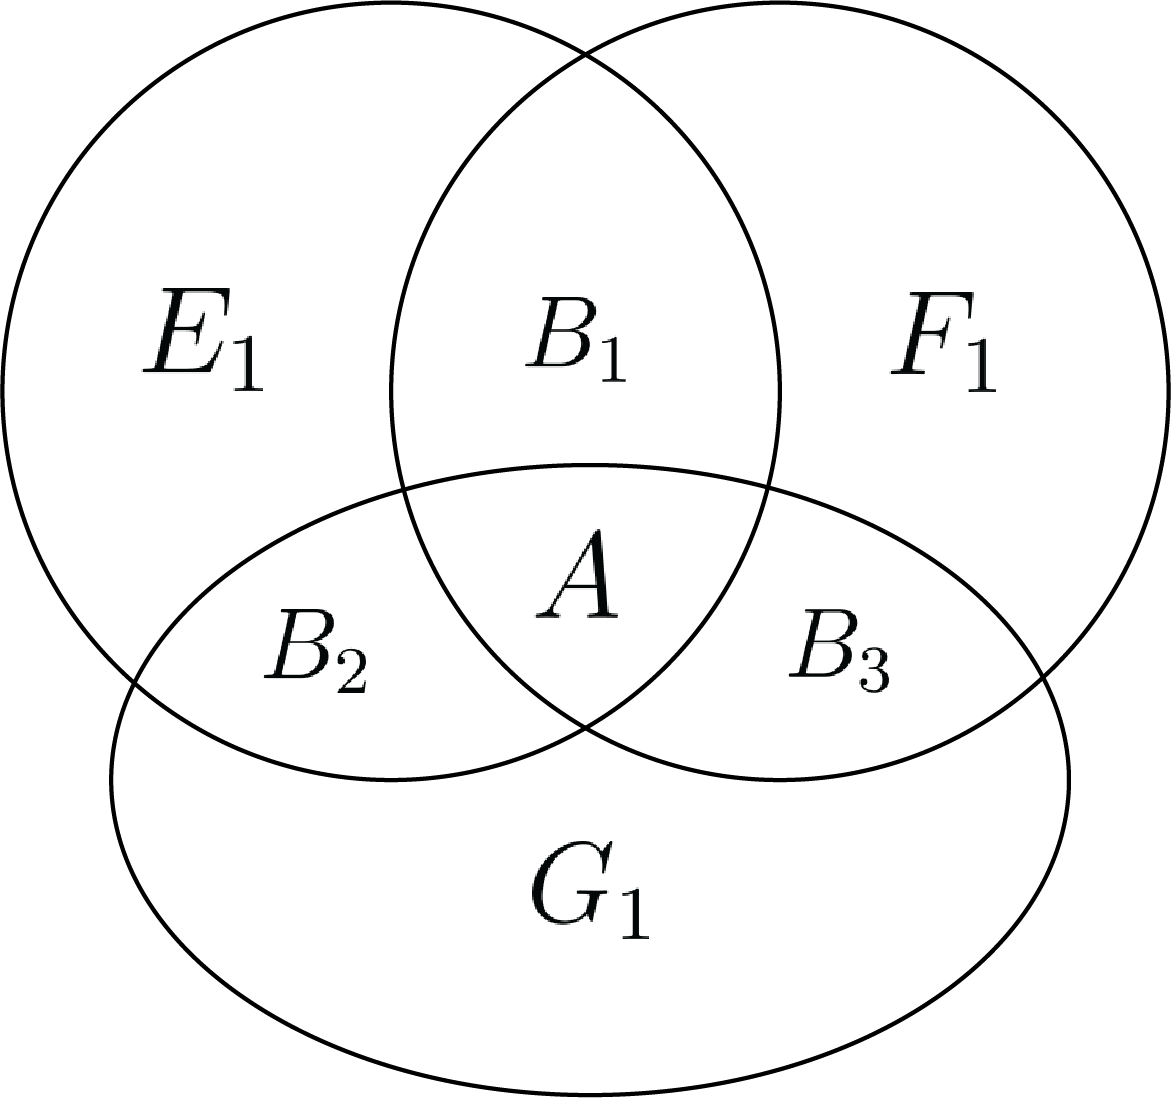
\includegraphics[scale=0.6]{figure/Venn_1.png}
        %\caption{Caption}
    \end{figure}
    
    令
    \begin{align*}
        &A = E \cap F \cap G, \\
        &B_1 = (E \cap F) \setminus A, \quad B_2 = (E \cap G) \setminus A, \quad B_3 = (F \cap G) \setminus A, \\
        &E_1 = E \setminus (B_1 \cup B_2 \cup A), \quad
         F_1 = F \setminus (B_1 \cup B_3 \cup A), \quad
         G_1 = G \setminus (B_2 \cup B_3 \cup A).
    \end{align*}
    则由条件知
    \begin{align*}
        &\mu(E_1 \cup B_2) + \mu(F_1 \cup B_3) = \mu(E_1)+\mu(B_2)+\mu(F_1)+\mu(B_3)=0, \\
        &\mu(F_1 \cup B_1) + \mu(G_1 \cup B_2) = \mu(F_1)+\mu(B_1)+\mu(G_1)+\mu(B_2)=0,
    \end{align*}
    则
    $$\mu(E \Delta G)
    = \mu(E_1 \cup B_1)+\mu(G_1 \cup B_3) 
    = \mu(E_1) + \mu(B_1) + \mu(G_1) + \mu(B_3) = 0. $$
    \end{enumerate}
    \qed 
\end{proof}
\begin{example}[~容斥原理(inclusion–exclusion principle)]
    现在我们介绍概率论中常用的\textbf{容斥原理}. 为此, 我们先引入概率测度$\P$. 设$(X, \calF, \P)$为一测度空间, 如果测度$\P$满足$\P(X) = 1$, 则称$(X,\calF,\P)$为一个\textbf{概率空间}(probability space), $\P$为其上的一个\textbf{概率测度}(probability measure), 简称概率. 令练习 \ref{inclu-exclu-basic-case} 中的$\mu$为概率测度$\P$可得两个集合的容斥原理
    $$\P(E \cup F) = \P(E)+\P(F) - \P(E \cap F). $$
    再次利用上一个例子中的Venn图, 我们有
    \begin{align*}
        E \cup F \cup G
        &= E \cup F_1 \cup B_3 \cup G_1 \\
        &= E \cup (F \setminus (A \cup B_1)) \cup (G \setminus (B_2 \cup B_3 \cup A)) \\
        &= E \cup (F \setminus (E \cap F)) \cup (G \setminus (B_2 \cup B_3 \cup A)), 
    \end{align*}
    则
    \begin{align*}
        \P(E \cup F \cup G)
        &= \P(E) + \P(F) - \P(E \cap F) + \P(G) - \P(B_2 \cup B_3 \cup A) \\
        &= \P(E)+\P(F)+\P(G) - \P(E \cap F) - [\P( (B_2 \cup A) \cup (B_3 \cup A) )] \\
        &= \P(E)+\P(F)+\P(G) - \P(E \cap F) - [\P( (B_2 \cup A) + \P(B_3 \cup A) - \P(A)] \\
        &= \P(E)+\P(F)+\P(G) - \P(E \cap F) - \P(E \cap G) - \P(F \cap G) + \P(E \cap F \cap G).
    \end{align*}
    但是对$n$个集合的情形, 我们就不能画Venn图了, 需要用数学归纳法. 一般地, 设$A_1, \cdots, A_n \in \calF$, 则
    \begin{equation}
    \P\br{\bCup{i=1}{n}A_i}
    = \Sum{i=1}{n}\P(A_i) - \sum_{i<j}\P(A_i \cap A_j) 
    + \sum_{i<j<k}\P(A_i \cap A_j \cap A_k) + \cdots + 
    (-1)^{n-1}\P\br{\bCap{i=1}{n}A_i}.
    \end{equation}
\end{example}
\begin{proof}
    假设容斥原理对$n$成立, 我们只需证明它对$n+1$也成立. 
    因为$\bCup{i=1}{n+1}A_i = \bCup{i=1}{n}A_i \cup A_{n+1}$, 所以我们可以套用$n=2$的容斥原理, 得
    $$\P\br{\bCup{i=1}{n}A_i \cup A_{n+1}}
    = \P\br{\bCup{i=1}{n}A_i} + \P(A_{n+1}) - \P\br{\bCup{i=1}{n}A_i \cap A_{n+1}}. $$
    这样右边最多就只有$n$个集合的并, 所以由归纳假设得
    \begin{align*}
    \P\br{\bCup{i=1}{n}A_i \cap A_{n+1}}
    &= \R\br{\bCup{i=1}{n} (A_i \cap A_{n+1})} \\
    &= \Sum{i=1}{n}\P(A_i \cap A_{n+1}) - \sum_{i<j \leq n}\P(A_i \cap A_j \cap A_{n+1}) 
    + \cdots + 
    (-1)^{n-1}\P\br{A_1 \cap \cdots \cap A_n \cap A_{n+1}},
    \end{align*}
    还有
    \begin{align*}
    \P\br{\bCup{i=1}{n}A_i}
    = \Sum{i=1}{n}\P(A_i) - \sum_{i<j \leq n}\P(A_i \cap A_j) 
    + \cdots + (-1)^{n-1}\P\br{A_1 \cap \cdots \cap A_n}.
    \end{align*}
    将上面两式相加, 得
    \begin{align*}
    \P\br{\bCup{i=1}{n}A_i \cup A_{n+1}}
    &= \Sum{i=1}{n+1}\P(A_i) - \sum_{i<j\leq n+1}\P(A_i \cap A_j)
    + \cdots \\
    &\quad + (-1)^{n-1}[\P(A_1 \cap \cdots \cap A_{n-1} \cap A_n) + 
                        \P(A_1 \cap \cdots \cap A_{n-1} \cap A_{n+1})] \\
    &\quad + (-1)^n \P(A_1 \cap \cdots \cap A_{n+1}),
    \end{align*}
    故容斥原理对$n+1$也成立, 所以对所有$n \in \N^+$都成立. \qed 
\end{proof}

%在利用Carath\'eodory条件证明勒贝格可测集对交, 并, 补的封闭性时,  也用到了这一思想. 
\subsection{Carath\'eodory条件中试验集的选取}
设$A \subset \R$, 若对任意集合$E \subset \R$, 有
\begin{equation}
    m^*(E) = m^*(E \cap A) + m^*(E \cap A^c), 
\end{equation}
则称$A$为勒贝格可测集, 而$E$一般可叫作\textbf{试验集}. 许多关于集合可测性结论的证明, 都依赖于试验集的巧取. 
\begin{exercise}[~(复习)]
    设$m^*$是$\R$上的勒贝格外测度, $A,B$为勒贝格可测集, 证明$A \cup B$也是勒贝格可测集. 
\end{exercise}
\begin{proof}
    设$E \subset \R$, 则
    \begin{align*}
    m^*(E) &= m^*(E \cap A) + m^*(E \cap A^c),
    \end{align*}
    因为$B$是可测集, 所以$B$满足Carath\'eodory条件, 分别取两个特殊的\textbf{试验集}$E \cap A$和$E \cap A^c$, 有
    \begin{align*}
    &m^*(E \cap A) = m^*((E \cap A) \cap B) + m^*((E \cap A) \cap B^c) \\
    &m^*(E \cap A^c) = m^*((E \cap A^c) \cap B) + m^*((E \cap A^c) \cap B^c).
    \end{align*}
    于是, 我们有
    $$ m^*(E) =  m^*(E \cap A \cap B) + m^*(E \cap A \cap B^c) + 
    m^*(E \cap A^c \cap B) + m^*(E \cap A^c \cap B^c), $$
    不难发现
    $$(E \cap A \cap B) \cup (E \cap A \cap B^c) \cup (E \cap A^c \cap B) \supset E \cap (A \cup B), $$
    所以由外测度的单调性得
    $$ m^*(E) \geq m^*(E \cap (A \cup B)) + m^*(E \cap (A \cup B)^c). $$
    \qed 
\end{proof}


\begin{example}\label{Caratheodory_thm}
    对集合$X$上的抽象外测度$\mu^*$, 我们也有Carath\'eodory条件, 还会给满足这个条件的集合起个新名字. 若集合$A \subset X$满足
    $$\mu^*(E) = \mu^*(E \cap A) + \mu^*(E \cap A^c) \text{ 对所有 }E \subset X\text{ 都成立},$$
    则称$A$是$\mu^*$-\textbf{可测}的. 设$\calM$是由所有$\mu^*$-可测集构成的集族, 则$\calM$是一个$\sigma$-代数.
\end{example}
\begin{proof}
    若$A,B \in \calM$, 则将上一条练习中的$m^*$改成$\mu^*$得$A \cup B \in \calM$. 现在我们证明对任意两两不交的可测集列$\{A_j\}_{j=1}^{\infty}$, 有$\bCup{j=1}{\infty}A_j \in \calM$. 也就是说, 我们要证明
    $$\mu^*(E) \geq \mu^*\br{E \cap \bCup{j=1}{\infty}A_j} + \mu^*\br{E \cap \bCap{j=1}{\infty}A_j^c}. $$
    我们先从有限多个的情形入手. 设$B_n = \bCup{j=1}{n}A_j, B = \bCup{j=1}{\infty}A_j$, 则对可测集$A_n$取\textbf{试验集}$E \cap B_n$, 得
    \begin{align*}
    \mu^*(E \cap B_n) &= \mu^*(E \cap B_n \cap A_n) + \mu^*(E \cap B_n \cap A_n^c) \\
    &= \mu^*(E \cap A_n) + \mu^*(E \cap B_{n-1}).
    \end{align*}
    同样, $\mu^*(E \cap B_{n-1}) = \mu^*(E \cap A_{n-1}) + \mu^*(E \cap B_{n-2})$. 故由数学归纳法得
    $$\mu^*(E \cap B_n) = \Sum{j=1}{n} \mu^*(E \cap A_j). $$
    因为每个$A_n$都是可测集, 所以$B_n$也是可测集, 选取\textbf{试验集}$E$得
    \begin{align*}
    \mu^*(E) &= \mu^*(E \cap B_n) + \mu^*(E \cap B_n^c) \\
    &\geq \Sum{j=1}{n}\mu^*(E \cap A_j) + \mu^*(E \cap B_c).
    \end{align*}
    令$n \to \infty$, 得
    \begin{align*}
    \mu^*(E) 
    &\geq \Sum{j=1}{\infty}\mu^*(E \cap A_j) + \mu^*(E \cap B^c) \\
    &\geq \mu^*\br{\bCup{j=1}{\infty}(E \cap A_j)} + \mu^*(E \cap B^c) \\
    &= \mu^*(E \cap B) + \mu^*(E \cap B^c) \geq \mu^*(E). 
    \end{align*}
    这就证明了$B=\bCup{j=1}{\infty}A_j$满足Carath\'eodory条件, 所以$B \in \calM$.  \qed 
\end{proof}
\begin{exercise}
    我们知道外测度$\mu^*$的定义域是$X$的所有子集构成的集族$\calP(X)$, 而测度则需要由外测度限制而来. 符号书接上例, 证明:
    $\mu^*$限制在$\sigma$-代数$\calM$上是一个测度. 
\end{exercise}
\begin{proof}
    因为$E$可以任取, 所以令$E=B$, 得
    $$\mu^*\br{\bCup{j=1}{\infty}A_j} = \Sum{j=1}{\infty}\mu^*(A_j), $$
    故$\mu^*$在$\calM$上满足可数可加性, 所以$\mu^*|_\calM$是一个测度. \qed 
\end{proof}
\begin{exercise}
    设$\mu^*$是集合$X$上的一个外测度, $\{A_j\}_{j=1}^\infty$为一列互不相交的$\mu^*$-可测集. 证明对任意$E \subset X$, 有
    $$\mu^*\br{E \cap \br{\bCup{j=1}{\infty}A_j} } = \Sum{j=1}{\infty}\mu^*(E \cap A_j). $$
\end{exercise}
%\begin{proof}
    %由外测度的可数次可加性得
    %$$\mu^*\br{E \cap \br{\bCup{j=1}{\infty}A_j} } \leq \Sum{j=1}{\infty}\mu^*(E \cap A_j),$$
    %所以另一个方向会比较难.
    %设$B_n = \bCup{j=1}{n}A_j, B = \bCup{j=1}{\infty}A_j$,则
    %\begin{align*}
    %\mu^*(E \cap B_n) &= \mu^*(E \cap B_n \cap A_n) + \mu^*(E \cap B_n \cap A_n^c) \\
    %&= \mu^*(E \cap A_n) + \mu^*(E \cap B_{n-1}).
    %\end{align*}
    %类似地, $\mu^*(E \cap B_{n-1}) = \mu^*(E \cap A_{n-1}) + \mu^*(E \cap B_{n-2})$. 故由数学归纳法得
    %$$\mu^*(E \cap B_n) = \Sum{j=1}{n} \mu^*(E \cap A_j). $$
    %因为$\mu^*$-可测集构成的集族是一个$\sigma$-代数, 所以$B_n, B$都是$\mu^*$-可测的, 于是根据Carath\'eodory条件, 得
    %由外测度的单调性, 可得
    %$$\mu^*(E \cap B) \geq \mu^*(E \cap B_n) = \Sum{j=1}{n} \mu^*(E \cap A_j) $$
    %令$n \to \infty$, 得
    %$$\mu^*(E \cap B) \geq \Sum{j=1}{\infty} \mu^*(E \cap A_j), $$
    %这就是另一个方向的不等式. \qed 
%\end{proof}

% ============== input: Cantor set and Borel measure
\section{康托集}
康托集一开始由康托提出, 目的是打破人们对于集合性质的一些常规认知, 
后来康托集也成为几何测度论中的一个重要研究对象. 该集合的勒贝格测度为$0$, 所以Lebesgue测度并不能很好地展现出Cantor集的特点. 今后我们会学习Hausdorff测度, 并且证明Cantor集的Hausdorff维数为 $\log 2 / \log 3$.
\subsection{定义与性质}
康托集有两个等价定义, 我们在正课中均已见过:
\begin{enumerate}
%\everymath{\displaystyle}
    \item 从$[0,1]$出发, 第一次挖掉$[\frac{1}{3}, \frac{2}{3}]$, 
    剩下来的集合记作$C_1$,
    第二次在$C_1$上挖掉$[\frac{1}{9}, \frac{2}{9}] \cup [\frac{7}{9}, \frac{8}{9}]$, 剩下来的集合记作$C_2$, 这样无限进行下去得Cantor集$\calC = \bigintersect{k=1}{\infty}C_k$.
    \item $[0,1]$中的实数可以写成三进制形式: $x = \Sum{k=1}{\infty}a_k/3^k$, 其中每个$a_k \in \{0,1,2\}$. Cantor集也可定义为
    $$\calC = \curlBrace{x=\Sum{k=1}{\infty}\frac{a_k}{3^k}: a_k \in \{0,2\}}.$$
\end{enumerate}
\begin{remark}
    根据无穷级数得知识可知
    $$\frac{1}{3} = \frac{1}{3^2}+\frac{1}{3^3}+\frac{1}{3^4}+\cdots,$$
    而$1/3$显然等于它自己, 于是同一个数就会有两种不同的三进制表示, 所以我们约定这种情况总是取无穷级数的表示.
\end{remark}
我们再复习一下Cantor集的性质:
\begin{property}
    \begin{enumerate}
    \item $\calC$是紧集;
    \item $m(\calC)=0$;
    \item $\calC$具有连续基数;
    \item $\calC$无处稠密, 即$\cl{\calC}^\circ=\varnothing$;
    \item $\calC$完全不连通(totally disconnected), 即任取$x,y \in \calC$, 总能找到$z \in (x,y): z \notin \calC$. 
    \item $\calC$无孤立点, 即$\calC$是一个完全(perfect)集.
    \end{enumerate}
\end{property}
\subsection{康托-勒贝格函数}
我们可以把$\calC$中的三进制小数映射到二进制小数. 
Cantor-Lebesgue函数的定义为$F:[0,1] \to [0,1]$,
$$F\Brace{\Sum{k=1}{\infty}\frac{a_k}{3^k}} = \Sum{k=1}{\infty}\frac{b_k}{2^k}, \quad 
\text{其中~}b_k = \frac{a_k}{2}, a_k \in \{0,1,2\}.$$

\begin{exercise}
    证明$F$是满射, 即对每个$y \in [0,1]$都存在$x \in \calC$使$F(x)=y$.
\end{exercise}
从该练习可以得出$\calC$具有连续基数. 

\begin{exercise} % Stein ex 1-21
    证明存在一个连续函数将一个勒贝格可测集映射至一个不可测集. (提示: 考虑$[0,1]$的一个不可测子集, 以及它在康托-勒贝格函数下的原像)
\end{exercise}


\subsection{广义康托集}
康托集的构造过程很容易推广: 改一改挖掉的区间数, 改一改挖去的区间长度, 就能得到许多类康托集(Cantor-like sets)(或称康托型集, Cantor-type sets).
同样, 将康托集的一些性质归纳出来进行排列组合, 比如``完全不连通的紧集"等等. 我们也可以将这些集合归于类康托集. 为和正课讲义保持一致, 我们将上面这两种集合统称为``广义康托集". 接下来我们看看广义康托集的应用. 

\begin{example} % Stein ex 1-20
    举例: $A, B \subset \R$为闭集且$m(A)=m(B)=0$, 但$m(A+B)>0$.
\end{example}
\begin{proof}
    令$A = \calC, B = \calC / 2$. 
    \qed
\end{proof}


\begin{example}
    构造一个博雷尔集$A \subset [0,1]$满足
    $$ 0<m(A \cap I)<m(I) \quad \text{对所有区间}~I \subset [0,1]~\text{都成立}. $$
\end{example}






\begin{example}
    构造一个$\R$中的博雷尔集$A$满足
    $$ 0<m(A \cap I)<m(I) \quad \text{对所有区间}~I~\text{都成立}. $$
\end{example}
\begin{solution}
    % 先证明对所有有理区间成立
    ``构造"和``对所有"明示了这道题的难度非同寻常, 我们必须简化``对所有区间"这个条件. 回想有理数集在实数集中的稠密性, 我们可以尝试用有理区间代替所有区间. 如果我们能构造出$A$使结论对所有有理区间都成立, 那么该结论也应该对所有区间都成立. 现在我们来论证这个陈述:

    设$\Q = \{r_1, r_2, \cdots\}$, 假设我们已经构造出了博雷尔集$A$满足
    $$0 < m(A \cap (r_i,r_j)) < r_j - r_i \quad \text{对所有}~r_i<r_j~\text{都成立}.$$
    现任取一区间$I=(a,b)$(只需考虑开区间即可, 为什么?), 则可以找到有理数$a<r_i<r_j<b$. 接下来,
    \begin{align*}
    m(A \cap I)
    &= m(A \cap (a,r_i)) + m(A \cap (r_i,r_j)) + m(A \cap (r_j,b)) \\
    &< (r_i-a) + (r_j - r_i) + (b-r_j) \\
    &= b-a,
    \end{align*}
    且$m(A \cap I) \geq m(A \cap (r_i-r_j)) > 0$, 故结论对所有区间$I$都成立. 

    至此, 我们已将题目简化为了``构造一个$\R$中的博雷尔集$A$满足$0<m(A \cap I)<m(I)$对所有有理区间$I$都成立."
    
\end{solution}

% https://www.jstor.org/stable/pdf/2975692.pdf?refreqid=excelsior%3A200cfff310a747c5a4b7f4620fd7f019&ab_segments=&origin=&acceptTC=1
\section{$\R$上的博雷尔测度与分布函数}
\begin{exercise}
    设$F$单调递增且右连续, 令$\mu_F$为分布函数$F$对应的测度. 证明
    \begin{enumerate}
    \item $\mu_F(\{a\})=F(a)-F(a^-)$,
    \item $\mu_F([a,b])=F(b)-F(a^-)$,
    \item $\mu_F([a,b))=F(b^-) - F(a^-)$,
    \item $\mu_F((a,b))=F(b^-)-F(a)$. 
    \end{enumerate}
\end{exercise}
\begin{proof}
    $\mu_F$与$F$以左开右闭区间为纽带: $\mu_F((a,b]) = F(b)-F(a)$, 所以我们要想法设法将题中的集合转化到左开右闭区间上. 
    \begin{enumerate}
    \item 因为$\{a\} = \bCap{n=1}{\infty}(a-1/n, a]$, 所以由测度的单调收敛定理得
    $$\mu_F\br{\bCap{n=1}{\infty}(a-1/n, a]} = \lim_{n \to \infty}\mu_F((a-1/n,a])
    = \lim_{n \to \infty}[F(a)-F(a-1/n)] = F(a) - F(a^-). $$
    \item $[a,b] = \{a\} \cup (a,b]$;
    \item $[a,b) = [a,b] \setminus \{b\}$;
    \item $(a,b) = (a,b] \setminus \{b\}$.
    \end{enumerate} \qed 
\end{proof}
由该练习立刻可得:
\begin{exercise}
    $F$连续当且仅当$\mu_F(\{a\}) = 0$对所有单点集$\{a\} \subset \R$都成立. 
\end{exercise}

\begin{example}\label{Cantor_measure}\footnote{部分参考UW-Madison博士资格考试题}
    设$\sigma$是$[0,1]$上的博雷尔测度, 且满足以下条件:
    \begin{enumerate}
    \item $\sigma([0,1]) = 1$;
    \item $\sigma([1/3, 2/3]) = 0$;
    \item $\sigma([a,b]) = \sigma([1-b,1-a])~\forall 0 \leq a < b \leq 1$;
    \item $\sigma([3a, 3b]) = 2\sigma([a,b])$对所有满足$0 \leq 3a < 3b \leq 1$的$a,b$都成立. 
    \end{enumerate}
    称这个$\sigma$为$[0,1]$上的$\frac{1}{3}$-康托测度. 
    \begin{enumerate}
        \item 求$\sigma([0, 1/8])$.
        \item 证明康托-勒贝格函数$F$对应的博雷尔测度$\mu_F$满足$\sigma$的4条性质(将题中4条性质中的$\sigma$替换成$\mu_F$)
        \item\footnote{出次阅读时可跳过该问} 证明$\sigma$对应的分布函数$F$就是康托-勒贝格函数
    \end{enumerate}
\end{example}
%\begin{remark}
    %本题第二问较难, 如果你对抽象测度的构造过程不熟悉, 可以将第二问改成``", 这样就可以避开唯一性的讨论.  
%\end{remark}
\begin{proof}
    \textbf{(1)}
    由$\sigma([0, 1/3]) = \sigma([2/3, 1])$以及
    $$1=\sigma([0,1]) = \sigma([0, 1/3]) + \sigma([2/3, 1]) + \sigma([1/3, 2/3])$$
    得$$\sigma([0, 1/3]) = \sigma([2/3, 1]) = \frac{1}{2}. $$
    由第4条性质得
    $$ \sigma\br{\left[ \frac{1}{9},\frac{2}{9} \right]} = 
       \frac{1}{2}\sigma\br{\left[ 3 \times \frac{1}{9},3 \times \frac{2}{9} \right]} = \frac{1}{2}\sigma\br{\left[ \frac{1}{3},\frac{2}{3} \right]} = 0, $$
    且$$ \sigma\br{\left[ 0,\frac{1}{9} \right]} = \frac{1}{2} \sigma\br{\left[ 0, 3 \times \frac{1}{9} \right]} = \frac{1}{2} \times \frac{1}{2} = \frac{1}{4}. $$
    所以
    $$\sigma\br{\left[ 0,\frac{1}{8} \right]} = \sigma\br{\left[ 0,\frac{1}{9} \right]} + \sigma\br{\left[ \frac{1}{9},\frac{1}{8} \right]} = \frac{1}{4} + 0 = \frac{1}{4}. $$
    \textbf{(2)} 接下来, 我们检验: 
    \begin{itemize}
    \item $F(1) - F(0) = 1$;
    \item $F(2/3) - F(1/3) = 0$;
    \item $F(b) - F(a) = F(1-a) - F(1-b)$;
    \item $F(3b) - F(3a) = 2(F(b) - F(a))$.
    \end{itemize}
    前两条不言自明. 先将$F$限制在康托集$\calC$上. 
    {\everymath{\displaystyle}
    记$a = \Sum{k=1}{\infty}\frac{a_k}{3^k}, b = \Sum{k=1}{\infty}\frac{b_k}{3^k}$, 
    其中$a_k, b_k \in \{0, 2\}$, 则
    $$ 1-a = \Sum{k=1}{\infty}\frac{2}{3^k} - \Sum{k=1}{\infty}\frac{a_k}{3^k}
    = \Sum{k=1}{\infty}\frac{2-a_k}{3^k}, \quad 
    1-b = \Sum{k=1}{\infty}\frac{2}{3^k} - \Sum{k=1}{\infty}\frac{b_k}{3^k}
    = \Sum{k=1}{\infty}\frac{2-b_k}{3^k}.
    $$
    于是
    \begin{align*}
    &F(1-a) - F(1-b) = \Sum{k=1}{\infty}\frac{1-a_k/2}{3^k} - \Sum{k=1}{\infty}\frac{1-b_k/2}{3^k} = \Sum{k=1}{\infty}\frac{(a_k-b_k)/2}{3^k} \\
    &F(b)-F(a) = \Sum{k=1}{\infty}\frac{b_k/2}{3^k}-\Sum{k=1}{\infty}\frac{a_k/2}{3^k} = \Sum{k=1}{\infty}\frac{(a_k-b_k)/2}{3^k}.
    \end{align*}
    同理可证$F(3b) - F(3a) = 2(F(b) - F(a))$.
    若$a,b \in [0,1] \setminus \calC$, 则由先前的练习, 有
    $$F(1-a) =  \sup_{s \geq a, s \in \calC} F(1-s) = \inf_{s \leq a, s \in \calC} F(1-s).$$ 
    这样做是为了将$F(a)$和$F(1-a)$中上下确界的指标集统一起来. 
    接下来我们利用确界的定义证明两个方向的不等式. 
    
    设$\eps > 0$, 则由$F(a), F(b)$的上确界定义知存在$x_0, y_0 \in \calC, x_0 \leq a, y_0 \leq b$, 使得
    $$F(a) \geq F(x_0) > F(a)-\eps, \quad F(b) \geq F(y_0) > F(b)-\eps. $$
    这里的$x_0, y_0$只是一个基准. 更进一步, 由$F$的单调性得
    $$F(a) \geq F(x) > F(a)-\eps, \quad F(b) \geq F(y) > F(b)-\eps \quad \text{对所有 }x \in [x_0,a] \cap \calC, y \in [y_0, b] \cap \calC \text{ 都成立}. $$
    
    于是$$ -F(a) \leq -F(x) < \eps - F(a), $$
    从而
    $$F(1-x)-F(1-y) = F(y)-F(x) > F(b)-F(a)-\eps. $$
    移项, 得
    $$F(1-x) > F(b)-F(a) + F(1-y) - \eps, $$
    
    对$y$取下确界, 根据$F(1-b) = \inf_{y \leq b, y \in \calC}F(1-y)$得
    $$F(1-x) \geq F(b)-F(a) + F(1-b) - \eps, $$ 再对$x$取下确界, 得
    $$F(1-a) - F(1-b) \geq F(b)-F(a)-\eps. $$ 因为$\eps$是任意的, 所以
    $$F(1-a) - F(1-b) \geq F(b) - F(a). $$
    反过来, 对任意的$\eps > 0$, 存在$x_0, y_0 \in \calC, x_0 \leq a, y_0 \leq b$, 使得
    $$F(1-a) \geq F(1-x_0) > F(1-a) - \eps, \quad F(1-b) \geq F(1-y_0) > F(1-b) $$
    由于$F(1-t)$是关于$t$的单调递减函数, 则对所有$x \in [x_0,a] \cap \calC, y \in [y_0, b] \cap \calC$都有
    $$F(1-a) \geq F(1-x) > F(1-a)-\eps, \quad F(1-b) \geq F(1-y) > F(b)-\eps. $$
    类似地, 我们有
    $$F(1-a)-F(1-b) \leq F(b) - F(a). $$
    同理可证, 若$a,b \in [0,1] \setminus \calC$, 则$F(3b)-F(3a) = 2(F(b)-F(a))$.
    所以$F$对应的博雷尔测度$\mu_F$满足$\sigma$的4个条件.} \\
    \textbf{(3)}   
    记$F$为康托-勒贝格函数, 我们已知$F$是$[0,1]$上单调增的连续函数, 所以有一个唯一的博雷尔测度$\mu_F$与之对应.
    你可能会想: 满足题中4个条件的博雷尔测度$\sigma$是唯一的吗? 
    因为$[0,1]$上的博雷尔$\sigma$-代数可由$\calE_1 = \{[a,b]: 0 \leq a < b \leq 1 \}$生成, 所以$\sigma$完全由$\sigma([a,b])$决定(详见测度的构造过程),
    %而$\sigma$在区间上的值由完全由其在康托集构造第$k$步中$C_k$的连通分支上的值所决定. 例如:
    %\begin{itemize}
        %\item 计算$\sigma([0,1/2])$, 只需用到第一步的$\sigma([0,1/3])=1/2$;
        %\item 计算$\sigma([0,1/8])$只需用到$C_2$.
    %\end{itemize}
    回顾康托集的构造过程, 我们在第$k$步得到了$2^k$个长度为$3^{-k}$的区间的无交并, 记为$C_k$. 记这些单独的闭区间(即连通分支)为$C_{k,j}, 1 \leq j \leq 2^k$. 根据$\sigma$的后两条性质以及数学归纳法, 我们有
    \begin{align*}
        &\sigma(C_1^c) = \sigma((1/3, 2/3)) = 0, \\
        &\sigma(C_2^c) = \sigma((1/9, 2/9) \cup (1/3, 2/3) \cup (7/9,8/9)) = 0, \\
        &\cdots \\
        &\sigma(C_k^c) = 0, \\
        &\cdots
    \end{align*}
    于是, $\sigma\br{\bCup{k=1}{\infty}C_k^c} = \sigma\br{ (\bCap{k=1}{\infty}C_k)^c } = \sigma([0,1] \setminus \calC) = 0$, 且对每个固定的$k$, 有
    $$\sigma(C_{k,j}) = \frac{1}{2^k} \quad (1 \leq j \leq 2^k). $$
    这样, $\sigma$在集族$\calE_2 = \{C_{k,j}: k \in \N, 1 \leq j \leq 2^k \}$上是唯一确定的.
    接下来, 我们只需说明: 如果$\sigma$在$\calE_2$上唯一确定, 则$\sigma$在$\calE_1$上唯一确定.
    我们先证明单点集的$\sigma$-测度为$0$. 
    \begin{itemize}
        \item 如果$a \in \calC$, 则$a \in C_k~\forall k$, 所以
        $$\sigma(\{a\}) \leq \sigma(C_k) = \br{\frac{2}{3}}^k ~\forall k, $$
        令$k \to \infty$得$\sigma(\{a\}) = 0$.
        \item 如果$a \notin \calC$, 则$$\sigma(\{a\}) \leq \sigma([0,1] \setminus \calC) = 0. $$ 
    \end{itemize}
    
    
    对任意的闭区间$[a,b]$, 我们可以将其拆分成两部分:
    $[a,b] = ([a,b] \cap \calC) \sqcup ([a,b] \cap \calC^c)$, 故
    \begin{align*}
        \sigma([a,b])
        &= \sigma([a,b] \cap \calC) + \sigma([a,b] \cap \calC^c) \\
        &= \sigma([a,b] \cap \calC) \\
        &= \sigma\br{\bCap{k=1}{\infty}[a,b] \cap C_k } \\
        &= \lim_{k \to \infty} \sigma([a,b] \cap C_k)
    \end{align*}
    现在, 我们来研究如何计算$\sigma([a,b] \cap C_k)$. 
    通过平移, $\sigma([a,b]) = \sigma([0, b-a])$, 
    所以我们不妨研究闭区间$[0,a], a > 0$.
    现在, 对$a$进行讨论:
    \begin{enumerate}
        \item 若$a \in (1/3, 2/3)$, 则$[0,a] \supset C_{1,1} = [0, 1/3]$, 所以$\sigma([0,a])=\sigma(C_{1,1}) = 1/2$. 
        \item 若$a \in [0, 1/3]$, 则$a \in [0, 1/9] \cup (1/9, 2/9) \cup [2/9, 1/3]$.
        \item 若$a \in [2/3, 1]$, 则只需考虑$[0, a] \cap [2/3, 1]$, 这跟$a \in [0, 1/3]$的情形没有区别. 所以接下来我们都考虑$a \in [0, 2/3^n]$的情形. 
        \item 由于$a>0$, 所以必定存在$k \in \N$, 使得$a \in (1/3^k, 2/3^k)$, 故$[0,a] \supset [0, 1/3^k] = C_{k, 1}$, 则$\sigma([0,a]) = \sigma(C_{k,1})$. 
        
    \end{enumerate}
    所以$\sigma$在闭区间上的值由$\sigma$在$\calE_2$上的值唯一确定. 再详细一点: 若$\mu$是另一个满足题中4个条件的博雷尔测度, 则由完全类似的过程可得$\mu([0,a]) = \mu(C_{k,j})$, 而那4条性质又告诉我们, $\mu(C_{k,j}) = 3^{-k}$, 所以
    $$\mu(C_{k,j}) = \sigma(C_{k.j}), $$ 从而$$\mu([0,a]) = \sigma([0,a]), $$
    故$$\mu([a,b]) = \sigma([a,b]). $$
    
    %这样, $\sigma$对应的唯一的分布函数$F_\sigma$就是连续的, 且必满足
    %\begin{align*}
        %&\sigma([a,b])=F_\sigma(b) - F_\sigma(a), \\
        %&F_\sigma(b) - F_\sigma(a) = F_\sigma(1-a) - F_\sigma(1-b) \\
        %&F_\sigma(3b) - F_\sigma(3a) = 2(F_\sigma(b) - F_\sigma(a)).
    %\end{align*}
    %这4条性质足以让我们对每个$k \in \N$, 计算出$\sigma$在$C_k$的连通分支上的值. 因而我们只需要证明
    现在, 我们证明康托-勒贝格函数$F$对应的博雷尔测度$\mu_F$满足$\sigma$的4个条件. 由于$F$连续, 所以
    $$F(b)-F(a) = \mu_F([a,b]). $$ 
\end{proof}

\begin{exercise}
    书接上例, 在不验证康托-勒贝格函数$F$对应的博雷尔测度满足那4条性质的情况下, 证明$\sigma$对应的分布函数$F_\sigma$是康托-勒贝格函数.
\end{exercise}
\begin{proof}
    由博雷尔测度的分布函数的定义知, $F_\sigma(a) = \sigma((0, a])$.
    由上例的证明过程知$\sigma$在单点集处的测度为$0$, 所以$F_\sigma(a) = \sigma([0,a])$.
    一般地, 我们有$F_\sigma(b)-F_\sigma(a) = \sigma([a,b])$. 接下来分$a \in \calC$和$a \notin \calC$两种情况讨论. 若$a \in \calC$, 则利用三进制小数证明$F_\sigma(a) = F(a)$. 细节留作练习. \qed
\end{proof}


\section{可测集与测度的性质}
\subsection{点集间的距离}
我们先补充一些预备知识. 如果你已对此节内容比较熟悉, 请速速跳过.
首先定义点与集合间的距离. 设$E \subset \R^n, x \in \R^n$, 定义$x$与$E$的\textbf{距离}为
$$d(x,E) = \inf_{y \in E} |x-y|, $$
其中$|x-y| = \sqrt{(x_1-y_1)^2 + \cdots + (x_n-y_n)^2}$.
\begin{example}
    设$E \subset \R^n$, 则$d(x,E) = 0 \iff x \in \cl{E}$. 
\end{example}
\begin{proof}
    若$x \in \cl{E}$, 则存在$\{y_n\} \subset E$使得$\lim_{n \to \infty}y_n = x$, 所以$\inf_{n \in \N}|x-y_n| = 0$, 故$d(x,E) = 0$. 反过来, 若$\inf_{y \in E}|x-y| = 0$, 则存在$E$中的点列$\{y_n\}$满足$|y_n - x| \to 0$, 所以$x \in \cl{E}$. \qed 
\end{proof}
\begin{exercise}
    设$F \subset \R^n$为闭集, 则$d(x,F) = 0 \iff x \in F$.
\end{exercise}
\begin{exercise}
    证明: $d(x,E) = d(x, \cl{E})$. 
\end{exercise}
\begin{example}
    固定集合$E \subset \R^n$, 我们可以将$d(x,E)$看作$x$的函数, 即定义
    \begin{align*}
        f: \R^n &\to [0,\infty) \\
        f(x) &= d(x,E).
    \end{align*}
    证明: $f$是一个连续函数. 
\end{example}
\begin{proof}
    设$x_n \to x$, 我们证明$d(x_n,E) \to d(x,E)$. 设$y \in E$, 则$|x-y| \leq |x-x_n| + |x_n-y|$, 从而
    \begin{align*}
        &|x-y|-|x_n-y| \leq |x-x_n|, \\
        &|x_n-y| - |x-y| \geq -|x-x_n|.
    \end{align*}
    设$\eps>0$, 则存在$N \in \N$使得$|x_n - x|<\eps~\forall n > N$. 从而
    \begin{align*}
        &|x_n-y| \leq \eps + |x-y|, \\
        &|x_n-y| \geq |x-y|-\eps.
    \end{align*}
    两边对$y$取下确界得
    \begin{align*}
        &d(x_n,E)-d(x,y) \leq \eps, \\
        &d(x_n,E)-d(x,y) \geq -\eps.
    \end{align*}
    也就是说, 对任意$\eps>0$都存在$N\in\N$使得$n>N$时, $|d(x_n,E)-d(x,y)| \leq \eps$, 所以
    $$\limsup_{n\to \infty}|d(x_n,E)-d(x,y)|=0. $$
    由归结原则知$f(x)=d(x,E)$连续. \qed    
\end{proof}
今后我们会利用距离函数的连续性(开集的原像是开集)构造一些开集, 例如$U_n := \{x \in \R^n: d(x,E) < 1/n\}$.

现在看点集与点集间的距离. 我们的定义还是基于点与点的距离, 不过这次要让两个点都动起来. 设$E,F \subset \R^n$, 定义$E$与$F$的\textbf{距离}为
$$d(E,F) = \inf\{|x-y|: x \in E, y \in F\}.$$

对单独的一个集合$A$, 定义其\textbf{直径}(diameter)为$d(A) = \sup_{x,y \in A} |x-y|$. 由于不会引起歧义, 我们仍采用字母$d$. 
\subsection{测度的单调收敛定理}
设$E_1 \subset E_2 \subset \cdots $为一单调递增的集列, 记$E = \bigunion{n=1}{\infty}E_n$, 则
$$m(E)=\lim_{n \to \infty}m(E_n).$$
若使用集合列极限的记号, 上式可以写得更直观:
$$m(E)=m\left(\bigunion{n=1}{\infty}E_n\right)=m(\Lim{n}{\infty}E_n) = \Lim{n}{\infty}m(E_n).$$
设$F_1 \supset F_2 \supset \cdots $为一单调递减的集列且$m(F_1)<\infty$,
记$F = \bigintersect{n=1}{\infty}F_n$, 则
$$m(F)=\lim_{n \to \infty}m(F_n).$$
等式也可以写成:
$$m(F)=m\left(\bigintersect{n=1}{\infty}F_n\right)=m(\Lim{n}{\infty}F_n) = \Lim{n}{\infty}m(F_n).$$
\begin{exercise}
    在$\R$中试找出一列$\{F_n\}_{n=1}^\infty,$ 但$m(F_1)=\infty$, 
    使得$m\br{\bCap{n=1}{\infty}F_n} \neq \lim_{n \to \infty}m(F_n)$.
\end{exercise}
% 18.8


\subsection{勒贝格可测集的正则性质}
由于$\R^n$具备天然的拓扑结构(由欧几里得范数$\|x\|=\sqrt{x_1^2 + \cdots + x_n^2}$所引出), 我们可以用熟悉的集合(开集, 闭集, 紧集)逼近一般的勒贝格可测集. 
设$E$是$\R^n$中的一个可测集, 则对任意$\eps>0$:
\begin{enumerate}
    \item 存在开集$U \supset E$使$m(U \setminus E)\leq \eps$.
    \item 存在闭集$F \subset E$使$m(E \setminus F)\leq \eps$.
    \item 若$m(E)<\infty$, 则存在紧集$K\subset E$使$m(E \setminus K) \leq \eps$. 
    %\item 若$m(E)<\infty$, 则存在有限多个方体$\{Q_j\}_{j=1}^N$使
    %$$m\left(E \Delta \bigunion{j=1}{N}Q_j\right) \leq \eps.$$
\end{enumerate}
如果将$\eps$离散化, 即对每个$n \in \N$存在开集$U_n \supset E$使$m(U_n \setminus E) \leq 1/n$, 然后取极限(相关证明参见正课), 我们可以将勒贝格可测集表达成一个博雷尔集并上或减去一个零测集的形式:
\begin{enumerate}
    \item $E \subset \R^n$可测当且仅当$E=G \setminus N$, 其中$G$是一个$G_\delta$集, $N$是一个零测集;
    \item $E \subset \R^n$可测当且仅当$E=F \cup M$, 其中$F$是一个$F_\sigma$集, $M$是一个零测集. 
\end{enumerate}
后续我们会学习定义在可测集上的函数以及在可测集上做积分, 研究这些函数和积分的性质时我们往往会遵循从简单到复杂的顺序: 
方体$\rightarrow$开集$\rightarrow$可数个开集的交($G_\delta$)$\rightarrow$可测集. 现在请大致在脑海中留下这个印象: “勒贝格可测集可以表达成更简单的形式”. 不必强行记忆这6条性质(但是要确保自己动手证明过一遍), 它们会在后续内容中反复出现, 等你学完实分析之后就会发现自己根本忘不掉! 
\begin{exercise} % Stein 1-25
    可测性的另一种等价定义: 若对任意$\eps>0$都存在闭集$F \subset E$, 使得$m^*(E \setminus F) < \eps$, 则$E$可测. 证明该定义与``开集逼近"条件等价.     
\end{exercise}
\begin{proof}
    提示: 注意到$U \setminus E = U \cap E^c = E^c \cap (U^c)^c = E^c \setminus U^c$.
\end{proof}
\begin{exercise}
    给定集合$E$, 设
    $$U_n = \{x: d(x,E)<1/n\}.$$ 证明
    \begin{enumerate}
    \item 如果$E$是紧集, 则$m(E)=\lim_{n\to \infty}m(U_n)$.
    \item 如果$E$闭且无界, 则结论不一定成立.
    \item 如果$E$开且有界, 则结论不一定成立.
    \end{enumerate}
\end{exercise}
\begin{proof}
    \begin{enumerate}
    \item 显然$U_1 \supset U_2 \supset \cdots$为一递减集列, 且因为$E$是紧集, 所以$m(U_1) < \infty$. 
    现在只需证$E = \bCap{n=1}{\infty}\{x:d(x,E) < 1/n\}$. 设$x \in E$, 则$d(x,E)=0$. 设$x \in  \bCap{n=1}{\infty}\{x:d(x,E) < 1/n\}$, 则$d(x,E) < 1/n~\forall n \in \N$, 故$d(x,E) = 0$, 所以$x \in \cl{E} = E$. 
    \item 令$E = \Z$, 则对每个$n \in \N$, 都有
    $$m(U_n) \geq \frac{2}{n} \cdot n = 2, $$
    而$m(E) = 0$. 
    \item 注意到$\cl{E}$是紧集, 所以(1)对$\cl{E}$成立, 于是问题肯定出在$\partial E$上, 故联想到稠密性. 记$D=(0,1) \cap \Q = \{r_1, r_2, \cdots\}$, 令$\eps < 1$, 对每个$r_n$, 令$E_n = (r_n - 2^{-n}\eps, r_n + 2^{-n}\eps)$, 则$E := (\bCup{n=1}{\infty}E_n) \cap (0,1)$是开集, 
    且$$ 1 = m([0,1]) = m(\cl{E}) = \lim_{n \to \infty}m(U_n), $$
    但是$m(E) < \eps$. \qed 
    \end{enumerate}
\end{proof}

现在我们略微研究一下$G_\d$和$F_\sigma$集.
\begin{exercise}\footnote{本练习第2条需要用到Baire纲定理, 可跳过.}
    \begin{enumerate}
    \item 证明闭集都是$G_\d$集, 开集都是$F_\sigma$集.
    \item 想出一个不是$G_\d$集的$F_\sigma$集.
    %\item 想出一个既不是$G_\d$也不是$F_\sigma$的博雷尔集. 
    \end{enumerate}
\end{exercise}
\begin{proof}
    \begin{enumerate}
    \item 设$F$是一个闭集, 令$U_n = \{x: d(x,F) < 1/n\}$, 则$U_n$是开集, 且$F = \bCap{n=1}{\infty}U_n$. 任一开集都可以写成可数个闭方体的并, 所以为$F_\sigma$集. 
    \item 我们证明有理数集$\Q$满足要求. 首先, $\Q = \bCup{n=1}{\infty}\{r_n\}$显然是个$F_\sigma$集. 
    \end{enumerate}
\end{proof}
\begin{exercise} % Stein 1.27
    设$E_1,E_2$为$\R$中的紧集, $E_1 \subset E_2$. 令$a = m(E_1), b = m(E_2)$. 
    证明: 对任意$c \in (a,b)$, 都存在紧集$E$满足$E_1 \subset E \subset E_2$且$m(E)=c$. 
    (提示: 如果$E$为$[0,1]$的可测子集, 考虑$t$的函数$m(E \cap [0,t])$)
\end{exercise}

% 18.13

    %\section{康托集}
康托集一开始由康托提出, 目的是打破人们对于集合性质的一些常规认知, 
后来康托集也成为几何测度论中的一个重要研究对象. 该集合的勒贝格测度为$0$, 所以Lebesgue测度并不能很好地展现出Cantor集的特点. 今后我们会学习Hausdorff测度, 并且证明Cantor集的Hausdorff维数为 $\log 2 / \log 3$.
\subsection{定义与性质}
康托集有两个等价定义, 我们在正课中均已见过:
\begin{enumerate}
%\everymath{\displaystyle}
    \item 从$[0,1]$出发, 第一次挖掉$[\frac{1}{3}, \frac{2}{3}]$, 
    剩下来的集合记作$C_1$,
    第二次在$C_1$上挖掉$[\frac{1}{9}, \frac{2}{9}] \cup [\frac{7}{9}, \frac{8}{9}]$, 剩下来的集合记作$C_2$, 这样无限进行下去得Cantor集$\calC = \bigintersect{k=1}{\infty}C_k$.
    \item $[0,1]$中的实数可以写成三进制形式: $x = \Sum{k=1}{\infty}a_k/3^k$, 其中每个$a_k \in \{0,1,2\}$. Cantor集也可定义为
    $$\calC = \curlBrace{x=\Sum{k=1}{\infty}\frac{a_k}{3^k}: a_k \in \{0,2\}}.$$
\end{enumerate}
\begin{remark}
    根据无穷级数得知识可知
    $$\frac{1}{3} = \frac{1}{3^2}+\frac{1}{3^3}+\frac{1}{3^4}+\cdots,$$
    而$1/3$显然等于它自己, 于是同一个数就会有两种不同的三进制表示, 所以我们约定这种情况总是取无穷级数的表示.
\end{remark}
我们再复习一下Cantor集的性质:
\begin{property}
    \begin{enumerate}
    \item $\calC$是紧集;
    \item $m(\calC)=0$;
    \item $\calC$具有连续基数;
    \item $\calC$无处稠密, 即$\cl{\calC}^\circ=\varnothing$;
    \item $\calC$完全不连通(totally disconnected), 即任取$x,y \in \calC$, 总能找到$z \in (x,y): z \notin \calC$. 
    \item $\calC$无孤立点, 即$\calC$是一个完全(perfect)集.
    \end{enumerate}
\end{property}
\subsection{康托-勒贝格函数}
我们可以把$\calC$中的三进制小数映射到二进制小数. 
Cantor-Lebesgue函数的定义为$F:[0,1] \to [0,1]$,
$$F\Brace{\Sum{k=1}{\infty}\frac{a_k}{3^k}} = \Sum{k=1}{\infty}\frac{b_k}{2^k}, \quad 
\text{其中~}b_k = \frac{a_k}{2}, a_k \in \{0,1,2\}.$$

\begin{exercise}
    证明$F$是满射, 即对每个$y \in [0,1]$都存在$x \in \calC$使$F(x)=y$.
\end{exercise}
从该练习可以得出$\calC$具有连续基数. 

\begin{exercise} % Stein ex 1-21
    证明存在一个连续函数将一个勒贝格可测集映射至一个不可测集. (提示: 考虑$[0,1]$的一个不可测子集, 以及它在康托-勒贝格函数下的原像)
\end{exercise}


\subsection{广义康托集}
康托集的构造过程很容易推广: 改一改挖掉的区间数, 改一改挖去的区间长度, 就能得到许多类康托集(Cantor-like sets)(或称康托型集, Cantor-type sets).
同样, 将康托集的一些性质归纳出来进行排列组合, 比如``完全不连通的紧集"等等. 我们也可以将这些集合归于类康托集. 为和正课讲义保持一致, 我们将上面这两种集合统称为``广义康托集". 接下来我们看看广义康托集的应用. 

\begin{example} % Stein ex 1-20
    举例: $A, B \subset \R$为闭集且$m(A)=m(B)=0$, 但$m(A+B)>0$.
\end{example}
\begin{proof}
    令$A = \calC, B = \calC / 2$. 
    \qed
\end{proof}


\begin{example}
    构造一个博雷尔集$A \subset [0,1]$满足
    $$ 0<m(A \cap I)<m(I) \quad \text{对所有区间}~I \subset [0,1]~\text{都成立}. $$
\end{example}






\begin{example}
    构造一个$\R$中的博雷尔集$A$满足
    $$ 0<m(A \cap I)<m(I) \quad \text{对所有区间}~I~\text{都成立}. $$
\end{example}
\begin{solution}
    % 先证明对所有有理区间成立
    ``构造"和``对所有"明示了这道题的难度非同寻常, 我们必须简化``对所有区间"这个条件. 回想有理数集在实数集中的稠密性, 我们可以尝试用有理区间代替所有区间. 如果我们能构造出$A$使结论对所有有理区间都成立, 那么该结论也应该对所有区间都成立. 现在我们来论证这个陈述:

    设$\Q = \{r_1, r_2, \cdots\}$, 假设我们已经构造出了博雷尔集$A$满足
    $$0 < m(A \cap (r_i,r_j)) < r_j - r_i \quad \text{对所有}~r_i<r_j~\text{都成立}.$$
    现任取一区间$I=(a,b)$(只需考虑开区间即可, 为什么?), 则可以找到有理数$a<r_i<r_j<b$. 接下来,
    \begin{align*}
    m(A \cap I)
    &= m(A \cap (a,r_i)) + m(A \cap (r_i,r_j)) + m(A \cap (r_j,b)) \\
    &< (r_i-a) + (r_j - r_i) + (b-r_j) \\
    &= b-a,
    \end{align*}
    且$m(A \cap I) \geq m(A \cap (r_i-r_j)) > 0$, 故结论对所有区间$I$都成立. 

    至此, 我们已将题目简化为了``构造一个$\R$中的博雷尔集$A$满足$0<m(A \cap I)<m(I)$对所有有理区间$I$都成立."
    
\end{solution}

% https://www.jstor.org/stable/pdf/2975692.pdf?refreqid=excelsior%3A200cfff310a747c5a4b7f4620fd7f019&ab_segments=&origin=&acceptTC=1
    %\section{$\R$上的博雷尔测度与分布函数}
\begin{exercise}
    设$F$单调递增且右连续, 令$\mu_F$为分布函数$F$对应的测度. 证明
    \begin{enumerate}
    \item $\mu_F(\{a\})=F(a)-F(a^-)$,
    \item $\mu_F([a,b])=F(b)-F(a^-)$,
    \item $\mu_F([a,b))=F(b^-) - F(a^-)$,
    \item $\mu_F((a,b))=F(b^-)-F(a)$. 
    \end{enumerate}
\end{exercise}
\begin{proof}
    $\mu_F$与$F$以左开右闭区间为纽带: $\mu_F((a,b]) = F(b)-F(a)$, 所以我们要想法设法将题中的集合转化到左开右闭区间上. 
    \begin{enumerate}
    \item 因为$\{a\} = \bCap{n=1}{\infty}(a-1/n, a]$, 所以由测度的单调收敛定理得
    $$\mu_F\br{\bCap{n=1}{\infty}(a-1/n, a]} = \lim_{n \to \infty}\mu_F((a-1/n,a])
    = \lim_{n \to \infty}[F(a)-F(a-1/n)] = F(a) - F(a^-). $$
    \item $[a,b] = \{a\} \cup (a,b]$;
    \item $[a,b) = [a,b] \setminus \{b\}$;
    \item $(a,b) = (a,b] \setminus \{b\}$.
    \end{enumerate} \qed 
\end{proof}
由该练习立刻可得:
\begin{exercise}
    $F$连续当且仅当$\mu_F(\{a\}) = 0$对所有单点集$\{a\} \subset \R$都成立. 
\end{exercise}

\begin{example}\label{Cantor_measure}\footnote{部分参考UW-Madison博士资格考试题}
    设$\sigma$是$[0,1]$上的博雷尔测度, 且满足以下条件:
    \begin{enumerate}
    \item $\sigma([0,1]) = 1$;
    \item $\sigma([1/3, 2/3]) = 0$;
    \item $\sigma([a,b]) = \sigma([1-b,1-a])~\forall 0 \leq a < b \leq 1$;
    \item $\sigma([3a, 3b]) = 2\sigma([a,b])$对所有满足$0 \leq 3a < 3b \leq 1$的$a,b$都成立. 
    \end{enumerate}
    称这个$\sigma$为$[0,1]$上的$\frac{1}{3}$-康托测度. 
    \begin{enumerate}
        \item 求$\sigma([0, 1/8])$.
        \item 证明康托-勒贝格函数$F$对应的博雷尔测度$\mu_F$满足$\sigma$的4条性质(将题中4条性质中的$\sigma$替换成$\mu_F$)
        \item\footnote{出次阅读时可跳过该问} 证明$\sigma$对应的分布函数$F$就是康托-勒贝格函数
    \end{enumerate}
\end{example}
%\begin{remark}
    %本题第二问较难, 如果你对抽象测度的构造过程不熟悉, 可以将第二问改成``", 这样就可以避开唯一性的讨论.  
%\end{remark}
\begin{proof}
    \textbf{(1)}
    由$\sigma([0, 1/3]) = \sigma([2/3, 1])$以及
    $$1=\sigma([0,1]) = \sigma([0, 1/3]) + \sigma([2/3, 1]) + \sigma([1/3, 2/3])$$
    得$$\sigma([0, 1/3]) = \sigma([2/3, 1]) = \frac{1}{2}. $$
    由第4条性质得
    $$ \sigma\br{\left[ \frac{1}{9},\frac{2}{9} \right]} = 
       \frac{1}{2}\sigma\br{\left[ 3 \times \frac{1}{9},3 \times \frac{2}{9} \right]} = \frac{1}{2}\sigma\br{\left[ \frac{1}{3},\frac{2}{3} \right]} = 0, $$
    且$$ \sigma\br{\left[ 0,\frac{1}{9} \right]} = \frac{1}{2} \sigma\br{\left[ 0, 3 \times \frac{1}{9} \right]} = \frac{1}{2} \times \frac{1}{2} = \frac{1}{4}. $$
    所以
    $$\sigma\br{\left[ 0,\frac{1}{8} \right]} = \sigma\br{\left[ 0,\frac{1}{9} \right]} + \sigma\br{\left[ \frac{1}{9},\frac{1}{8} \right]} = \frac{1}{4} + 0 = \frac{1}{4}. $$
    \textbf{(2)} 接下来, 我们检验: 
    \begin{itemize}
    \item $F(1) - F(0) = 1$;
    \item $F(2/3) - F(1/3) = 0$;
    \item $F(b) - F(a) = F(1-a) - F(1-b)$;
    \item $F(3b) - F(3a) = 2(F(b) - F(a))$.
    \end{itemize}
    前两条不言自明. 先将$F$限制在康托集$\calC$上. 
    {\everymath{\displaystyle}
    记$a = \Sum{k=1}{\infty}\frac{a_k}{3^k}, b = \Sum{k=1}{\infty}\frac{b_k}{3^k}$, 
    其中$a_k, b_k \in \{0, 2\}$, 则
    $$ 1-a = \Sum{k=1}{\infty}\frac{2}{3^k} - \Sum{k=1}{\infty}\frac{a_k}{3^k}
    = \Sum{k=1}{\infty}\frac{2-a_k}{3^k}, \quad 
    1-b = \Sum{k=1}{\infty}\frac{2}{3^k} - \Sum{k=1}{\infty}\frac{b_k}{3^k}
    = \Sum{k=1}{\infty}\frac{2-b_k}{3^k}.
    $$
    于是
    \begin{align*}
    &F(1-a) - F(1-b) = \Sum{k=1}{\infty}\frac{1-a_k/2}{3^k} - \Sum{k=1}{\infty}\frac{1-b_k/2}{3^k} = \Sum{k=1}{\infty}\frac{(a_k-b_k)/2}{3^k} \\
    &F(b)-F(a) = \Sum{k=1}{\infty}\frac{b_k/2}{3^k}-\Sum{k=1}{\infty}\frac{a_k/2}{3^k} = \Sum{k=1}{\infty}\frac{(a_k-b_k)/2}{3^k}.
    \end{align*}
    同理可证$F(3b) - F(3a) = 2(F(b) - F(a))$.
    若$a,b \in [0,1] \setminus \calC$, 则由先前的练习, 有
    $$F(1-a) =  \sup_{s \geq a, s \in \calC} F(1-s) = \inf_{s \leq a, s \in \calC} F(1-s).$$ 
    这样做是为了将$F(a)$和$F(1-a)$中上下确界的指标集统一起来. 
    接下来我们利用确界的定义证明两个方向的不等式. 
    
    设$\eps > 0$, 则由$F(a), F(b)$的上确界定义知存在$x_0, y_0 \in \calC, x_0 \leq a, y_0 \leq b$, 使得
    $$F(a) \geq F(x_0) > F(a)-\eps, \quad F(b) \geq F(y_0) > F(b)-\eps. $$
    这里的$x_0, y_0$只是一个基准. 更进一步, 由$F$的单调性得
    $$F(a) \geq F(x) > F(a)-\eps, \quad F(b) \geq F(y) > F(b)-\eps \quad \text{对所有 }x \in [x_0,a] \cap \calC, y \in [y_0, b] \cap \calC \text{ 都成立}. $$
    
    于是$$ -F(a) \leq -F(x) < \eps - F(a), $$
    从而
    $$F(1-x)-F(1-y) = F(y)-F(x) > F(b)-F(a)-\eps. $$
    移项, 得
    $$F(1-x) > F(b)-F(a) + F(1-y) - \eps, $$
    
    对$y$取下确界, 根据$F(1-b) = \inf_{y \leq b, y \in \calC}F(1-y)$得
    $$F(1-x) \geq F(b)-F(a) + F(1-b) - \eps, $$ 再对$x$取下确界, 得
    $$F(1-a) - F(1-b) \geq F(b)-F(a)-\eps. $$ 因为$\eps$是任意的, 所以
    $$F(1-a) - F(1-b) \geq F(b) - F(a). $$
    反过来, 对任意的$\eps > 0$, 存在$x_0, y_0 \in \calC, x_0 \leq a, y_0 \leq b$, 使得
    $$F(1-a) \geq F(1-x_0) > F(1-a) - \eps, \quad F(1-b) \geq F(1-y_0) > F(1-b) $$
    由于$F(1-t)$是关于$t$的单调递减函数, 则对所有$x \in [x_0,a] \cap \calC, y \in [y_0, b] \cap \calC$都有
    $$F(1-a) \geq F(1-x) > F(1-a)-\eps, \quad F(1-b) \geq F(1-y) > F(b)-\eps. $$
    类似地, 我们有
    $$F(1-a)-F(1-b) \leq F(b) - F(a). $$
    同理可证, 若$a,b \in [0,1] \setminus \calC$, 则$F(3b)-F(3a) = 2(F(b)-F(a))$.
    所以$F$对应的博雷尔测度$\mu_F$满足$\sigma$的4个条件.} \\
    \textbf{(3)}   
    记$F$为康托-勒贝格函数, 我们已知$F$是$[0,1]$上单调增的连续函数, 所以有一个唯一的博雷尔测度$\mu_F$与之对应.
    你可能会想: 满足题中4个条件的博雷尔测度$\sigma$是唯一的吗? 
    因为$[0,1]$上的博雷尔$\sigma$-代数可由$\calE_1 = \{[a,b]: 0 \leq a < b \leq 1 \}$生成, 所以$\sigma$完全由$\sigma([a,b])$决定(详见测度的构造过程),
    %而$\sigma$在区间上的值由完全由其在康托集构造第$k$步中$C_k$的连通分支上的值所决定. 例如:
    %\begin{itemize}
        %\item 计算$\sigma([0,1/2])$, 只需用到第一步的$\sigma([0,1/3])=1/2$;
        %\item 计算$\sigma([0,1/8])$只需用到$C_2$.
    %\end{itemize}
    回顾康托集的构造过程, 我们在第$k$步得到了$2^k$个长度为$3^{-k}$的区间的无交并, 记为$C_k$. 记这些单独的闭区间(即连通分支)为$C_{k,j}, 1 \leq j \leq 2^k$. 根据$\sigma$的后两条性质以及数学归纳法, 我们有
    \begin{align*}
        &\sigma(C_1^c) = \sigma((1/3, 2/3)) = 0, \\
        &\sigma(C_2^c) = \sigma((1/9, 2/9) \cup (1/3, 2/3) \cup (7/9,8/9)) = 0, \\
        &\cdots \\
        &\sigma(C_k^c) = 0, \\
        &\cdots
    \end{align*}
    于是, $\sigma\br{\bCup{k=1}{\infty}C_k^c} = \sigma\br{ (\bCap{k=1}{\infty}C_k)^c } = \sigma([0,1] \setminus \calC) = 0$, 且对每个固定的$k$, 有
    $$\sigma(C_{k,j}) = \frac{1}{2^k} \quad (1 \leq j \leq 2^k). $$
    这样, $\sigma$在集族$\calE_2 = \{C_{k,j}: k \in \N, 1 \leq j \leq 2^k \}$上是唯一确定的.
    接下来, 我们只需说明: 如果$\sigma$在$\calE_2$上唯一确定, 则$\sigma$在$\calE_1$上唯一确定.
    我们先证明单点集的$\sigma$-测度为$0$. 
    \begin{itemize}
        \item 如果$a \in \calC$, 则$a \in C_k~\forall k$, 所以
        $$\sigma(\{a\}) \leq \sigma(C_k) = \br{\frac{2}{3}}^k ~\forall k, $$
        令$k \to \infty$得$\sigma(\{a\}) = 0$.
        \item 如果$a \notin \calC$, 则$$\sigma(\{a\}) \leq \sigma([0,1] \setminus \calC) = 0. $$ 
    \end{itemize}
    
    
    对任意的闭区间$[a,b]$, 我们可以将其拆分成两部分:
    $[a,b] = ([a,b] \cap \calC) \sqcup ([a,b] \cap \calC^c)$, 故
    \begin{align*}
        \sigma([a,b])
        &= \sigma([a,b] \cap \calC) + \sigma([a,b] \cap \calC^c) \\
        &= \sigma([a,b] \cap \calC) \\
        &= \sigma\br{\bCap{k=1}{\infty}[a,b] \cap C_k } \\
        &= \lim_{k \to \infty} \sigma([a,b] \cap C_k)
    \end{align*}
    现在, 我们来研究如何计算$\sigma([a,b] \cap C_k)$. 
    通过平移, $\sigma([a,b]) = \sigma([0, b-a])$, 
    所以我们不妨研究闭区间$[0,a], a > 0$.
    现在, 对$a$进行讨论:
    \begin{enumerate}
        \item 若$a \in (1/3, 2/3)$, 则$[0,a] \supset C_{1,1} = [0, 1/3]$, 所以$\sigma([0,a])=\sigma(C_{1,1}) = 1/2$. 
        \item 若$a \in [0, 1/3]$, 则$a \in [0, 1/9] \cup (1/9, 2/9) \cup [2/9, 1/3]$.
        \item 若$a \in [2/3, 1]$, 则只需考虑$[0, a] \cap [2/3, 1]$, 这跟$a \in [0, 1/3]$的情形没有区别. 所以接下来我们都考虑$a \in [0, 2/3^n]$的情形. 
        \item 由于$a>0$, 所以必定存在$k \in \N$, 使得$a \in (1/3^k, 2/3^k)$, 故$[0,a] \supset [0, 1/3^k] = C_{k, 1}$, 则$\sigma([0,a]) = \sigma(C_{k,1})$. 
        
    \end{enumerate}
    所以$\sigma$在闭区间上的值由$\sigma$在$\calE_2$上的值唯一确定. 再详细一点: 若$\mu$是另一个满足题中4个条件的博雷尔测度, 则由完全类似的过程可得$\mu([0,a]) = \mu(C_{k,j})$, 而那4条性质又告诉我们, $\mu(C_{k,j}) = 3^{-k}$, 所以
    $$\mu(C_{k,j}) = \sigma(C_{k.j}), $$ 从而$$\mu([0,a]) = \sigma([0,a]), $$
    故$$\mu([a,b]) = \sigma([a,b]). $$
    
    %这样, $\sigma$对应的唯一的分布函数$F_\sigma$就是连续的, 且必满足
    %\begin{align*}
        %&\sigma([a,b])=F_\sigma(b) - F_\sigma(a), \\
        %&F_\sigma(b) - F_\sigma(a) = F_\sigma(1-a) - F_\sigma(1-b) \\
        %&F_\sigma(3b) - F_\sigma(3a) = 2(F_\sigma(b) - F_\sigma(a)).
    %\end{align*}
    %这4条性质足以让我们对每个$k \in \N$, 计算出$\sigma$在$C_k$的连通分支上的值. 因而我们只需要证明
    现在, 我们证明康托-勒贝格函数$F$对应的博雷尔测度$\mu_F$满足$\sigma$的4个条件. 由于$F$连续, 所以
    $$F(b)-F(a) = \mu_F([a,b]). $$ 
\end{proof}

\begin{exercise}
    书接上例, 在不验证康托-勒贝格函数$F$对应的博雷尔测度满足那4条性质的情况下, 证明$\sigma$对应的分布函数$F_\sigma$是康托-勒贝格函数.
\end{exercise}
\begin{proof}
    由博雷尔测度的分布函数的定义知, $F_\sigma(a) = \sigma((0, a])$.
    由上例的证明过程知$\sigma$在单点集处的测度为$0$, 所以$F_\sigma(a) = \sigma([0,a])$.
    一般地, 我们有$F_\sigma(b)-F_\sigma(a) = \sigma([a,b])$. 接下来分$a \in \calC$和$a \notin \calC$两种情况讨论. 若$a \in \calC$, 则利用三进制小数证明$F_\sigma(a) = F(a)$. 细节留作练习. \qed
\end{proof}

    \section{平移不变性与不可测集}
\subsection{平移不变性}
粉笔虽会越写越短, 但将它从粉笔盒中拿出到开始写字前, 其体积并未发生变化. 一个集合不论``搬"到哪里去, 其测度都不应改变, 这便体现了Lebesgue测度的平移不变性. 
我们先熟悉一下集合之间的加法与数量乘法.
\begin{definition}
    设$A, B \subset \R^d, \lam \in \R$, 定义
    \begin{itemize}
    \item $A+B=\{a+b: a\in A, b\in B\}$,
    \item $\lam A = \{\lam a: a \in A\}$.
    \end{itemize}
\end{definition}


\begin{example}[~(UW-Madison Qual)]
    设$E \subset \R$可测, 且对每个有理数$r$有$E+r=E$. 证明$E$或$E^c$是零测集.
\end{example}
\begin{proof}
    这道题得用积分的平移不变性, 所以我们现在还做不了. 放在这里只是为了让大家意识到好多看起来是纯测度的题实际上要用到勒贝格积分的性质. \qed     
\end{proof}

\subsection{不可测集}
我们在构造不可测集的证明中用到了一个核心思想: 利用测度的平移不变性构造出常数项正项级数(这种级数只能发散), 从而得出矛盾. 
我们先构造一个集合, 再证明它不可测:
在$[0,1]$上定义等价关系$x \sim y$当且仅当$x-y \in \Q$,
则$\sim$给出了$[0,1]$的一个划分, 即$[0,1]$可以写成一些集合的无交并:
$[0,1]=\bigcup_{\a \in A} \calE_a$($A$是某个指标集). 应用选择公理, 在每个$\calE_\a$中选出恰好一个$x_\a$, 令$\calN = \{x_\a: \a \in A\}$.

\begin{theorem}
    $\calN$不可测.
\end{theorem}
\begin{proof}
    假设$\calN$可测, 记$\Q \cap [-1,1]=\{r_k\}_{k=1}^\infty$.
    定义$\calN_k = \calN + r_k = \{x_\a + r_k\}_\a$, 接下来我们证明
    \begin{itemize}
    \item $\calN_k$互不相交, 
    \item $[0,1] \subset \bigunion{k=1}{\infty}\calN_k \subset [-1,2]$. 
    \end{itemize}
    \begin{enumerate}
    \item 如果$\calN_k \cap \calN_m \neq \varnothing$, 
    那么$\exists x_a, x_b \in \calN$, 使
    $x_\a + r_k = x_\b + r_m,$
    则$x_\a-x_\b = r_m - r_k \in \Q$, 这说明$x_\a$与$x_\b$是同属一个等价类, 所以$x_\a, x_\b \in \calE_\a (=\calE_\b)$. 
    回顾$\calN$的构造: 在每个等价类中选出恰好一个$x_\a$, 但是这里有两个元素, 那么它们必须相等. 于是$r_k=r_m$, 所以$\calN_k = \calN_m$. 
    \item 因为$\calN \subset [0,1], r_k \in [-1,1]$, 所以$\calN+r_k \subset [-1,2]$. 
    若$x \in [0,1] = \bigcup_{\a \in A}\calE_\a$, 则存在某个指标$\a \in A$, 使$x \in \calE_\a$, 于是$x \sim x_\a$, 则$x-x_\a \in \Q$. 我们之前枚举了$[-1,1]$的所有有理数, 所以存在$k \in \N$, 使
    $x-x_\a = r_k$. 移项得
    $$x = x_\a + r_k \in \calN + r_k = \calN_k.$$ 
    既然$x$属于某个$\calN_k$, 则肯定有$x \in \bigunion{k=1}{\infty}\calN_k$. 我们刚才实际上说明了
    $$x \in [0,1] \implies x \in \bigunion{k=1}{\infty}\calN_k,$$
    故$[0,1] \subset \bigunion{k=1}{\infty}\calN_k$.
    又因为每个$\calN_k \subset [-1,2]$, 最终得
    $$[0,1] \subset \bigunion{k=1}{\infty}\calN_k \subset [-1,2].$$
    \end{enumerate}
    按照开头的假设, $\bigunion{k=1}{\infty}\calN_k$是可测集, 所以应该有$m\Brace{\bigunion{k=1}{\infty}\calN_k} \in [1,3]$, 而根据测度的平移不变性以及$\calN_k$互不相交又可得
    $$m\Brace{\bigunion{k=1}{\infty}\calN_k}
    = \Sum{k=1}{\infty}m(\calN_k) = \Sum{k=1}{\infty}m(\calN).$$
    上式是一个常数项无穷级数. 试想一下, 把同一个数$c(\geq 0)$相加无穷多次会怎样? 若$c=0$, 则$c+c+\cdots = 0$; 若$c>0$, 则$c+c+\cdots$肯定等于$\infty$. 但是$0$和$\infty$都不属于$[1,3]$, 这就引出了矛盾, 所以$\calN$不可测. 
\end{proof}

我们可以使用同样的方法证明更一般的关于不可测集的结论.
\begin{exercise} % Stein ex 1-32(a)
    若$E$是$\calN$的一个可测子集, 则$m(E) = 0$. 
\end{exercise}
\begin{exercise} % Stein ex 1-32(b)
    若$G$可测且具有正测度, 则$G$包含一个不可测子集.
\end{exercise}

其实, 构造不可测集根本就不需要``测度"这个概念! 测度的标准定义出现之前, 人们首先想的是能不能``测"出\textbf{所有}集合的大小, 而且这个``测量工具"得满足平移不变性与可数可加性, 即是否存在函数$\mu: \calP(\R) \to [0,\infty]$满足
$\mu(E+a) = \mu(E)$以及$\mu\br{\bCup{n=1}{\infty}E_n} = \Sum{n=1}{\infty}\mu(E_n)$对所有$\R$的互不相交的子集都成立. 于是我们构造了不可测集, 利用这两条性质导出了矛盾, 说明这样的函数并不存在, 所以不是所有的集合都是可测的. 
    \section{从博雷尔测度到勒贝格测度}
我们之前做过的一道例题 \ref{Caratheodory_thm} 实际上就是抽象测度论中的Carath\'eodory定理:
\begin{theorem}[Carath\'eodory]
    设$X$是
\end{theorem}




\subsection{From Borel to Lebesgue: Two Approaches of Completion}
By Carath\'eodory's theorem, we could get a complete $\sigma$-algebra containing $\calB_\R$ and a complete measure $\cl{\mu}_F$. Some questions raise:
\begin{itemize}
    \item What do we call this complete $\sigma$-algebra?
    \item Is $\cl{\mu}_F$ the completion of $\mu_F$?
    \item Is $\calB_\R$ strictly contained in this complete $\sigma$-algebra?
\end{itemize}
\begin{definition}[Lebesgue $\sigma$-algebra]
    The completion of $\calB_\R$ is called the Lebesgue $\sigma$-algebra, denoted $\calL$. 
\end{definition}
In Real Analysis I, we derived the notion of Lebesgue measurability in a purely geometric way and verified that the family of Lebesgue measurable sets is a $\sigma$-algebra. 
Here we obtain the same concept through another approach. 
To answer the third question, we need measurable functions; to answer the second question, we have two approaches: by studying regularity properties of Lebesgue measurable sets and through a measure-theoretic way. 
The first method has wide applications in the future. 
\subsubsection*{Topological approach: regularity}
In Real Analysis I, we have seen that Lebesgue measurable sets differ only by a set of measure $0$ with some Borel sets. This is called the \textbf{regularity properties} of Lebesgue measurable sets:
\begin{proposition}[regularity properties]
    Let $E \subset \R$ be a Lebesgue measurable set. 
    \begin{enumerate}
    \item For each $\eps>0$ there is an open set $U \supset E$ with $\mu(U \setminus E) < \eps$, and there is a closed set $F \subset E$ with $\mu(E \setminus F) < \eps$. 
    \item $E = A \setminus N$, where $A$ is a $G_\delta$ set and $m(N)=0$. 
    \item $E = B \cup M$, where $B$ is an $F_\sigma$ set and $m(M) = 0$. 
    \end{enumerate}
\end{proposition}
\begin{proof}
    See Real Analysis I. 
\end{proof}



\subsubsection*{Measure-theoretic approach}
We can also derive the Lebesgue $\sigma$-algebra via a more abstract way. 

\begin{exercise}\label{ex1-22}
    Let $\mathcal{A} \subset \mathcal{P}(X)$ be an algebra, $\mathcal{A}_\sigma$ the collection of countable unions of sets in $\mathcal{A}$, and $\mathcal{A}_{\sigma \delta}$ the collection of countable intersections of sets in $\mathcal{A}_\sigma$. Let $\mu_0$ be a premeasure on $\mathcal{A}$ and $\mu^*$ the induced outer measure.
    \begin{enumerate}
    \item For any $E \subset X$ and $\epsilon>0$ there exists $A \in \mathcal{A}_\sigma$ with $E \subset A$ and $\mu^*(A) \leq$ $\mu^*(E)+\epsilon$.
    \item If $\mu^*(E)<\infty$, then $E$ is $\mu^*$-measurable implies that there exists $B \in \mathcal{A}_{\sigma \delta}$ with $E \subset B$ and $\mu^*(B \backslash E)=0$.
    \item If $\mu_0$ is $\sigma$-finite, the restriction $\mu^*(E)<\infty$ in (b) is superfluous. 
    \end{enumerate}
\end{exercise}
\begin{proof}
    By the definition of an outer measure, there exists $Q_n \in \calA$ with $E \subset \bigunion{n=1}{\infty}Q_n$ such that 
    $$\mu^*\Brace{\bigunion{n=1}{\infty}Q_n} \leq \mu^*(E) + \eps, $$
    set $A = \bigunion{n=1}{\infty}Q_n$ completes part (1). 

    For each $n \in \N$ there exists an $A_n \in \calA_\sigma \subset \sigma(\calA)$ such that 
    $\mu^*(A_n) \leq \mu^*(E) + 1/n$,
    then 
    $$\mu^*\Brace{\bigintersect{n=1}{\infty}A_n}
    = \lim_{n \to \infty}\mu^*(A_n) \leq \mu^*(E).$$
    The reverse inequality is obvious. Set $B = \bigintersect{n=1}{\infty}A_n$ and thus $\mu^*(B \setminus E) = 0$. 
    If $\mu_0$ is $\sigma$-finite, then $X = \bigunion{n=1}{\infty}X_n$ with $\mu^*(X_n) < \infty$, so we can write 
    $E = \bigunion{n=1}{\infty}X_n \cap E$, where $E_n = X_n \cap E$. For each $E_n$ we have $B_n \supset E$ with $\mu^*(B_n \setminus E_n) = 0$, hence 
    $$\mu^*\Brace{\bigunion{n=1}{\infty}B_n \setminus \bigunion{n=1}{\infty}E_n} = 
    \mu^*\Brace{\bigunion{n=1}{\infty}(B_n \setminus E_n)} = 0.$$
\end{proof}

\begin{exercise}
    Let $(X, \mathcal{M}, \mu)$ be a measure space, $\mu^*$ the outer measure induced by $\mu$, $\mathcal{M}^*$ the $\sigma$-algebra of $\mu^*$-measurable sets, and $\bar{\mu}=\mu^* \mid \mathcal{M}^*$.
    If $\mu$ is $\sigma$-finite, then $\bar{\mu}$ is the completion of $\mu$.
\end{exercise}
\begin{proof}
    Let $E \in \calM^*$, then there exists $B \in \sigma(\calA)$ with $\mu^*(B \setminus E) = 0$, so $E = B \cup (B \setminus E)$
\end{proof}

\begin{definition}
    Let $F: \R \to \R$ be any increasing and right continuous function. We call $\cl{\mu}_F$ the Lebesgue-Stieltjes measure asscoiated to $F$, and usually denote this complete measure also by $\mu_F$. 
\end{definition}


\subsection{Junction: Carath\'eodory and Lebesgue}
In Real Analysis I, we derive Lebesgue measure by restricting the outer measure to a smaller family of sets by defining $E$ to be Lebesgue measurable if 
$$\text{for every }\eps>0 \text{ there exists an open set }\calO \supset E \text{ with }m^*(\calO \setminus E) < \eps.$$
Then we showed that under this condition, the family of Lebesgue measurable sets forms a $\sigma$-algebra. 

In Real Analysis III we use the Carath\'eodory-style approach to obtain the Lebesgue $\sigma$-algebra by declaring $E$ is Lebesgue measurable if 
$$m^*(A) = m^*(A \cap E) + m^*(A \cap E^c) \quad \forall A \subset \R, $$
which is elegant and easy to manipulate. 

Now we show that the above two conditions are equivalent. 
First we assume $E$ satisfies the Carath\'eodory condition ($E \in \calM_\mu$) and derive the first regularity property. 
We begin by a lemma modifying h-intervals to open intervals. 
\begin{lemma}
    Let $\mu$ be a fixed Lebesgue-Stieltjes measure with domain $\calM_\mu$. 
    For any $E \in \calM_\mu$, 
    $$\mu(E) = \inf \curlBrace{\Sum{j=1}{\infty}
      \mu((a_j, b_j)): E \subset \bigunion{j=1}{\infty}(a_j,b_j)}. $$
\end{lemma}
\begin{proof}
    Let us call the quantity on the right $\nu(E)$. Suppose $E \subset \bigcup_1^{\infty}(a_j, b_j)$. Each $\left(a_j, b_j\right)$ is a countable disjoint union of h-intervals $I_j^k(k=1,2, \ldots)$; specifically, $I_j^k=\(c_j^k, c_j^{k+1}]$ where $\left\{c_j\right\}$ is any sequence such that $c_j^1=a_j$ and $c_j^k$ increases to $b_j$ as $k \rightarrow \infty$. Thus $E \subset \bigcup_{j, k=1}^{\infty} I_j^k$, so
    $$
    \sum_1^{\infty} \mu\left(\left(a_j, b_j\right)\right)=\sum_{j, k=1}^{\infty} \mu(I_j^k) \geq \mu(E),
    $$
    and hence $\nu(E) \geq \mu(E)$. On the other hand, given $\epsilon>0$ there exists $\left\{\left(a_j, b_j\right]\right\}_1^{\infty}$ with $E \subset \bigcup_1^{\infty}\left(a_j, b_j\right]$ and $\sum_1^{\infty} \mu\left(\left(a_j, b_j\right]\right) \leq \mu(E)+\epsilon$, and for each $j$ there exists $\delta_j>0$ such that $F\left(b_j+\delta_j\right)-F\left(b_j\right)<\epsilon 2^{-j}$. Then $E \subset \bigcup_1^{\infty}\left(a_j, b_j+\delta_j\right)$ and
    $$
    \sum_1^{\infty} \mu\left(\left(a_j, b_j+\delta_j\right)\right) \leq \sum_1^{\infty} \mu\left(\left(a_j, b_j\right]\right)+\epsilon \leq \mu(E)+2 \epsilon,
    $$
    so that $\nu(E) \leq \mu(E)$. \qed
\end{proof}
\begin{theorem}
    Let $\mu$ be a fixed Lebesgue-Stieltjes measure with domain $\calM_\mu$. 
    If $E \in \calM_\mu$, then 
    $$\mu(E) = \inf \{\mu(U): U \supset E, U \text{ is open}\}.$$
\end{theorem}
\begin{proof}
    For any $\epsilon>0$ there exist intervals $\left(a_j, b_j\right)$ such that $E \subset \bigcup_1^{\infty}\left(a_j, b_j\right)$ and $\mu(E) \leq \sum_1^{\infty} \mu\left(\left(a_j, b_j\right)\right)+\epsilon$. If $U=\bigcup_1^{\infty}\left(a_j, b_j\right)$ then $U$ is open, $U \supset E$, and $\mu(U) \leq \mu(E)+\epsilon$. On the other hand, $\mu(U) \geq \mu(E)$ whenever $U \supset E$, so the first equality is valid.  \qed
\end{proof}
The Lebesgue measure is a special case of Lebesgue-Stieltjes measure with $F(x) = x$, so we can apply the above results. 
Conversely, suppose that $E \subset X$ and $\text{for every }\eps>0 \text{ there exists an open set }U \supset E \text{ with }m^*(U \setminus E) < \eps.$ Then by a limiting argument we can find a $G_\d$ set $G$ with $E = G \setminus N$ and $m(N)=0$, thus $E = G \cup N \in \calM_\mu$. The proof is complete. 
    \section{Brunn-Minkowski不等式(选读)}

    \section{概率空间入门(选读)}
% from ergodic theory
设$(X,\calM, \mu)$为一个测度空间. 如果$\mu(X) = 1$, 则称这个测度空间为\textbf{概率空间}. 



\section{遍历论入门(选读)}
    
\chapter{可测函数与勒贝格积分}
    %
\section{集合列的运算}
\subsection{逻辑联结词与集合运算}
逻辑联结词(且, 或, 非)与集合运算(交, 并, 补)有着天然的联系. 我们先复习几个最最基本的等价结论:
\begin{enumerate}
    \item $x \in A \cap B \Longleftrightarrow x\in A$且$x \in B$. 
    \item $x \in A \cup B \Longleftrightarrow x\in A$或$x \in B$.
    \item $x \in A^c \Longleftrightarrow x \notin A$. 
\end{enumerate}

接下来, 我们回顾一下“指标”的概念. 在数学分析中, 我们学习的数列通常写成$\{a_n: n \in \N\}$, 这里的$\N$便是一个指标集(index set). 通俗地讲, 这个数列的下标都是从$\N$里抓出来的. 我们当然可以把$\N$换成其他集合, 例如正偶数集$2\N$, 则得到原数列的偶子列$\{a_n: n \in 2\N\}$. 指标集不一定可数, 
如$\R^n$中的以$0$为球心, $r$为半径的球组成的集合族$\{B(0,r): 0<r<1\}$的指标集就是$(0,1)$. 大多数情况下, 我们可以把指标集就当成是$\R$的一个子集. 更一般地, 我们有如下定义:

设$\calI$是一个指标集. 则
\begin{enumerate}
    \item $x\in \bigcap_{i\in \calI}A_i \iff \forall i \in \calI: x \in A_i $.
    \item $x\in \bigcup_{i\in \calI}A_i \iff \exists i_0 \in \calI: x \in A_{i_0} $.
\end{enumerate}
% 加几个简单的例子
% equicontinuous
\begin{example}
    证明$\bigintersect{n=1}{\infty}[0, 1+1/n)=[0,1]$.
\end{example}
\begin{proof}
    设$x \in \bigintersect{n=1}{\infty}[0, 1+1/n)$, 则$\forall n \in \N: x \in [0, 1+1/n)$,
    即$0\leq x < 1+1/n$对所有$n \in \N$都成立, 所以$0\leq x \leq 1$. 
    反过来, 令$x \in [0,1]$, 则$0 \leq x < 1+1/n$对所有$n \in \N$都成立, 翻译成集合运算得
    $x \in \bigintersect{n=1}{\infty}[0, 1+1/n)$.
\end{proof}
\begin{remark}
    这题本质上是“an epsilon of room”的小应用.
\end{remark}
\begin{exercise}
    计算$\bigunion{n=1}{\infty}[0, 1-1/n]$.
\end{exercise}


接下来, 我们试着用集合语言描述函数列的收敛点集:
\begin{example}
设$f_n: \R \to \R$是一列函数, 写出$\{f_n\}$的收敛点集.
\end{example}
\begin{solution}
    记我们的目标集合(即收敛点集)为$C$. 
    首先明晰概念: 对每个固定的$x \in \R$, $\{f_n(x): n \in \N\}$就是一个数列, 要么收敛要么发散. 如果收敛, 那就把这个$x$扔进$C$; 如果发散, 这个点就不要了. 这样把$\R$中点每个点$x$检查过一遍后, 就可得到收敛点集. 
    因此, 我们必须使用数列收敛这一概念. 相信大家都能看出“$x$是$\{f_n\}$的一个收敛点”与“$\{f_n(x)\}$收敛”这两个命题是等价的. \\
    为了叙述方便, 我们不妨将收敛的$\{f_n(x)\}$的极限记为$f(x)$($f$是一个定义在$C$上的函数). $f_n(x_0) \to f(x_0)$的$\eps-N$定义为
    $$\forall \eps>0~ \exists N \in \N~ \forall n \geq N: |f_n(x_0)-f(x_0)| < \eps,$$
    也即
    $$\forall \eps>0~ \exists N \in \N~ \forall n \geq N:
    x_0 \in \{x \in \R: |f_n(x)-f(x)| < \eps\}.$$
    将逻辑联结词翻译为集合运算, 得
    $$x_0 \in \bigcap_{\eps>0}\bigcup_{N\in \N}\bigcap_{n\geq N}\{x \in \R: |f_n(x)-f(x)| < \eps\}.$$
    然而, 在实分析中, 我们只能处理可数并或者可数交, 
    “$\bigcap_{\eps>0}$”在这里没有实用价值, 所以我们要使出最后一招: 离散化. $f_n(x_0) \to f(x_0)$的另一个等价表述为
    $$\forall k\in \N~ \exists N \in \N~ \forall n \geq N: |f_n(x_0)-f(x_0)| < \frac{1}{k},$$
    这样就有
    $$x_0 \in \bigcap_{k=1}^\infty \bigcup_{N=1}^\infty \bigcap_{n=N}^\infty 
    \left\{x \in \R: |f_n(x)-f(x)| < \frac{1}{k}\right\} := C.$$
    最后检验一下: 若$x \in C$, 则$\forall \eps>0~ \exists N \in \N~ \forall n \geq N: |f_n(x)-f(x)| < \frac{1}{k}$, 
    即$f_n(x) \to f(x)$. 
    若$x$是$\{f_n\}$的收敛点, 则显然有$x \in C$. 因此, $\{f_n\}$的收敛点集为
    $$ C=\bigcap_{k=1}^\infty \bigcup_{N=1}^\infty \bigcap_{n=N}^\infty 
    \left\{x \in \R: |f_n(x)-f(x)| < \frac{1}{k}\right\}. $$
\end{solution}
\begin{remark}
    “离散化”这一方法来源于数列收敛性的一个等价描述: 若$a_n \to a (n \to \infty)$, 则
    对每个$k \in \N$都存在一个足够大的$N_k$(依赖于$k$)使得当$n>N_k$时, $|a_n-a|<1/k$.
\end{remark}
\begin{exercise}
    请分别沿着两条线索写出$\{f_n: n \in \N\}$的发散点集(记为$D$):
    \begin{enumerate}
    \item $\{f_n(x): n \in \N\}$要么发散, 要么收敛, 没有第三种情况.
    \item “$\forall \eps>0~ \exists N \in \N~ \forall n \geq N: |f_n(x_0)-f(x_0)| < \eps$”的否命题是什么?
    \end{enumerate}
\end{exercise}

\subsection{上, 下极限集}
\subsubsection{标准定义}
设$\{A_n: n \in \N\}$是一列集合, 定义
\begin{enumerate}
    \item $\{A_n: n \in \N\}$的上极限集为
    $$\limsup_{n\to \infty}A_n = \bigintersect{n=1}{\infty}\bigunion{k=n}{\infty}A_k;$$
    \item $\{A_n: n \in \N\}$的下极限集为
    $$\liminf_{n\to \infty}A_n = \bigunion{n=1}{\infty}\bigintersect{k=n}{\infty}A_k.$$
\end{enumerate}
\begin{remark}
    有时可省略“$n\to \infty$”, 直接写成$\limsup A_n, \liminf A_n$.
\end{remark}
我们同样可以将集合运算翻译成逻辑联结词, 来对这两种集合有个直观认识. 
若$x \in \bigintersect{n=1}{\infty}\bigunion{k=n}{\infty}A_k$, 从外到内剥开, 先把$\bigunion{k=n}{\infty}A_k$看作一个整体, 有$\forall n \in \N: x \in \bigunion{k=n}{\infty}A_k$. 再翻译后半部分, 得$$\forall n \in \N~\exists k \geq n: x \in A_k.$$
也就是说: 对$n=1$, 可以找到下标$k_1$使$x \in A_{k_1}$, 对$n=2$, 可以找到下标$k_2$使$x \in A_{k_2}$,
对$n=3$, 可以找到下标$k_3$使$x \in A_{k_3}$, ...... \\
现令$x \in \liminf_{n\to \infty}A_n = \bigunion{n=1}{\infty}\bigintersect{k=n}{\infty}A_k$, 则
存在正整数$n_0$使得$x \in A_k$对所有$k\geq n_0$都成立. 也即从某项$n_0$开始, $x \in \bigintersect{k=n_0}{\infty}A_k$. 最后, 我们用下极限集描述$\{f_n(x): n \in \N\}$的收敛性:
$f_n(x_0) \to f(x_0) (n \to \infty)$ 当且仅当对每个$\eps>0$, 
$x_0 \in \liminf_{n\to \infty}\{x \in \R: |f_n(x)-f(x)| < \eps\}$.
\begin{exercise}
    用上极限集描述$\{f_n:n \in \N\}$的发散点集.
\end{exercise}

\subsubsection{口语化定义}
不少书籍会提到上下极限集的另一种等价表述(甚至是直接用作定义). 由于该表述十分拗口, 必须给出英文原文.
\begin{example}
    验证:
    \begin{align*}
    &\limsup E_n = \{x: x\in E_n \mathrm{~for~infinitely~many~}n\}. \\
    &\liminf E_n = \{x: x\in E_n \mathrm{~for~all~but~finitely~many~}n\}. \\
    \end{align*}
\end{example}
\begin{proof}
    先学一点语法: “but”的作用相当于集合的差运算, “for all but”的意思是某个命题对除去but后面的部分, 其余部分都成立. 
    \begin{enumerate}
    \item 根据上节内容可以很快得出$\limsup E_n \subset \{x: x\in E_n \mathrm{~for~infinitely~many~}n\}$. 先回顾实数中正无穷的定义: 如果$y\geq N$对每个正整数$N$都成立, 那么$y=\infty$. 若$x$属于无穷多个$E_n$, 则对每个$n \in \N$, 都存在$k \geq n$使$x \in E_k$(否则会怎样?). 所以$\{x: x\in E_n \mathrm{~for~infinitely~many~}n\} \subset \limsup E_n$. 
    \item 根据上节内容可得.
    \end{enumerate}
\end{proof}
\begin{remark}
    “$x \in E_n$对除有限个之外的$n$都成立”能够推出“$x$属于无穷多个$E_n$”, 但是反之不成立(间隔着取$n$). 从这点我们可得包含关系:
    $$ \liminf E_n \subset \limsup E_n, $$
    正好和数列上下极限的天然不等式
    $\liminf a_n \leq \limsup a_n$ 对应上了. 
    
    在概率论中, 上极限集也被记作
    $$\limsup E_n = \{x: x\in E_n \mathrm{~infinitely~often}\}=\{x: x\in E_n \mathrm{~i.o.}\}.$$
\end{remark}
    \section{可测函数}
最重要的定理: 可测函数可由简单函数逼近.
\subsection{可测函数类的封闭性}
设$\{f_n: n \in \N\}$是一列可测函数, 则下列函数均可测:
\begin{enumerate}
{\everymath{\displaystyle}
    \item $\sup_{n \in \N}f_n$;
    \item $\inf_{n \in \N} f_n$;
    \item $\limsup_{n \in \N} f_n$;
    \item $\liminf_{n \in \N} f_n$.}
\end{enumerate}
\begin{remark}
    输入一个$x$, $\sup_n f_n(x)$就是一个数列的上确界. 
    这样$\sup_n f_n$就确定了一个函数: 
    $$\left(\sup_n f_n\right)(x) = \sup_n \{f_n(x)\}.$$
\end{remark}
若$f_n \to f$ a.e., 则$\limsup f_n = \liminf f_n = f$ a.e., 从而$f$可测. 我们得出可测函数类对(逐点)极限运算封闭, 连续函数做得到吗? 

\begin{exercise}
    构造一个可测函数$f$和一个连续函数$\phi$, 使得$f \circ \phi$不可测.
    以此构造证明存在不是博雷尔集的勒贝格可测集, 因而勒贝格$\sigma$代数真包含博雷尔$\sigma$代数
\end{exercise}



\subsection{验证可测函数}
\begin{example}[~(Dini导数)] % Stein ex 3.14
    设$F: [a,b] \to \R$连续. 证明
    $$D^+(F)(x) = \limsup_{h \to 0^+}\frac{F(x+h)-F(x)}{h}$$
    可测. 
\end{example}
\begin{solution}
    我们要把连续型的极限转化为离散型的极限, 这样才能利用可测函数类的封闭性. 根据函数上极限
    \footnote{为了不让读者翻到前面寻找, 打断阅读, 故将定义再复习一遍: $\limsup_{h \to 0}f(h) = \lim_{\delta \to  0} \sup_{0<|h|<\delta} f(h)$.}
    的定义,
    $$\limsup_{h \to 0^+}\frac{F(x+h)-F(x)}{h} = 
    \lim_{\delta \to 0}\sup_{0<h<\delta}\frac{F(x+h)-F(x)}{h}.$$
    将极限右侧的上确界看作一个整体
    $\displaystyle{G(\delta)=\sup_{0<h<\delta}\frac{F(x+h)-F(x)}{h} }$, 则$G$单调增, 所以其极限存在(包括$\infty$). 这样我们就可以取$\delta=1/n \to 0$, 完成第一次离散化:
    $$\limsup_{h \to 0^+}\frac{F(x+h)-F(x)}{h} = 
    \lim_{n \to \infty}\sup_{0<h<1/n}\frac{F(x+h)-F(x)}{h}.$$
    现在只需证明对每个$n \in \N$, $\displaystyle{\sup_{0<h<1/n}\frac{F(x+h)-F(x)}{h}}$可测.
    但是, 该上确界是对不可数个$h$取的, 所以我们要把“卡池”转化为可数的. 回忆到连续函数的值完全由其在有理数上的值决定, 所以猜测:
    $$A := \sup_{0<h<1/n}\frac{F(x+h)-F(x)}{h}=\sup_{h \in (0, 1/n) \cap \Q}
    \frac{F(x+h)-F(x)}{h} := B.$$
    由于$(0,1/n)\cap \Q \subset (0, 1/n)$, 得$A \geq B$. 
    记$\displaystyle{f(h)=\frac{F(x+h)-F(x)}{h}}$, 由$A=\sup_{0<h<1/n}f(h)$可知存在数列$\{x_j\} \subset (0,1/n)$使$f(x_j) \to A$. 如果我们能找到$(0,1/n)$中的有理数列$\{y_j\}$使得$f(y_j) \to A$, 就可以证明命题. 根据有理数集的稠密性, 对每个$x_j$, 都有有理数列$\{y_{k,j}:k \in \N \} \subset (0, 1/n) \cap \Q$满足$y_{k,j} \to x_j (k \to \infty)$. 由$f$的连续性可知$f(y_{k,j}) \to f(x_j) (k \to \infty)$. 
    $$\begin{matrix}
        f(y_{1,1}) & f(y_{1,2}) & f(y_{1,3}) & \cdots & \\
        f(y_{2,1}) & f(y_{2,2}) & f(y_{2,3}) & \cdots & \\
        f(y_{3,1}) & f(y_{3,2}) & f(y_{3,3}) & \cdots & \\
        \vdots  & \vdots  & \vdots  &  \\
        \downarrow & \downarrow & \downarrow &  \\
        f(x_1)     & f(x_2)     & f(x_3)     & \cdots & \to A
    \end{matrix}$$
    面对这种二重极限, 我们应用Cantor对角化法则(Cantor diagonalization), 取$\{y_j\}=\{y_{j,j}\}$, 便得$f(y_{j}) \to A$, 从而$B\geq A$, 所以$A=B$. 
\end{solution}
\textbf{总结}: 
    若将$(0,1/n) \cap \Q$的点一一列出: $\{a_1, a_2, \cdots\}$, 我们可得可测函数列
    $f(a_n)=(F(x+a_n)-F(x))/a_n$, 可记作$g_n(x)=(F(x+a_n)-F(x))/a_n$. 一开始的上极限就可写成
    $$\lim_{n\to \infty}\sup_{n \in \N} g_n(x),$$
    这显然是一个可测函数. 
    
\begin{knowledge}
    上极限的定义; 函数极限的序列形式; 可测函数类得封闭性; Cantor对角化法则
\end{knowledge}

\begin{exercise} % Stein ex 1-21
    证明存在一个连续函数将一个勒贝格可测集映射至一个不可测集. (提示: 考虑$[0,1]$的一个不可测子集, 以及它在康托-勒贝格函数下的原像)
\end{exercise}

    %\section{勒贝格积分的构造}



%\subsection{积分与测度的联系}
%绝对连续性

    \section{控制收敛定理的应用}\label{DCT}
\subsection{函数族的控制收敛定理}
我们往往将函数列视作一个一个函数的枚举: $f_1, f_2, \cdots, f_n, \cdots$, 其中每个$f_j: \R^d \to \R$. 若$x \in \R^d$, 则可得到数列$f_1(x), f_2(x), \cdots, f_n(x), \cdots$. 如果把函数列的指标$j$也视作一个变量, 那么我们可以得到新的函数$f: \R^d \times \N \to \R$, 原函数列便可以写成
$$f(x,1), f(x,2), \cdots, f(x,n), \cdots. $$
控制收敛定理(以及其他收敛定理)解决的正是形如$f$的函数的积分与极限运算交换次序的问题. 但是在应用中, 我们常常会碰到定义成积分形式的函数——是时候见见\textbf{Fourier变换}了!
\begin{definition}
    若$f \in L^1(\R^d)$, 定义$f$的Fourier变换为函数
    \begin{align*}
    &\hat{f}: \R^d \to \R \\
    &\hat{f}(\xi) = \intRd f(x)e^{-2\pi ix \cdot \xi} dx,
    \end{align*}
    其中$x \in \R^d, \xi \in \R^d$, $x \cdot \xi = x_1\xi_1 + \cdots + x_d\xi_d$.
\end{definition}
\begin{remark}
    Fourier变换是$L^1(\R^d)$到另一个函数空间$C_0(\R^d)$\footnote{我们在后面会说明$C_0(\R^d)$是怎么来的, 这里大家只需知道Fourier变换是从一个函数空间$L^1(\R^d)$到另一个函数空间的映射即可. 函数空间在这里理解成一些函数构成的集合即可. }
    的映射, 常常记作$\calF: L^1(\R^d) \to C_0(\R^d)$. ``$f$的Fourier变换"则是指$f$在映射$\calF$下的像: $\calF(f)$, 一般也写作$\hat{f}$. 但是光秃秃的一个$\calF(f)$提供不了任何信息(告诉不了我们这个函数的对应法则), 所以要通过表达式定义它: $\calF(f)$是一个对应关系, 它将$\xi \in \R^d$对应到
    $\intRd f(x)e^{-2\pi ix \cdot \xi} dx$, 写成
    $$\calF(f)(\xi) = \intRd f(x)e^{-2\pi ix \cdot \xi} dx.$$ 第一个括号一般可以省略, 就有了下面这种最常见的写法:
    $$\calF f(\xi) = \intRd f(x)e^{-2\pi ix \cdot \xi} dx.$$
\end{remark}
\begin{exercise}
    计算: $\calF f(0)=?$\footnote{这题就让大家熟悉一下记号}
\end{exercise}
\begin{exercise}
    证明对所有$\xi \in \R^d$, 都有$|\hat{f}(\xi)|<\infty$, 即$\hat{f}$是良定义的.
\end{exercise}
接下来, 我们利用控制收敛定理研究$\hat{f}$的连续性:
\begin{example}[~($\hat{f} \in C(\R^d)$)]
    设$f \in L^1(\R^d)$, 则$\hat{f}$在$\R^d$上连续.
\end{example}
\begin{proof}
    根据函数连续性的定义, 我们需要估计$|\hat{f}(\xi+h) - \hat{f}(\xi)|$.
    \begin{align*}
    |\hat{f}(\xi+h)-\hat{f}(\xi)|
    &= \left|\intRd f(x)e^{-2\pi ix \xi}(e^{-2\pi ixh}-1) dx \right|  \\
    &\leq \intRd |f(x)||e^{-2\pi ixh}-1| dx.
    \end{align*}
    现只需证明当$h \to 0$时, 上面的积分也趋于$0$. 这就是一个交换积分与极限次序的问题.
    现在我们有
    \begin{enumerate}
        \item $f(x)(e^{-2\pi ixh}-1) \to 0 (h \to 0)$,
        \item $|f(x)(e^{-2\pi ixh}-1)| \leq 2|f(x)| \in L^1(\R^d)$,
    \end{enumerate}
    与控制收敛定理的条件唯一的区别就是$h>0$和$n \in \N$. 回想我们之前常用的``将连续型极限转化为离散型极限"的方法(序列连续性或Heine定理), 只需证明$|\hat{f}(\xi+h_n)-\hat{f}(\xi)| \to 0$对所有收敛至$0$的数列$\{h_n: n \in \N\}$都成立. 现任取一个满足条件的数列$\{h_n\}$, 根据控制收敛定理得
    $$\lim_{n \to \infty}\intRd |f(x)||\FourierBase{xh_n}-1| dx
    = \intRd \lim_{n \to \infty}|f(x)||\FourierBase{xh_n}-1| dx = 0. $$
    这就证明了$|\hat{f}(\xi+h) - \hat{f}(\xi)| \to 0 ~(h \to 0)$.
\end{proof}
\begin{remark}
    我们隐隐约约感觉到控制收敛定理不仅对某些函数列$f: \R^d \times \N \to \R$适用, 也对某些具有连续指标的函数族$f: \R^d \times [a, b] \to \R$适用! 其实, 教科书一般是这样写证明的:
    由控制收敛定理可得
    $$|\hat{f}(\xi+h)-\hat{f}(\xi)|
    = \left|\intRd f(x)e^{-2\pi ix \xi}(e^{-2\pi ixh}-1) dx \right|  
    \leq \intRd |f(x)||e^{-2\pi ixh}-1| dx \to 0 \quad (h \to 0).$$
\end{remark}
实际上, 将函数的序列连续性和(函数列的)控制收敛定理结合可以很快得到``函数族的控制收敛定理":
\begin{exercise} \label{switch_lim_int}
    设$f:\R^d \times [a,b] \to \R ~(-\infty<a<b<\infty)$, 对每个$t$, 有
    $\intRd |f(x,t)|dx < \infty~$(函数族中的每个函数都可积). 令$F(t)=\intRd f(x,t)dx$,
    若存在$g \in L^1(\R^d)$使$|f(x,t)| \leq |g(x)|$对所有$x,t$都成立, 且对每个$x$有$\lim_{t\to t_0}f(x,t)=f(x,t_0)$, 则
    $$\lim_{t\to t_0} \intRd f(x,t)dx = \intRd \lim_{t\to t_0} f(x,t)dx = \intRd f(x,t_0)dx$$
\end{exercise}
\begin{problem}
    该结论和数学分析含参量积分中的对应结论有哪些区别? 
\end{problem}
在实际使用中, 可以直接使用函数族的控制收敛定理, 不需要特别强调(因为教科书也是这么干的). 
\subsection{``一键换序"定理}
人类有两大欲望:
\begin{enumerate}
    \item 交换极限和积分次序;
    \item 交换求导和积分次序.
\end{enumerate}
``分析性质"是个很笼统的说法, 包含连续性, 可微性, 可积性等等. 本小节我们主要探究由积分定义的函数的连续性与可微性. 
假设$f: \R^2 \to \R$且$f \in C^1$, 通过积分的形式可以定义函数
$F(x) = \int_{\R^2} f(x,y)dy$. 我们想问: $f$还需满足哪些条件, 才能使$F$连续; $F$可微? 这实际上就是在问何时能有
\begin{enumerate}
{\everymath{\displaystyle}
    \item $\lim_{h \to 0} \int f(x+h,y)-f(x,y) dy = \int \lim_{h \to 0} (f(x+h,y)-f(x,y)) dy$,
    \item $\lim_{h \to 0} \frac{F(x+h)-F(x)}{h} = \int \lim_{h \to 0} \frac{f(x+h,y)-f(x,y)}{h} dy$, 即
    $$\frac{dF}{dx}(x) = \int \pdv{}{x}f(x,y) dy.$$
}
\end{enumerate}
根据上一节的``函数族的控制收敛定理"内容知第一条的答案, 现在我们研究交换求导与积分次序的条件.
我们先从$[0,1] \times [0,1]$上的$C^1$函数$f$出发推导, 看看哪一步会出问题.
令$F(t) = \int_0^1 f(x,t)dx$, 需要估计如下极限:
$$\lim_{h \to 0}\int_0^1 \frac{f(x,t+h)-f(x,t)}{h}dt.$$
固定住$x$, 对每个$t$, 有$\lim_{h \to 0}[f(x,t+h)-f(x,t)]/h = 
{\pdv*{f}{x}} (x,t)$. 
设$\eps>0$, 则存在$\d$使得对所有
$0<|h|<\d$都有
$$\left|\frac{f(x,t+h)-f(x,t)}{h} - \pdv{}{x}f(x,t)\right| < \eps,$$
对$t$积分, 得
$$\int_0^1 \left|\frac{f(x,t+h)-f(x,t)}{h} - \pdv{}{x}f(x,t)\right| dt < \eps.$$
在继续阅读之前, 请停下思考:
\begin{exercise}
    上述过程哪里有问题?
\end{exercise}
求导本身就是一种极限过程, 所以交换求导与积分次序的问题和交换极限与积分次序的问题并无本质区别. 通过下面的例题我们发现, 换序的条件非常宽松\footnote{这就是为什么在大部分情况下稀里糊涂换序不会产生错误}: 只需要偏导数存在且可积. 证明的思路跟先前完全一样, 如果读者不会做练习\ref{switch_lim_int}的话, 可参考本例中的证明. 
\begin{example}
    设$f:\R^d \times [a,b] \to \R ~(-\infty<a<b<\infty)$, 对每个$t$, 有
    $\intRd |f(x,t)|dx < \infty~$(函数族中的每个函数都可积). 令$F(t)=\intRd f(x,t)dx$.
    若$\pdv*{f}{t}$存在而且被$g \in L^1(\R^d)$控制住, 即存在$g \in L^1(\R^d)$, 使
    $$\left|{\pdv{f}{t}}(x,t) \right| \leq g(x) ~\forall x,t.$$
    那么, $F$可微且
    $$F'(x)=\intRd {\pdv{f}{t}}(x,t) dx.$$
\end{example}
\begin{proof}
    考虑差商
    $$\frac{F(t+h)-F(t)}{h} = \intRd \frac{f(x,t+h)-f(x,t)}{h}
      dx. $$
    设$\{h_n\}$是任一趋于$0$的数列, 令
    $$g_n(x)=\frac{f(x, t+h_n)-f(x,t)}{h_n},$$
    则$g_n(x) \to {\pdv{f}{t}}(x,t)$. 现在需要控制住$g_n$. 由微分中值定理, 
    $$|g_n(x)|=\left|{\pdv{f}{t}}(x, t+\theta h_n)h_n \cdot \frac{1}{h_n}\right| \leq g(x) \in L^1(\R^d),$$
    所以由控制收敛定理得
    $$\int g_n(x)dx \to \int g(x)dx \quad (n \to \infty).$$
    即
    $$F'(t)=\lim_{n \to \infty}\frac{F(t+h_n)-F(t)}{h_n}=
    \lim_{n \to \infty}\int g_n(x)dx = \int {\pdv{f}{t}}(x,t)dx. $$
\end{proof}
我们把这两个重要结论整理成定理\footnote{参见Real Analysis, Folland, 2.27}.
\begin{theorem}[一键换序]
    设$f:\R^d \times [a,b] \to \R ~(-\infty<a<b<\infty)$, 对每个$t$, 有
    $\intRd |f(x,t)|dx < \infty~$(函数族中的每个函数都可积). 令$F(t)=\intRd f(x,t)dx$.
    \begin{enumerate}
    \item 若存在$g \in L^1(\R^d)$使$|f(x,t)| \leq |g(x)|$对所有$x,t$都成立, 且对每个$x$有$\lim_{t\to t_0}f(x,t)=f(x,t_0)$, 则
    $$\lim_{t\to t_0} \intRd f(x,t)dx = \intRd \lim_{t\to t_0} f(x,t)dx = \intRd f(x,t_0)dx$$
    \item 若$\pdv*{f}{t}$存在而且被$g \in L^1(\R^d)$控制住, 即存在$g \in L^1(\R^d)$, 使
    $$\left|{\pdv{f}{t}}(x,t) \right| \leq g(x) ~\forall x,t.$$
    那么, $F$可微且
    $$F'(x)=\intRd {\pdv{f}{t}}(x,t) dx.$$
    \end{enumerate}
\end{theorem}
现在, 来体会一下一键换序的爽快感吧!
\begin{exercise}
    设$f \in C^1(\R)$(即$f$连续可微). 证明
    $$\intRd (-2\pi ix)f(x)\FourierBase{x\xi} dx 
      = \frac{d}{d\xi}\hat{f}(\xi). $$
    这是Fourier变换的一条重要性质, 它联系了多项式乘法与微分这两个运算. 
    上式的口语化描述为``$(-2\pi ix)f(x)$的Fourier变换是$\frac{d}{d\xi}\hat{f}(\xi)$".
\end{exercise}

\subsection{综合练习}
考试特别喜欢出用控制收敛定理证明函数连续性, 可微性等等分析性质的题, 而这些函数往往以积分的形式给出. 
%接下来的练习\footnote{均来自UW-Madison博士资格考试}我会给出关键步骤, 并把细节作为习题, 供大家动笔实践. 

\begin{exercise} %(UW-Madison PhD Qual Spring 2017)
    设$f:[0,\infty) \to \R$连续可微, 且$\sup_{x \geq 0}|f'(x)|<\infty$. 对$x>0$定义
    $$F(x) = \int_0^\infty f(x+yx)\psi(y)dy,$$
    其中$\psi$满足
    $$\int_0^\infty |\psi(y)|dy < \infty, \quad \int_0^\infty y|\psi(y)|dy < \infty.$$    
    证明$F(x)$在$[0,\infty)$上是良定义的(即$F(x)<\infty$), 且$F$连续可微.
\end{exercise}

%\begin{exercise}% UW-Madison Qual
    %设$f: \R \to \R$具有紧支集, 且存在常数$A<\infty$, 使
    %$\forall x, y \in \mathbb{R}$ : $|f(x)-f(y)| \leq A|x-y|^\beta$.\footnote{该条件称作指数为$\b$的H\"older条件} \\
    %定义函数
    %$$
    %g(x)=\int_{-\infty}^{\infty} \frac{f(y)}{|x-y|^\alpha} dy,
    %$$
    %其中 $\alpha \in(0, \beta)$.
    %\begin{enumerate}
    %\item 证明$g$在$0$处连续.
    %\item 证明$g$在$0$处可微.
    %\end{enumerate}
%\end{exercise}

\begin{exercise}
定义
$$F(x)=\int_0^{\infty} \frac{e^{-t}}{\log t}\left(t^{x-1}-1\right)dt.$$
\begin{enumerate}
    \item 被积函数$\frac{e^{-t}}{\log t}\left(t^{x-1}-1\right)dt$对哪些$x \in \R$是Lebesgue可积的?
    \item 证明$F$在$\R^+$连续.
    \item 证明$F$在$\R^+$可微, 且其导数为
    $$F'(x)=\int_0^{\infty} e^{-t} t^{x-1} dt.$$
\end{enumerate}
\end{exercise}

%\subsection{积分与测度的联系}
%绝对连续性

\subsection{计算题}
\begin{exercise}
    Let $f_n(x)=a e^{-n a x}-b e^{-n b x}$ where $0<a<b$. \\
    a. $\sum_1^{\infty} \int_0^{\infty}\left|f_n(x)\right| d x=\infty$. \\
    b. $\sum_1^{\infty} \int_0^{\infty} f_n(x) d x=0$. \\
    c. $\sum_1^{\infty} f_n \in L^1([0, \infty), m)$, and $\int_0^{\infty} \sum_1^{\infty} f_n(x) d x=\log (b / a)$.
\end{exercise}
\begin{exercise}
    Compute the following limits and justify the calculations: \\
    a. $\lim _{n \rightarrow \infty} \int_0^{\infty}(1+(x / n))^{-n} \sin (x / n) d x$. \\
    b. $\lim _{n \rightarrow \infty} \int_0^1\left(1+n x^2\right)\left(1+x^2\right)^{-n} d x$. \\
    c. $\lim _{n \rightarrow \infty} \int_0^{\infty} n \sin (x / n)\left[x\left(1+x^2\right)\right]^{-1} d x$. \\
    d. $\lim _{n \rightarrow \infty} \int_a^{\infty} n\left(1+n^2 x^2\right)^{-1} d x$. (The answer depends on whether $a>0$, $a=0$, or $a<0$. How does this accord with the various convergence theorems?)
\end{exercise}

\begin{exercise}
    Show that $\int_0^{\infty} x^n e^{-x} d x=n$ ! by differentiating the equation $\int_0^{\infty} e^{-t x} d x=$ $1 / t$. Similarly, show that $\int_{-\infty}^{\infty} x^{2 n} e^{-x^2} d x=(2 n) ! \sqrt{\pi} / 4^n n$ ! by differentiating the equation $\int_{-\infty}^{\infty} e^{-t x^2} d x=\sqrt{\pi / t}$ (see Proposition 2.53).
\end{exercise}

\begin{exercise}
    Show that $\lim _{k \rightarrow \infty} \int_0^k x^n\left(1-k^{-1} x\right)^k d x=n !$.
\end{exercise}

\begin{exercise}
    31. Derive the following formulas by expanding part of the integrand into an infinite series and justifying the term-by-term integration. Exercise 29 may be useful. (Note: In (d) and (e), term-by-term integration works, and the resulting series converges, only for $a>1$, but the formulas as stated are actually valid for all $a>0$.) \\
    a. For $a>0, \int_{-\infty}^{\infty} e^{-x^2} \cos a x d x=\sqrt{\pi} e^{-a^2 / 4}$. \\
    b. For $a>-1, \int_0^1 x^a(1-x)^{-1} \log x d x=\sum_1^{\infty}(a+k)^{-2}$. \\
    c. For $a>1, \int_0^{\infty} x^{a-1}\left(e^x-1\right)^{-1} d x=\Gamma(a) \zeta(a)$, where $\zeta(a)=\sum_1^{\infty} n^{-a}$. \\
    d. For $a>1, \int_0^{\infty} e^{-a x} x^{-1} \sin x d x=\arctan \left(a^{-1}\right)$. \\
    e. For $a>1, \int_0^{\infty} e^{-a x} J_0(x) d x=\left(s^2+1\right)^{-1 / 2}$, where $J_0(x)=\sum_0^{\infty}(-1)^n x^{2 n} / 4^n(n !)^2$ is the Bessel function of order zero. 
\end{exercise}

\subsection{Fatou引理}
在结束控制收敛定理的主线内容之际, 我们再回头看一个在证明控制收敛定理时用到的不等式: Fatou引理.
设$\{f_n\}$是一列非负可测函数, 则
$$\int \liminf_{n \to \infty} f_n \leq \liminf_{n \to \infty} \int f_n. $$
如果$f_n$逐点收敛至$f$, 则$\liminf_{n \to \infty}f_n = \lim_{n \to \infty}f = f$, 于是$\int f \leq \liminf_{n \to \infty} \int f_n$. 
Fatou引理的意义在于跨越了积分与极限的鸿沟, 它一般会在证明过程中的小步骤发挥作用, 不像控制收敛定理那样一般用在关键性步骤. 在后面的例题\ref{Vitali_convergence}中, 我们会阐述Fatou引理的意义. 
\begin{exercise}
    设$\{f_n\}$为一列非负可测函数, $f_n$逐点单调递减至$f$, 且$\int f_1 < \infty$, 则$\int f = \lim_{n\to \infty} \int f_n$. 
\end{exercise}

\begin{example}
    令$\mu$为$\N$上的计数测度. 用无穷级数的语言叙述Fatou引理, 单调收敛定理, 控制收敛定理. 
\end{example}
    
    \section{$L^1$函数空间}\label{L1_space}
%\subsection{从空间视角看积分}
在学习数学分析/高等数学/微积分时, 我们花了很大工夫练习计算各种积分. 我依然清晰地记着被三角函数, 有理函数, 部分分式所支配的恐惧. 
\begin{figure}[h]
    \centering
    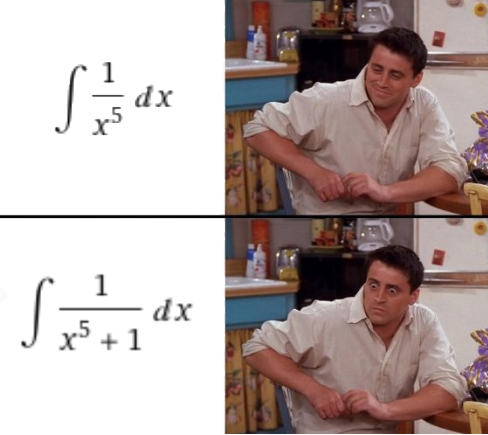
\includegraphics[scale=0.4]{image/integrate_meme.png}
    %\caption{Caption}
\end{figure}
在实分析I这里, 我们终于不(怎么)要计算啦! 掌握了勒贝格积分的定义与基本性质之后, 我们将从``空间"的视角俯瞰勒贝格可积函数构成的集合. 
什么是``空间"? 我不给出精确的定义\footnote{这个名词本身就很笼统}, 
只给出一些具体语境, 相信大家会有自己的理解.
\begin{enumerate}
    \item 称集合$V$为向量\textbf{空间}若$V$上定义了两种运算: 加法与数乘, 且它们满足众所周知的8条性质. 
    \item 称集合$X$为度量\textbf{空间}(metric space)若$X$配备了一个度量$d$. 记作$(X, d)$.
    \item 称集合$X$为赋范\textbf{空间}(normed space)若$X$配备了一个范数$\norm{\cdot}$.
    \item 称集合$X$为拓扑\textbf{空间}(topological space)若$X$配备了一个拓扑$\calT$. 记作$(X, \calT)$.
\end{enumerate}
\begin{exercise}
    再想出一个``空间"的例子.
\end{exercise}

函数列的收敛问题在分析学的历史上也算是一大热点. 
在数学分析中我们遇到过两种收敛性:
\begin{enumerate}
    \item 逐点收敛, 即$f_n(x) \to f(x)$对每个$x$都成立. 对给定的$x$, $\{f_n(x):n \in \N\}$就是个数列, 并没有什么新内容.
    \item 一致收敛, 即$\lim_{n \to \infty}f_n(x)=f(x)$对$x$一致成立, 这个要比逐点收敛复杂得多.
\end{enumerate}
逐点收敛实质上是依$\R$中的绝对值度量收敛: 一列函数$f_n$在每个点的值越来越``接近"$f$在每个对应点的值, 一致收敛实质上是依连续函数空间上的上确界范数收敛, 该范数用以衡量两个连续函数间的``距离".
在研究极限与积分运算交换次序时, 我们隐约感觉到可以用积分来衡量两个函数之间的距离. 单调收敛定理的结论为
$$\int f_n(x)dx \to \int f(x)dx \quad (n \to \infty),$$
移项得
$$\left|\int f_n(x)-f(x) dx \right| \to 0 \quad (n \to \infty).$$
该式的一个充分条件为
$$\int |f_n(x)-f(x)| dx \to 0 \quad (n \to \infty).$$
不知为什么, 这个式子看着要更顺眼一点. 将其作为衡量函数距离的尺子, 我们定义距离函数
$$d(f,g) = \int |f(x)-g(x)|dx. $$
这样
$(L^1(\R^d), d)$便成为一度量空间, 一般直接写为$L^1(\R^d)$, 或$L^1$. 
如果说度量衡量了两个函数的距离, 那么范数衡量的就是一个函数和原点(向量空间中的$0$元)的距离. 度量很自然地引导出范数:
$$\norm{f-g} = d(f, g), \quad \norm{f} = \int |f(x)|dx. $$

为了熟悉一下绝对值之外的度量/范数, 请完成该练习:
\begin{exercise}
    写出$\{f_n:n \in \N\}$依$L^1(\R^d)$的度量为一个Cauchy列的定义. 
\end{exercise}

在正课中我们学习了$L^1$空间的两大重要性质:
\begin{enumerate}
    \item 完备性: 若$\{f_n:n \in \N\}$是$L^1$中的Cauchy列, 则$f_n$在$L^1$中收敛至一个$L^1$函数$f$. 
    \item $L^1$连续性:
    $$\int |f(x+h)-f(x)|dx \to 0 \quad (h \to 0), $$
    用新型记号来写就是\footnote{有的书会定义成$\tau_h(x)=x-h$, 请以实际教材为准.}
    $$\norm{f \circ \tau_h - f}_{L^1} \to 0 \quad (h \to 0),$$
    其中$\tau_h$为平移映射, $\tau_h: \R^d \to \R^d$, $\tau_h(x) = x+h$. \\
    若定义$$F(h)=\int |f(x+h)-f(x)|dx,$$
    则有$F(h) \to 0~(h \to 0)$. 
\end{enumerate}


我们的老朋友, Riemann可积函数构成的度量空间(配备$L^1$度量)
$\calR$就没有这么好的性质. 
下面的反例说明$\calR$不完备.

\begin{example}\footnote{Fourier Analysis: An Introduction, Stein, exercise 3.5}
    令
    $$f(\theta) = \begin{cases}
        0, & \theta = 0 \\
        \log(1/\theta), & 0 < \theta \leq 2\pi,
    \end{cases}$$
    并定义$\calR$中的函数列$\{f_n: n \in \N\}$为
    $$f_n(\theta) = \begin{cases}
        0,         & 0 \leq \theta \leq 1/n \\
        f(\theta), & 1/n < \theta \leq 2\pi.
    \end{cases}$$
    证明$\{f_n: n \in \N\}$是$\calR$中的Cauchy列, 但$f \notin \calR$. 
\end{example}

% \subsection{Fourier变换初见}
% Stein Fourier Analysis Intro Chap 5 motivation
\begin{example}[~(黎曼-勒贝格引理)]
    对$L^1(\R)$中的函数$f$, 其Fourier变换为
    $\hat{f}(\xi) = \intR f(x)\FourierBase{x\xi}dx$.
    证明当$|\xi| \to \infty$时, $\hat{f}(\xi) \to 0$.
\end{example}
\begin{proof}

    由积分的平移不变性, 将$x$平移$\xi'$后不改变积分值. 于是对所有$\xi' \in \R$, 都有 
    $$\hat{f}(\xi) = \intR f(x)e^{-2\pi ix\xi}dx 
    = \intR f(x-\xi')e^{-2\pi i(x-\xi')\xi}dx.$$
    现取$\xi' = \frac{1}{2}\frac{\xi}{|\xi|^2}$, 有
    \begin{align*}
    \hat{f}(\xi) &= \intR f(x-\xi')\FourierBase{(x\xi - 1/2)}dx \\
    &= \intR f(x-\xi')\FourierBase{x\xi}e^{i\pi}dx \\
    &= -\intR f(x-\xi')\FourierBase{x\xi}dx, 
    \end{align*}
    这样我们把$\hat{f}(\xi)$写成了两种形式, 各取其半, 得 
    $$\hat{f}(\xi) = \frac{1}{2} \intR[f(x)-f(x-\xi')]\FourierBase{x\xi}dx.$$
    
    令$|\xi| \to \infty$, 则$\xi' = \frac{\xi}{2|\xi|^2} \to 0$,
    由积分的$L^1$连续性得
    $$|\hat{f}(\xi)| \leq \frac{1}{2}
     \intR|f(x)-f(x-\xi')|dx\to 0 \quad (\xi \to \infty).$$ \qed 
\end{proof}


\section{最有用的Fubini-Tonelli定理}
如果要评选出实变函数中最常用的两个定理, 我会毫不犹豫地选出“控制收敛定理”和“Fubini定理”. 
Fubini定理的核心是将重积分转化成累次积分, 而交换积分次序则是非常自然的推论. 
在应用中, Tonelli定理与Fubini定理常常成对出现. 我们往往要通过交换积分次序来降低计算难度: 按照第一种次序可能根本算不出来, 按照第二种次序可能就很快算出来了. 而只有算出来了我们才知道这个函数可不可积, 所以Tonelli定理保证了我们在不知道函数可积性的情况下也能进行换序! 
\begin{theorem}[Tonelli]
    设$f(x,y)$是定义在$\R^{d_1} \times \R^{d_2}$上的非负可测函数. 对几乎处处的$y \in \R^{d_2}$, 有
    \begin{enumerate}
    \item $f^y$在$\R^{d_1}$上可测, 
    \item 函数$y \mapsto \int_{\R^{d_1}} f^{y}(x)dx$在$\R^{d_2}$上可测,
    \item 重积分可化为累次积分:
    $$\intRd f(x,y)dxdy = \Lint{\R^{d_2}} \Brace{\Lint{\R^{d_1}}f(x,y)dx}dy.$$
    该等号在扩充实数系上也成立, 即: 若右边的累次积分等于$\infty$, 则左边的重积分也等于$\infty$ (也即$f$不可积). 
    \end{enumerate}
\end{theorem}
\begin{theorem}[Fubini]
    设$f(x,y)$在$\R^{d_1} \times \R^{d_2}$上可积. 那么对几乎处处的$y \in \R^{d_2}$, 有:
    \begin{enumerate}
    \item $f^y$在$\R^{d_1}$上可积,
    \item 函数$y \mapsto \int_{\R^{d_1}} f^{y}(x)dx$在$\R^{d_2}$上可积,
    \item 重积分可化为累次积分:
    $$\intRd f(x,y)dxdy = \Lint{\R^{d_2}} \Brace{\Lint{\R^{d_1}}f(x,y)dx}dy.$$
    \end{enumerate}
\end{theorem}
由于$x$和$y$是对等的, 所以我们很自然地推出积分次序可以交换. 如果不嫌麻烦, 不妨把定理再抄一遍:
\begin{theorem}[Fubini定理再抄一遍]
    设$f(x,y)$在$\R^{d_1} \times \R^{d_2}$上可积. 那么对几乎处处的$x \in \R^{d_1}$, 有:
    \begin{enumerate}
    \item $f_x$在$\R^{d_2}$上可积,
    \item 函数$x \mapsto \int_{\R^{d_2}} f_{x}(y)dy$在$\R^{d_1}$上可积,
    \item 重积分可化为累次积分:
    $$\intRd f(x,y)dxdy = \Lint{\R^{d_1}} \Brace{\Lint{\R^{d_2}}f(x,y)dy}dx.$$
    \end{enumerate}
\end{theorem}
这样, 以$\intRd f(x,y) dxdy$作为桥梁, 我们得到等式
$$\Lint{\R^{d_2}} \Brace{\Lint{\R^{d_1}}f(x,y)dx}dy
  =\Lint{\R^{d_1}} \Brace{\Lint{\R^{d_2}}f(x,y)dy}dx.$$
\begin{remark}
    假如要算一个函数$f(x,y)$的积分, 一般先用Tonelli定理计算$|f|$的积分(满足定理条件: 非负可测).
    把重积分转化成累次积分, 选择一个方便计算的积分次序. 
    如果算出来一个有限数, 就说明$f$可积, 再调用Fubini定理累次计算$f$的积分即可.
\end{remark}

\subsection{纯换序的计算}
接下来, 我们继续介绍Fourier变换的知识, 让大家熟悉Fubini定理的应用(顺便复习积分变量的伸缩变换). 首先来看一个无处不在(物理, 概率论, 统计学...)的函数: Gaussian.
\footnote{Gauss的形容词形式, 一般可用于形容某事物具有正态分布的特点, 也可以当作名词, 这里指形如$e^{-a|x|^2}$的函数.}
\begin{example}[~(Gaussian)]
    若$a>0$, 则
    $$I_n := \int_{\R^n}e^{-a|x|^2}dx = \Brace{\frac{\pi}{a}}^{n/2},$$
    其中$x=(x_1, \cdots, x_n) \in \R^n$, $|x|^2 = x_1^2 + \cdots x_d^2$.
\end{example}
\begin{proof}
    我们迭代地套用Tonelli定理:
    \begin{align*}
    \Lint{\R^n}e^{-a|x|^2}dx 
    &= \Lint{\R^n}e^{-a(x_1^2+\cdots+x_n^2)} dx_1 \cdots dx_n \\
    &= \Lint{\R^{n-1}}\Brace{\Lint{\R^1}e^{-a(x_1^2+\cdots+x_n^2)}dx_1 }dx_2 \cdots dx_n \\
    &= \Lint{\R^{n-1}}\Brace{\Lint{\R^1}e^{-ax_2^2-\cdots-ax_n^2}e^{-ax_1^2}dx_1} 
       dx_2 \cdots dx_n \\
    &= \Lint{\R^{n-1}}e^{-ax_2^2-\cdots-ax_n^2} \Brace{\Lint{\R^1}e^{-ax_1^2}dx_1} 
       dx_2 \cdots dx_n \\
    &= \cdots \\
    &= \Brace{\intR e^{-ax_1^2}dx_1} \cdots \Brace{\intR e^{-ax_n^2}dx_n} \\
    &= \Brace{\intR e^{-ax_1^2}dx_1}^n.
    \end{align*}
    所以只需要对$x \in \R$计算$\intR e^{-ax^2}dx$, 而我们在数学分析中见过这种积分, 参考脑海中的记忆, 由极坐标换元得
    \begin{align*}
    \Brace{\intR e^{-ax^2}dx}^2
    &= \Brace{\intR e^{-ax^2}dx}\Brace{\intR e^{-ay^2}dy} \\
    &= \iint e^{-a(x^2+y^2)} dxdy \\
    &= 2\pi \int_0^\infty e^{-ar^2}r dr \\
    &= \frac{\pi}{a}. 
    \end{align*}
    故$I_1=\sqrt{\pi/a}$. 好巧不巧, $e^{-ax^2}$还是非负的, 所以
    $$\Lint{\R^n}e^{-a|x|^2}dx = \left(\frac{\pi}{a}\right)^{n/2},$$
    这就说明$e^{-a|x|^2}$在$\R^n$上可积, 最后再由Fubini定理得$\Lint{\R^n}e^{-a|x|^2}dx = \left(\frac{\pi}{a}\right)^{n/2}$.
    \qed 
\end{proof}
% 再补一个不是非负函数的例子 (还没找好)

\begin{remark}
    大部分情况我们并不需要一板一眼地先用Tonelli定理证明可积, 再由Fubini定理得积分值. 以下的步骤足以涵盖大多数应用场景:
    \begin{enumerate}
    \item 选择合适的积分次序计算$\int |f(x,y)|dxdy$,
    \item 若算出来$\int |f(x,y)|dxdy<\infty$, 则选择合适的积分次序计算$\int f(x,y)dxdy$,
    \item 结束!
    \end{enumerate}
    如果$f$恰好是非负的, 我们只需完成第一步即可.
\end{remark}

\begin{exercise}
    假装我们已经知道$e^{-\pi x^2}$的Fourier变换是其自身:
    $$\intR e^{-\pi x^2}e^{2\pi ix \xi}dx = e^{-\pi \xi^2}, x, \xi \in \R.$$
    现设$x, \xi \in \R^d$, 计算
    \begin{enumerate}
    \item $$\intRd e^{-\pi |x|^2}\FourierBase{x \cdot \xi}dx;$$
    \item $$\intRd e^{-\pi |x|^2 / \d}\FourierBase{x \cdot \xi}dx.$$
    \end{enumerate}
\end{exercise}

在\ref{L1_space}中我们知道一个$L^1$函数的Fourier变换$\hat{f}$连续而且$\lim_{|\xi|\to \infty}\hat{f}(\xi) = 0$, 这就引出一个非常自然的问题: $\hat{f}$也可积吗? 如果$\hat{f}$也可积, 那么Fourier变换就是$L^1(\R^d)$到自身上的映射. 下面的例题否定了这个猜想. 在该例题中, 我们将会综合运用以下知识点:
\begin{itemize}
    \item 积分变量的伸缩性质
    \item Fubini定理
    \item $\Ga$函数的性质\footnote{如果忘了$\Ga$函数, 可参考任一数学分析教材或者本讲义的附录}
    
\end{itemize}
\begin{example}\footnote{Real Analysis, Stein, exercise 2.25}
    {\everymath{\displaystyle}
    证明对每个固定的$\eps > 0$, 关于$\zeta$的函数$F(\xi)=\frac{1}{(1+|\xi|^2)^\eps}$
    是某个$L^1$函数的Fourier变换. \\
    \textbf{提示}: 令$K_\delta(x)=e^{-\pi|x|^2/\delta} \delta^{-d/2}$, 考虑
    $f(x)=\int_0^\infty K_\delta(x)e^{-\pi \delta}\delta^{\eps-1} d\delta$. 
    应用Fubini定理证明$f \in L^1(\R^d)$, 且$$\hat{f}(\xi) = \int_0^\infty e^{-\pi \delta |\xi|^2} e^{-\pi \delta} \delta^{\eps-1} d\delta, $$
    然后计算这个积分(用gamma函数表达), 结果应为
    $\pi^{-\eps}\Gamma(\eps)\frac{1}{(1+|\xi|^2)^\eps}$.
    }
\end{example}
\begin{proof}
    \begin{align*}
    \intRd f(x)dx
    &= \intR \Brace{\intRd e^{-\pi |x|^2/\d}dx}e^{-\pi \d}\d^{-\frac{d}{2}+\eps-1}d\d \\
    &= \intR \Brace{\frac{\d}{\pi}\pi}^{d/2}e^{-\pi \d}\d^{-\frac{d}{2}+\eps-1}d\d \\
    &= \intR e^{-\pi \d}\d^{\eps-1}d\d \\
    &= \pi^{1-\eps}\intR e^{-\pi \d}(\pi\d)^{\eps-1}d\d \\
    &= \pi^{-\eps}\intR e^{-\pi \d}(\pi\d)^{\eps-1}d(\pi\d) \\
    &= \pi^{-\eps}\Ga(\eps) < \infty,
    \end{align*}
    hence $f \in L^1(\R^d)$. Next, 
    \begin{align*}
    \hat{f}(\xi)
    &= \intRd f(x) \FourierBase{x\cdot \xi}dx \\
    &= \intR_d \Brace{\intR e^{-\pi |x|^2/\d} e^{-\pi \d}\d^{-\frac{d}   {2}+\eps-1} d\d} \FourierBase{x\cdot \xi}dx \\
    &= \intR \Brace{\intRd e^{-\pi |x|^2/\d}
       \FourierBase{x\cdot \xi}dx}e^{-\pi \d} % another FT
       \d^{-\frac{d}{2}+\eps-1} d\d \\
    \end{align*}
    Let $g(x)=e^{-\pi|x|^2/\d},$ then $g(\d^{1/2}|x|)=e^{-\pi|x|^2}$, 
    so $g(\d^{1/2}|x|) \longrightarrow \d^{-d/2}\hat{g}(\d^{-1/2}\xi) = e^{-\pi|\xi|^2}$. From this we get $\hat{g}(\xi)=\d^{d/2}e^{-\pi \d|\xi|^2}$. 
    Continue,
    \begin{align*}
    \hat{f}(\xi)
    &= \int_0^\infty e^{-\pi \delta |\xi|^2} e^{-\pi \delta} \delta^{\eps-1} d\delta \\
    &= \intR e^{-\pi(1+|\xi|^2)\d}\d^{\eps-1}d\d \\
    &= \intR e^{-\pi(1+|\xi|^2)\d}(\pi(1+|\xi|^2)\d)^{\eps-1}
       (\pi(1+|\xi|^2))^{1-\eps} d\d \\
    &= \pi^{-\eps}(1+|\xi|^2)^{-\eps} 
       \intR e^{\pi(1+|\xi|^2)\d}(\pi(1+|\xi|^2)\d)^{\eps-1} 
       d(\pi(1+|\xi|^2)\d) \\
    &= \pi^{-\eps}\Ga(\eps)\frac{1}{(1+|\xi|^2)^\eps}
    \end{align*}
    Once $\eps$ is given, $\Ga(\eps)$ is a constant. 
    We have shown that $\pi^{-\eps}\Ga(\eps)\frac{1}{(1+|\xi|^2)^\eps}$ is the Fourier transform of $f$. \qed
\end{proof}
\begin{remark}
    If we take $\eps=1/2$ and let $d=1$ 
    then calculus tells us 
    $$ \int \frac{1}{\sqrt{1+\xi^2}}d\xi 
       = \log (\xi + \sqrt{\xi^2 + 1}) + C, $$
    hence $\intR \frac{1}{\sqrt{1+\xi^2}}d\xi$ diverges. 
\end{remark}

\subsection{积分区域的切片}
不知大家有没有发现, 刚才几个例子的积分区域\footnote{这里的区域泛指做积分的可测集, 而非有界开集}
都是$\R$或者更一般的$\R^n$, 所以我们在换序时不需要考虑积分区域的变化. 回忆一下我们在微积分/数学分析中是怎么计算二重积分的: 将积分区域写成所谓的``$x$型区域"或``$y$型区域", 再进行累次积分. 
而在Fubini定理中, 积分区域看似都是$\R^d, \R^{d_1}, \R^{d_2}$, 实则吸收于被积函数$f$中: $$\int_E f(x,y) dxdy = \intRd f(x, y) \chi_E (x,y) dxdy. $$
做累次积分就会出现
$$\int_{\R^{d_1}} f(x,y) \chi_E (x,y) dx, $$
此时被积函数就可看作$y$固定, $x$在动的切片$(f \chi_E)^y(x) = f^y(x) (\chi_E)^y(x)$. 考虑$d_1=d_2=1$的二重积分情形, $(\chi_E)^y(x)$ 与积分号 $
\intR$ 碰一碰就能产生
$$\intR f^y(x) (\chi_E)^y(x) dx = \int_{E^y} f^y(x) dx!$$
这就是我们在微积分中做的事: 找切片区域. 我们马上看一个具体的例子:
\begin{example}[~(分布函数)]
    设$f$是$\R^d$上的可测函数, 定义$f$的\textit{分布函数}$d_f: [0, \infty) \to [0, \infty]$为 
    $$d_f(\a) = m(\{x \in \R^d: |f(x)| > \a\}).$$ 
    设
    $|f|^p \in L^1, 0<p<\infty$.
    证明
    $$\|f\|_{L^p}^p := \intRd |f|^p d\mu = p \int_0^\infty \a^{p-1}d_f(\a) d\a. $$
\end{example}
\begin{proof}
    将分布函数中的测度还原成积分形式, 得
    \begin{align*}
    p \int_0^\infty \a^{p-1}d_f(\a) d\a
    &= p \int_0^\infty \a^{p-1} \int_X \chi_{\{x:|f(x)|>\a\}} dm(x) 
        d\a. 
    \end{align*}
    开始换序! 我们需要给特征函数做切片, 严格复制粘贴定义得
    $$\chi_{\{x:|f(x)|>\a\}}(x, \a) = 
    \begin{cases}
        0 & \text{若 } |f(x)| \leq \a, \\
        1 & \text{若 } |f(x)| > \a.
    \end{cases}$$
    固定住$x$, 则$\chi$的$x$-切片为
    $$\chi_{\{x:|f(x)|>\a \}}(\a) = 
    \begin{cases}
        0 & \text{若 } \a \geq |f(x)|, \\
        1 & \text{若 } \a < |f(x)|.
    \end{cases}$$
    所以, 
    \begin{align*}
    p\int_0^\infty \a^{p-1} \intRd \chi_{\{x:|f(x)|>\a\}} dm(x)d\a
    &= p\intRd \int_0^\infty \a^{p-1} \chi_{\{x:\a < |f(x)| \}}(\a) d\a dm(x) \\
    &= \intRd \int_0^{|f(x)|} pa^{p-1} d\a dm(x) \\
    &= \intRd |f(x)|^p dm(x).
    \end{align*}
    \qed
\end{proof}
\begin{remark}
    在微积分中, 积分区域一般都是矩形, 三角形等肉眼可以看出切片的集合, 但在实分析中我们遇到的大多是抽象的集合, 正如上例. 强烈建议初学者严格按照``特征函数 $+$ 在整个空间上积分"的形式进行计算. 
\end{remark}
\begin{exercise}
    设$f \in L^1(\R)$, 令$F(x) = \int_{-\infty}^x f(t)~dt$, 证明$F$连续.
\end{exercise}
    \section{Littlewood三原则}
英国数学家Littlewood在其著作\textit{Lectures on the Theory of Functions}中作出过如下总结:
\begin{itemize}
    \item 每个可测集``几乎"都是有限多个区间的和;
    \item 每个函数``几乎"都是连续的;
    \item 每个收敛的函数列都``几乎"一致收敛.
\end{itemize}
\begin{figure}[h]
    \centering
    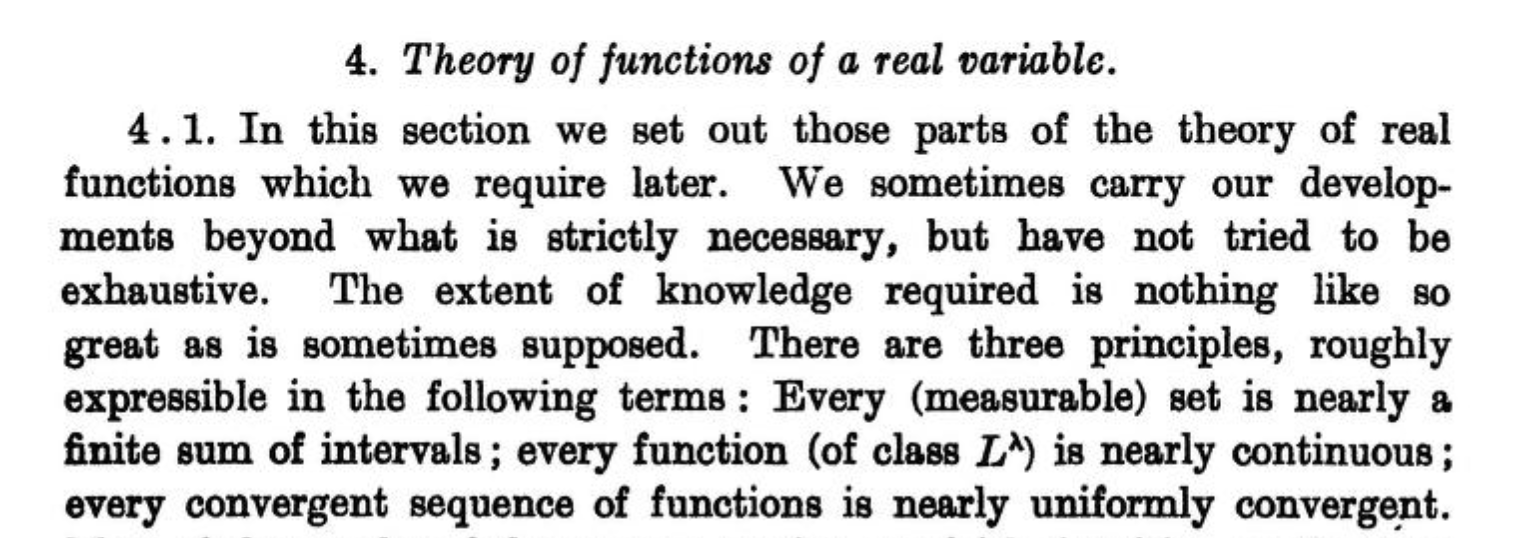
\includegraphics[scale=0.5]{image/Littlewood_3_principles.png}
    \caption{Littlewood, J. E. (1944). \textit{Lectures on the Theory of Functions}.}
    \label{fig:my_label}
\end{figure}
第一条见Lebesgue测度的正规性质, 第三条则是Egorov定理, 第二条是Lusin定理, 可借助Egorov定理推出. 我们首先复习Egorov定理的描述, 再证明Lusin定理. 
\begin{theorem}[Egorov定理]
    设$X \subset \R^d$, $m(X)<\infty$. 设定义在$X$上的可测函数列$f_n$几乎处处收敛于$f$, 则对任意$\eps>0$都存在集合$E, m(X\setminus E)< \eps$且$f_n$在$E$中一致收敛于$f$. 
\end{theorem}

Lusin定理的证明值得细细品味. 虽说这是一个关于可测函数的结论, 但证明借助了积分理论中的工具. 

    \section{难点: 函数列的收敛模式}
% 主要参考Folland 2.4
论证极限与积分次序可以交换的最常用的工具是单调收敛定理与控制收敛定理. 在控制收敛定理中, 我们其实得到的是更广泛的结论: $\int |f_n - f| \to 0$, 即$\|f_n - f\|_{L^1} \to 0$, 根据三角不等式可得$\int f_n \to \int f$. 当然, 交换次序的充分条件肯定不止上面这两个定理, 其余用途没那么广泛的结论便散落在各个教材的习题, 各个学校的考试中, 悄无声息地消磨萌新学习实变函数的热情. 大家不必感到恐惧, 这部分内容在后续课程中用得很少, 建议仅在考前学习本节. 
\subsection{依测度收敛}
\begin{definition}
    设$\{f_n\}$为一列可测函数. 如果对任意$\eps > 0$, 有
    $$m(\{x: |f_n(x) - f(x)| \geq \eps\}) \to 0 \quad (n \to \infty),$$
    则称$f_n$依测度收敛于$f$. 为下文描述方便, 将其记作$f_n \xrightarrow[]{m} f$. 
\end{definition}
首先, 这是我们非常熟悉的数列收敛. 对每个$n$, 把$f_n(x)$离$f(x)$不是那么近的点挑出来, 量出它的测度, 得到一个数列. 依测度收敛说得便是这个数列趋于0:
那些离$f(x)$有些远的点``越来越少".
\begin{exercise}
    写出依测度收敛的否定.
\end{exercise}
\begin{exercise}
    证明: 若$f_n \xrightarrow[]{m} f$, 则$\{f_n\}$的任一子列也依测度收敛于$f$. 
\end{exercise}
\begin{exercise}
    判断: 对可测函数列$\{f_n\}$, 若对任意$\eps>0$, 有
    $$m(\{x: |f_n(x) - f(x)| > \eps\}) \to 0 \quad (n \to \infty),$$
    那么$f_n$依测度收敛于$f$吗?
\end{exercise}
\begin{exercise}
    $f_n$依测度收敛于$f$当且仅当
    $$\forall \eps > 0 ~\exists N \in \N: 
    \mu(\{x:|f_n(x)-f(x)| \geq \eps\}) < \eps ~\forall n \geq N.$$
\end{exercise}
我们列出两个常用结论:
% 看maki正课讲不讲
\begin{proposition}
    \begin{enumerate}
    \item 如果$\|f_n - f\|_{L^1} \to 0$, 则$f_n$依测度收敛于$f$. 
    \item 如果$f_n$依测度收敛于$f$, 则存在子列$\{f_{n_j}\}$几乎处处收敛于$f$. 注意, 此处并非一致收敛, 而是对几乎处处的$x$, 有$f_{n_j}(x) \to f(x)~(j \to \infty)$.
\end{enumerate}
\end{proposition}
依测度收敛也可由度量导出.
\begin{example}
    设$X \subset \R^d, m(X)<\infty$, $f, g: X \to \R$. 定义
    $$\rho(f,g) = \int \frac{|f(x)-g(x)|}{1+|f(x)-g(x)|}dx.$$
    证明
    \begin{enumerate}
        \item $\rho$是可测函数构成的向量空间上的度量.
        \item $\rho(f_n, f) \to 0$当且仅当$f_n$依测度收敛于$f$. 
    \end{enumerate}
\end{example}
\begin{proof}
    第一问留作习题: 证明三角不等式可以考虑利用函数$1/(1+x)$的性质.
    设$f_n \xrightarrow[]{m} f$, 设$\eps > 0$, 则
    $$m(\{x:|f_n(x)-f(x)| \geq \eps\}) \to 0 \quad n \to \infty.$$
    我们发现$m$里面的集合非常有用, 记$A_{n, \eps} = \{x:|f_n(x)-f(x)| \geq \eps\},$ 则$A_{n, \eps}^c = \{x:|f_n(x)-f(x)| < \eps\}$. 于是,
    \begin{align*}
    \int \frac{|f_n(x)-f(x)|}{1+|f_n(x)-f(x)|}dx
    &= \int_{A_{n,\eps}}\frac{|f_n(x)-f(x)|}{1+|f_n(x)-f(x)|}dx 
       + \int_{A_{n,\eps}^c}\frac{|f_n(x)-f(x)|}{1+|f_n(x)-f(x)|}dx \\
    &\leq m(A_{n, \eps}) + \eps m(X).
    \end{align*}
    由依测度收敛的定义, 当$n$非常大时, 有
    $m(\{x:|f_n(x)-f(x)| \geq \eps\}) < \eps$ (这两个$\eps$并不矛盾!), 则$$ m(A_{n,\eps}) + \eps m(X) < (1+m(X))\eps, $$ 
    所以$\rho(f_n, f) \to 0$. 

    反过来, 设$\rho(f_n, f) \to 0$. 记$g_n(x) =  \frac{|f_n(x)-f(x)|}{1+|f_n(x)-f(x)|}$, 设$\eps > 0$, 记
    $G_{n,\eps} = \{x: g_n(x) \geq \eps\}$. 则
    $$\int g_n(x)dx = \int_{G_{n,\eps}}g_n(x)dx + 
      \int_{G_{n,\eps}^c} g_n(x)dx \geq \eps m(G_{n,\eps})
      +  \int_{G_{n,\eps}^c} g_n(x)dx, $$
    令$n \to \infty$, 则$\eps \mu(G_{n,\eps}) \to 0$. 由于$\eps$取定, 故$ \mu(G_{n,\eps}) \to 0 $.
    最后, 
    $$\frac{|f_n(x)-f(x)|}{1+|f_n(x)-f(x)|}>\eps \implies 
    |f_n(x)-f(x)| > \frac{\eps}{1-\eps}.$$
    当$\eps$取遍所有正数时, $\eps/(1-\eps)$也能取遍所有正数, 因为
    $\eps \mapsto \eps/(1-\eps)$为满射. 我们得到结论: $f_n \xrightarrow[]{m} f$.
\end{proof}
\begin{remark}
    我们挖掘一些上述证明过程中的注意点\footnote{在此感谢2022年秋学期在UW-Madison上Math 721的同学, 你们作业中的问题提供了足量的素材, 让我总结出了一些注意事项. }. 
    \begin{enumerate}
    \item 养成良好的习惯: 给集合$\{x:|f_n(x)-f(x)| \geq \eps\}$取名字时最好不要直接给个字母$A$, 因为$n$在变, $\eps$在有需要时也会变, 取记号时应该包含这些信息, 用上下标或括号的形式体现出来, 如
    $$A_{n,\eps},\quad A_n^\eps,\quad A(n,\eps), \quad \cdots$$
    \item 证明的核心步骤利用了一种``微妙的平衡": 函数值大的集合测度小, 函数值小的集合测度是有限的. 之后我们会常常用到这一思想.
    \end{enumerate}
\end{remark}
\begin{example}
    设$f_n$依测度收敛于$f$, $g_n$依测度收敛于$g$. 则
    \begin{enumerate}
    \item $f_n+g_n$依测度收敛于$f+g$.
    \item 若$f_n, g_n$定义在有限测度集上, 则$f_ng_n$依测度收敛于$fg$. 
    \end{enumerate}
\end{example}

\begin{exercise}
    若$f_n \geq 0$且$f_n$依测度收敛于$f$, 则$\int f \leq \liminf_{n \to \infty}\int f_n$.
\end{exercise}




\subsection{还有哪些条件可以保证换序?}
控制收敛定理因其条件简单而获得广泛应用. 保留住``$f_n \to f$ a.e."这一条件, 还有哪些假设能够保证$\int f_n \to \int f$? 我们以Vitali收敛定理作为例子. 

\begin{definition}[一致可积]
    设$\{f_n\}_{n \in \N}$为一列定义在集合$E$上的可测函数, 其中$m(E) < \infty$. 如果对任意的$\eps>0$都存在$\d>0$, 当$m(E)<\delta$时, 有
    $$\sup_{n \in \N} \abs{\int_E f_n(x) dx} < \eps,$$
    则称$\{f_n\}_{n \in \N}$一致可积(uniformly integrable).
\end{definition}
此时大家肯定想到了积分的绝对连续性: 只要集合够小, 可积函数在这个集合上的积分就可以足够小. 一致可积性不过是把单个函数的绝对连续性推广至了一列函数的绝对连续性. 
\begin{example}[~(Vitali收敛定理·简单版本)]
    设$X \subset \R^d, m(X) < \infty$, $\{f_n\}_{n \in \N}$一致可积, 且$f_n(x) \to f(x)$ a.e., $|f(x)|$几乎处处有限. 证明
    $$\lim_{n \to \infty} \int_E f_n(x)dx = \int_E f(x)dx.$$
\end{example}
\begin{proof}
    令$\eps>0$, 则由一致可积性知存在$\d>0$, 可测集$A$只要满足$m(A) < \d$就能推出$\int_A |f_n(x)|dx < \eps~\forall n \in \N$. $f_n$几乎处处收敛于$f$的最大问题是缺乏一致性, 所以不能直接放到积分号下进行估计. 应用Egorov定理\footnote{不要忘了Egorov定理的条件: 函数列定义在有限测度集上. 这里$m(X)<\infty$满足定理的假设.}
    可以让$\{f_n\}_{n \in \N}$在一个``很小"的集合外一致收敛. 对刚才取好的$\d$, 存在集合$E: m(E) < \d$且$f_n$在$E^c$中一致收敛于$f$. 于是,
    \begin{align*}
        \int_X |f_n(x)-f(x)|dx
        &= \int_E |f_n(x)-f(x)|dx + \int_{E^c}|f_n(x)-f(x)|dx \\
        &\leq \int_E |f_n(x)|dx + \int_E |f(x)|dx + \int_{E^c}|f_n(x)-f(x)|dx.
    \end{align*}
    由一致可积性知$\int_E |f_n(x)|dx < \eps$, 由一致收敛性知$\int_{E^c}|f_n(x)-f(x)|dx < \eps$(当$n$非常大时), 现在只剩下中间一项. 数列极限有个非常有用的性质: 保不等式性. 一个收敛数列如果每项都小于等于$M$, 那么它的极限也不会超过$M$. 但是这里我们并没有$f_n$一致收敛于$f$, 所以无法跨过积分这道坎, 这时就该请出Fatou引理了:
    \begin{align*}
        \int_E |f(x)|dx
        &= \int_E \liminf_{n \to \infty} |f_n(x)|dx \quad 
           (f_n(x) \to f(x) \text{ a.e.})\\
        &\leq \liminf_{n \to \infty} \int_E |f_n(x)|dx \quad 
              (\text{Fatou引理})\\
        &< \eps. \quad (\text{一致可积性, } m(E) < \delta)
    \end{align*}
    三剑合璧, 得
    $$\int_X |f_n(x)-f(x)|dx < 3\eps,$$
    定理得证. \qed
\end{proof}
接下来的练习主要研究哪些假设能够保证极限与积分交换次序. 这些题目的结论都是$\lim_{n \to \infty}\int f_n = \int f$或$\lim_{n \to \infty}\int |f_n-f|=0$. 根据三角不等式, 后者可以推出前者.
\begin{exercise}
    利用Vitali收敛定理推出控制收敛定理.
\end{exercise}
\begin{proof}
    提示: 将$\R^d$拆成$E \cup E^c$, 其中$E$为有限测度集, 且控制函数$g$的积分都``集中"在$E$上. 
\end{proof}
\begin{exercise}
    设$f_n: X \to \R, m(X) < \infty$ 且 $\{f_n\}_{n \in \N} \subset L^1$, $f_n$一致收敛于$f$. 证明$f \in L^1$且$\int f_n \to \int f$.  
\end{exercise}
\begin{exercise} % Folland ex 2.20
    (推广的控制收敛定理) 令$f_n, g_n, f, g \in L^1, f_n \to f$ a.e., $g_n \to g$ a.e., $|f_n| \leq g_n, \int g_n \to \int g$, 则
    $\int f_n \to \int f$. 
\end{exercise}

\begin{exercise}
    设$f_n \geq 0$, $f_n$依测度收敛于$f$, 则$\int f \leq \liminf_{n \to \infty} \int f_n$.
\end{exercise}
\begin{proof}
    提示: 数列的下极限就是其某个子列的极限; 由$f_n$依测度收敛于$f$可知$\{f_n\}$有一个几乎处处(逐点)收敛的子列.
\end{proof}
\begin{exercise}
    设$|f_n|\leq g \in L^1, f_n$依测度收敛于$f$. 证明
    \begin{enumerate}
        \item $\int f = \lim \int f_n$.
        \item $\|f_n - f\|_{L^1} \to 0$.
    \end{enumerate}
\end{exercise}
\begin{exercise}
    设$f_n, f \in L^1, f_n \to f$ a.e. 则$\int |f_n-f| \to 0$当且仅当
    $\int |f_n| \to \int |f|$. 
\end{exercise}
\begin{exercise} % Math 721 HW 3 Fall 2022
    
\end{exercise}


\subsection{收敛性大杂烩}
函数列的各种收敛性绝对是萌新学习实变函数的一大噩梦, 不过这部分内容后面用得很少, 如果不是为了准备考试, 第一遍学时完全可以跳过. 目前为止, 我们学习过以下(包括但不限于)收敛性:
\begin{itemize}
    \item 一致收敛;
    \item 几乎处处收敛;
    \item $L^1$收敛: $\int |f_n-f| \to 0$;
    \item 换序收敛: $\int f_n \to \int f$;
    \item 依测度收敛.
\end{itemize}
我们先用几个例子说明前3种收敛性的关系. 例子来自Folland, \textit{Real Analysis}的2.4节, 作者本人也建议牢记这些例子.
\begin{enumerate}
    \item $f_n = n^{-1}\chi_{(0,n)}$.
    \item $f_n = \chi_{(n,n+1)}$.
    \item $f_n = n\chi_{[0, 1/n]}$.
    \item (打字机函数列) $f_1=\chi_{[0,1]}, f_2=\chi_{[0,1/2]}, 
    f_3=\chi_{[1/2,1]}, f_4=\chi_{[0,1/4]}, f_5=\chi_{[1/4,1/2]}, 
    f_6=\chi_{[1/2,3/4]}, f_7=\chi_{[3/4,1]}, \cdots. $
\end{enumerate}

\subsection{思想方法总结}





    \section{利用积分理论解决测度问题}
``实分析"是个庞大的体系, 分析学中的各种理论与技巧都可以塞进这个框, 所以Maki's Lab实分析小组将其拆分为三大部分, 以便初学者入门现代分析学. 
实分析I的副标题为``测度与积分", 目前大家可能觉得测度就是测度, 积分就是积分, 但它们可以由特征函数自然地联系起来:
$$m(E) = \int_{\R^d} \chi_{E}(x) dx.$$
学到抽象测度时, 我们会知道: 积分只是测度的一个例子. 

许多问题的题干中只有Lebesgue测度, 看起来像是只用测度的一堆性质就能做出来. 实际上, 这些题需要利用特征函数联系测度与积分, 再利用积分的性质解决. 
\begin{example} %UW-Madison Qual
    设$E \subset \R$可测且具有有限测度. 定义函数$f:\R \to \R$,
    $f(x)=m(E \cap(E+x))$. 证明$f$连续.
\end{example}
\begin{proof}
    
\end{proof}

\begin{example} %UW-Madison Qual
    Let $E \subset[0,1]$ be a Lebesgue measurable set with $m(E)>0.999$. Prove that there exists $\epsilon_0>0$ such that for every $t \in\left(0, \epsilon_0\right)$, we can always find $x$ such that $x, x+t, x+t^2 \in E$.

    Hint: Try estimating $\int_0^1\left(\chi_E(x)+\chi_E(x+t)+\chi_E\left(x+t^2\right)\right) d x$, where $\chi_E$ is the characteristic function of $E$.
\end{example}

\begin{example} %UW-Madison Qual
    Let $E \subset[0,1]$ be a measurable set with positive Lebesgue measure. Let $\chi$ be the characteristic function of $E$.
    (a) Let $F(x)=\int_{\mathbb{R}} \chi(x-t) \chi(t) d t$. Prove that $F$ is a continuous function.
    (b) Let $E+E=\left\{e_1+e_2 \in \mathbb{R} \mid e_1 \in E, e_2 \in E\right\}$. Prove that $E+E$ contains a non-empty open subset of $\mathbb{R}$.
\end{example}


\chapter{函数的微分}
    \section{有界变差函数的判别}

\subsection{直接使用定义判断}

\subsection{利用单调区间进行划分}
直觉上看, 有界变差函数不能
\begin{enumerate}
    \item 振荡得太狠(振幅大);
    \item 振荡得太频繁.
\end{enumerate}
而三角函数是最天然的振荡函数, 只要将$\sin x$中的$x$换一换就能调整频率, 而在$\sin x$前乘上一些函数则能控制振幅. 接下来是一系列关于三角函数的例子.
\begin{example}
    设
    $$f(x)=\begin{cases}
        \sin (1/x), & 0 < x \leq 1 \\
        0,          & x = 0,
    \end{cases}$$
    $f$是有界变差函数吗? 
\end{example}
\begin{solution}
    有界变差函数不能振荡得太频繁, 而当$x$距离$0$越来越近时, $1/x$会增加得越来越快, 从而包含的三角函数的周期区间就越来越多, 也即振荡得越来越频繁, 而且振幅恒为$1$! 有了这个直觉之后, 我们的目标就证明$f$不是有界变差函数. \\
    % 此处插入函数图像
    \begin{center}
    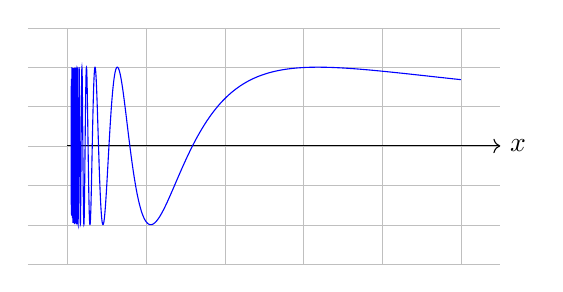
\begin{tikzpicture}[x=5cm]
    \draw[xstep=.2,ystep=.5,lightgray,ultra thin] (-0.1,-1.5) grid (1.1,1.5);
    \draw[->] (0,0) -- (1.1,0) node[right] {$x$};
    %\draw[->] (0,-1) -- (0,1.1) node[above] {$\sin (1/x)$};
    \draw[blue,domain=0.01:1,samples=5000] plot (\x, {sin((1/\x)r)});
    \end{tikzpicture}
    \end{center}
    虽然$\sin(1/x)$整体上振荡得图像都看不见了, 但是在局部上它与普通的三角函数$\sin x$没有本质区别: 在某个区间(即使非常短)内都要从$-1$单调增到$1$, 再单调减到$-1$. 
    记$y=1/x$, 则$\sin y$在$[2k\pi - \pi/2, 2k\pi + \pi/2]$上单调增, 在$[2k\pi + \pi/2, 2k\pi + 3\pi/2]$上单调减. 解不等式
    $$2k\pi - \frac{\pi}{2} \leq \frac{1}{x} \leq 2k\pi + \frac{\pi}{2}, \quad
      2k\pi + \frac{\pi}{2} \leq \frac{1}{x} \leq 2k\pi + \frac{3\pi}{2} $$
    得$\sin(1/x)$在$\displaystyle{\left[\frac{1}{2k\pi+\pi/2}, \frac{1}{2k\pi-\pi/2} \right] := [a_k, b_k]}$上单调增, 
    在$\displaystyle{\left[\frac{1}{2k\pi+3\pi/2}, \frac{1}{2k\pi+\pi/2} \right]} := [c_k, d_k]$上单调减.
    从右往左取分割点:
    $$1, b_1, a_1, d_1, c_1; b_2, a_2, d_2, c_2; \cdots $$
    但是有界变差函数定义中的分割只能有有限多个分割点, 所以我们取一列分割:
    \begin{align*}
        &\calP_1: 1, b_1, a_1, d_1, c_1; 0. \\
        &\calP_2: 1, b_1, a_1, d_1, c_1; b_2, a_2, d_2, c_2; 0. \\
        &\cdots \cdots \\
        &\calP_N: 1, b_1, a_1, d_1, c_1; \cdots; b_N, a_N, d_N, c_N; 0.
    \end{align*}
    在$[c_N, 0]$这一段显然有$|f(c_N)-f(0)| \leq 2\sup_{x\in [0,c_N]}|f(x)| \leq 2$. 在每个单调区间上, 有$|f(b_N)-f(a_N)|=|f(d_N)-f(c_N)|=2$, 所以$T_{\calP_N}(f) \geq 4N$. 也就是说, 对每个正整数$N$我们都能找到划分$\calP_N$使$f$在该划分下的全变差$\geq 4N$, 这就证明了$f$不是有界变差函数. 
\end{solution}                   
现在我们控制一下振幅:
\begin{example}
    设
    $$f(x)=\begin{cases}
        x^2 \sin (1/x), & 0 < x \leq 1 \\
        0,          & x = 0,
    \end{cases}$$
    $f$是有界变差函数吗?
\end{example}



%\begin{solution} % 此处解答错误, 后续更改
%    本例与上例唯一的不同之处在于单个单调区间上的估计:
%    $$|f(b_k)-f(a_k)| \leq \left|\frac{2}{(2k\pi - \pi/2)^2} \right|=O\Brace{\frac{1}{k^2}},$$ 类似地 $|f(d_k)-f(c_k)| \leq O\Brace{1/k^2}$. 最右端同样有$|f(1)-f(b_1)| \leq 2$,
%    所以$$T_{\calP_N}(f) \leq C\Sum{k=1}{N}\frac{1}{k^2}+4 \leq C\frac{\pi^2}{6}+4. $$
%    为何只需说明在\textbf{单调划分}下的变差有界就够了? 我们知道增加分割点会使变差增加(或不变), 现取定一个单调划分$\calP_N$, 往里添加一个分割点$t$:
%    \begin{enumerate}
%        \item 若$t \in (c_N, b_1)$, 则$t$必落在某个单调区间$[a_k,b_k]$(或$[c_k,d_k]$)内, 那么这一区间上的变差就要修正为
%        $$|f(b_k)-f(t)|+|f(t)-f(a_k)|=f(b_k)-f(t)+f(t)-f(a_k)=f(b_k)-f(a_k), $$
%        这与$\calP_N$对应的变差完全一样! 所以这个分割点加了和没加一样.
%        \item 若$t \in (b_1, 1)$, 理由同上(根据图像, $f$在$(b_1,1)$单调减). 
%        \item 如果$t \in (0, c_N)$, 我们要加入更多的单调区间把$t$盖进去. $t>0$意味着$t>\delta>0$, 而
%        $\displaystyle{c_k = \frac{1}{2k\pi + 3\pi/2} \to 0}$意味着存在$\Tilde{N}$使$c_{\Tilde{N}}<\delta<t$, 这样我们又回到了第一种情形, 且有
%        $$T_{\calP_N \cup \{t\}}(f) \leq T_{\calP_{\Tilde{N}}}(f) \leq C\frac{\pi^2}{6}+4.$$
%    \end{enumerate}
%\end{solution}



\begin{exercise} % Stein ex 3-11
    设$a,b>0$, 令
    $$f(x)=\begin{cases}
        x^a \sin (x^{-b}), & 0 < x \leq 1 \\
        0,          & x = 0,
    \end{cases}$$
    找出$f$是有界变差函数的充要条件.
    {[\textbf{提示}: 讨论$\displaystyle{\sum \frac{1}{k^{a/b}}}$的收敛性]}
\end{exercise}
    \input{3 differentiation/2 abs_cts_functions.tex}

\chapter{抽象测度与积分}
    \section{集合-代数结构}


\section{抽象测度的构造}


    \section{积分}

\section{乘积测度}
利用集合-代数结构证明集合的性质.
\begin{example}
    若 $E \in \calM \otimes \calN$, 则$\forall x \in X, E_x \in \calN$ 且 $\forall y \in Y, E^y \in \calM$.
\end{example}
\begin{proof}
    写出定义$E_x=\{y \in Y: (x,y) \in E\}$似乎并没有什么帮助, 我们还是看不出来$E_x$到底长什么样. 这时就要用集合-代数结构避开``$E_x$的模样"这一难题. 我们将要证明的性质``$\forall x \in X, E_x \in \calN$ 且 $\forall y \in Y, E^y \in \calM$"用作集族的描述: 令
    $$\calR = \left\{E \in \calM \otimes \calN: \forall x \in X, E_x \in \calN \text{~且~} \forall y \in Y, E^y \in \calM \right\},$$
    然后研究$\calR$具有什么样的集合-代数结构.
    设$\{E_n:n \in \N\} \in \calR$, 则$\Brace{\bigunion{n=1}{\infty}E_n}_x = \bigunion{n=1}{\infty}(E_n)_x \in \calN$ (因为$\calN$是个$\sigma$-代数). 若$E \in \calR$, 则$(E^c)_x = (E_x)^c \in \calN$. 类似地, $\Brace{\bigunion{n=1}{\infty}E_n}^y \in \calM$ 且
    $(E^c)^y \in \calM$, 这就证明了$\calR$是一个$\sigma$-代数. 
    最后, $\calR$本身包含了所有形如$A \times B (A \in \calM, B \in \calN)$的集合, 而根据定义, 
    $\calM \otimes \calN$又由$\{A \times B: A \in \calM, B \in \calN\}$生成, 所以得包含关系
    $$\calR \supset \calM \otimes \calN.$$ 
    若$E \in \calM \otimes \calN$, 则$E \in \calR$, 则$\forall x \in X, E_x \in \calN$ 且 $\forall y \in Y, E^y \in \calM$.    
\end{proof}

\subsection{Fubini定理}
Fubini定理的条件``$\sigma$-有限"不能少.
\begin{example} % Folland 2.46
    设$X=Y=[0,1], \calM = \calN = \calB_{[0,1]}$, $\mu=$Lebesgue测度, $\nu=$计数测度. 令
    $D=\{(x,x): x\in [0,1]\}$, 则
    $$\iint \chi_D d\mu d\nu, \quad \iint \chi_D d\nu d\mu, \quad \int \chi_D d(\mu \times \nu)$$
    互不相等.
\end{example}

%\chapter{Baire纲定理及泛函分析三大定理}


\end{document}
